\documentclass[UTF8,a4paper,11pt,titlepage,oneside]{ctexbook}

\usepackage[english]{babel}
\usepackage{soul}
% \usepackage{color} % If you want to define colors for code syntax highlighting
\usepackage[x11names]{xcolor} % 使用 x11names 以支持更多颜色
% \usepackage{xcolor}
\usepackage{amssymb}
\usepackage{graphicx}
\usepackage{tabularx}
\usepackage{makecell}
\usepackage{caption}
\usepackage{listings}
\captionsetup[table]{name=表} % 将表的标题设置为“表”
\captionsetup[figure]{name=图} % 将表的标题设置为“表”
\renewcommand{\lstlistingname}{列表} % 将 listing 改为 列表
\usepackage{amsmath}
\usepackage{float}
\usepackage{pifont}
\usepackage{amsfonts}
\usepackage{algorithm}
\usepackage{algorithmic}
\usepackage{bm}
\usepackage{amsmath}
\usepackage{booktabs}
\usepackage{multirow}
\usepackage{url}

\usepackage{lmodern}
\usepackage{makecell}
\usepackage{subcaption}
% \usepackage{subfig}
%\usepackage{subfigure}

\usepackage{comment}
\usepackage{geometry}
\geometry{a4paper,left=3.5cm,right=3.5cm,top=4cm,bottom=5cm}
\usepackage{marvosym}

\usepackage{hyperref}
\definecolor{ForestGreen}{RGB}{0,100,0}
\hypersetup{
    colorlinks=true,
    hypertexnames=false, % 目录、封面与正文页码重置时仍保持链接锚点唯一
    linkcolor=black, % 目录、插图目录、表格目录及内部交叉引用统一黑色
    citecolor=black, % 正文文献引用使用黑色数字标号
    urlcolor=blue
}

% \usepackage[colorlinks=true, linkcolor=red, citecolor=ForestGreen, urlcolor=blue]{hyperref}
% \setlength{\parindent}{2em}

\lstset{
    basicstyle=\ttfamily,
    columns=fullflexible,
    keywordstyle=\color{blue},
    commentstyle=\color{green!40!black},
    stringstyle=\color{red},
}

% \usepackage{subfig}
\usepackage{threeparttable}
\usepackage{tocloft}

% 规定图片路径
\graphicspath{{pic/}}

% 普通页与章节首页统一为页脚居中页码，不使用书籍默认页眉。
\pagestyle{plain}

% 经典数字编号参考文献：正文平排 [1]，列表五号宋体、罗马西文字体，
% 编号左置、正文悬挂对齐；保留标准 BibTeX plain 条目格式。
\makeatletter
\def\@cite#1#2{[{#1\if@tempswa , #2\fi}]}
\renewcommand{\@biblabel}[1]{[#1]}
\renewenvironment{thebibliography}[1]
  {\chapter*{\bibname}%
   \addcontentsline{toc}{chapter}{\bibname}%
   \normalfont\rmfamily\songti\zihao{5}%
   \setlength{\baselineskip}{16pt}%
   \color{black}\hypersetup{urlcolor=black}%
   \list{\@biblabel{\@arabic\c@enumiv}}%
     {\settowidth\labelwidth{\@biblabel{#1}}%
      \setlength{\labelsep}{0.6em}%
      \setlength{\leftmargin}{\labelwidth}%
      \addtolength{\leftmargin}{\labelsep}%
      \setlength{\itemsep}{3pt}%
      \setlength{\parsep}{0pt}%
      \setlength{\topsep}{0pt}%
      \usecounter{enumiv}%
      \let\p@enumiv\@empty
      \renewcommand{\theenumiv}{\@arabic\c@enumiv}}%
   \sloppy\clubpenalty4000\widowpenalty4000\sfcode`\.=1000\relax}
  {\def\@noitemerr{\@latex@warning{Empty `thebibliography' environment}}%
   \endlist}
\makeatother

\begin{document}
\renewcommand{\contentsname}{目录}
\renewcommand{\listfigurename}{插图}
\renewcommand{\listtablename}{表格}
\tableofcontents
\listoffigures
\listoftables

% 长路径和内容哈希允许换行；不添加用户模板之外的宏包。
\setlength{\emergencystretch}{3em}
\expandafter\def\expandafter\UrlBreaks\expandafter{\UrlBreaks
  \do\a\do\b\do\c\do\d\do\e\do\f\do\g\do\h\do\i\do\j\do\k\do\l\do\m\do\n\do\o\do\p\do\q\do\r\do\s\do\t\do\u\do\v\do\w\do\x\do\y\do\z\do\A\do\B\do\C\do\D\do\E\do\F\do\G\do\H\do\I\do\J\do\K\do\L\do\M\do\N\do\O\do\P\do\Q\do\R\do\S\do\T\do\U\do\V\do\W\do\X\do\Y\do\Z\do\0\do\1\do\2\do\3\do\4\do\5\do\6\do\7\do\8\do\9}

\begin{titlepage}\centering\vspace*{1.5cm}
  {\Large 作品设计与实验报告\par}\vspace{1.7cm}
  {\Huge\bfseries 面向电力边缘网关的\par 软件密码资产识别与\par 量子迁移辅助工具\par}
  \vspace{1.1cm}{\Large QCS 识别引擎与电力密码分析工作台\par}\vfill
  {\large 十三算法已知实现覆盖与参考补充复测修订版\par}
  \vspace{.6cm}{\large 2026 年 10 月 19 日\par}
  \vspace{.5cm}{\small 实现范围：Linux 软件分析与本地网页工作台\par}
\end{titlepage}
\chapter*{摘要}\addcontentsline{toc}{chapter}{摘要}
电力边缘设备的软件升级、遥测通信与身份认证依赖多种密码算法。
源码、去符号程序及固件组件的表示差异，使人工清点密码资产成本较高；
传统公钥机制又面临容错量子计算条件下的结构性威胁。
本作品实现密码算法识别工具 QCS，并构建统一的本地分析工作台，
将离线软件分析结果组织为可追溯的资产清单、辅助线索和检测报告。

QCS 综合使用源码词法与语法分析、结构化符号解析、字节特征、已知函数签名、
运算图和受预算约束的语义分析。报告区分接口引用、实现包含与运行时使用，
为已知算法保留文件、位置、证据来源和扫描状态。
国密模块补充 SM2、SM3、SM4；可选 Miasm 后端通过独立进程提供有限控制流图、
保守状态合并及带位宽和输入身份的位向量摘要。
对未知参数、共享结构与预算耗尽保持明确的不确定状态。

算法实验覆盖 AES、DES、RC4、ChaCha20、RSA、ECDSA、ECDH、MD5、SHA-1、SHA-256、SM2、SM3、SM4，
与理论章节的十三种核心算法逐项对应。
从既有开发总体全取源码及 x86-64/ARM64 程序，冻结 1071 个不同内容输入，
采用扩充至 226 条源码参考记录的当前版本全量复扫，保留全部编译变体、阴性对照及既定评分范围，共含 747 个正标签。
TP/FP/FN 为 726/0/21，总体实现召回率为 97.19\%，漏报率为 2.81\%。
逐算法以漏报率不超过 10\% 为目标，逐项结果及达标状态在正文列出；精确率按实际结果保留。
完善已知版本源码覆盖及直接包含头文件的联合内容核验后，源码组漏报为 1/105，即 0.95\%。
这些是已知开发家族的范围内回归，不能解释为独立未知实现验证。
另以包含 110 份历史验证来源的 363 份源码进行参考补充复测，十三种算法各含 20--55 份正标签源码，
在固定最终代码下，分别使用原 149 条与补充后的 226 条源码参考记录开展配对扫描。
补充后的综合 TP/FP/FN 为 306/1/12，召回率为 96.23\%，精确率为 99.67\%，漏报率为 3.77\%，
各算法漏报率均不超过 10\%。原参考库的消融结果为 225/1/93，召回率为 70.75\%，
补充参考后新增 81 个正确标签，原有正确检出与误报数量不变。
新增参考全部来自本集合，其中 59 条对应历史验证来源；该组 110 份源码的复测召回率由 35.65\% 提高到 90.43\%。
综合成绩主要体现已观察集合的已知版本覆盖，不代表未知家族泛化或纯语义成绩。

五类终端的软件级固件实验实际解包并扫描 10 份双架构自制镜像，
80 个提取文件中包含 20 个程序文件，范围内实现标签 TP/FP/FN 为 22/1/0。
统一工作台另以电力边缘网关镜像创建实际扫描任务，恢复 8 个文件，
识别 AES、SM4、SHA-256 三项实现包含资产，并单独保留三组辅助线索。
组件树、证据详情和报告能够对应到同一任务及交付文件，四种报告格式与中文打印预览已核对。
镜像为项目模拟交付，结果支持受控软件范围内的分析与复核流程，不代表真实厂商或实体设备验证。
当前未知密码实现覆盖、完整网关运行及后量子协议迁移仍需继续研究。

\noindent\textbf{关键词：}密码资产；静态程序分析；国密算法；位向量语义；量子迁移；电力边缘网关
\chapter*{Abstract}\addcontentsline{toc}{chapter}{Abstract}
This report presents QCS, an offline cryptographic asset identification tool,
and a unified local workbench for power-system software inspection.
QCS combines source analysis, structured symbols, byte patterns, known-function
signatures, operation graphs and budgeted semantic analysis. API references,
implementation evidence and unknown runtime use are reported separately.
An optional isolated Miasm backend provides bounded control-flow analysis and
typed bitvector summaries without claiming recovery of the original source code.

A fresh, locked regression covers all thirteen core algorithms described in the
theory chapter. Every source and x86-64/ARM64 executable in the existing development
population is retained, including compiler variants, negative controls and partial scans.
The current detector, with 226 source references, rescans the same 1071 distinct
inputs containing 747 positive file--algorithm labels,
yielding 726 true positives, 0 false positives and 21 false negatives.
Overall implementation recall is 97.19\% and the false-negative rate is 2.81\%.
Per-algorithm counts and results against a 10\% false-negative ceiling are reported,
with precision preserved as measured. After extending exact-version references
and verifying directly included implementation headers, the source subset has
1 miss out of 105 positive labels (0.95\%). This is known-family development regression,
not independent generalization.
A separately frozen expansion scans 363 distinct source inputs with 20--55 positive
source files per algorithm. Paired scans use the same final code with either 149 original
or 226 expanded source references. The expanded condition yields 306 true positives, one false positive and 12 false
negatives (3.77\% false-negative rate), with every algorithm at or below 10\%.
The original-reference condition yields 225/1/93 with 70.75\% recall.
Adding 77 reviewed references increases recall to 96.23\% and adds 81 correct labels,
with no loss of correct detections and no change in the false-positive count.
All 77 added references come from this corpus, including 59 from its 110 historical-validation
source files; recall within that group rises from 35.65\% to 90.43\% after reference addition.
Incomplete scans and provenance remain recorded. The combined result primarily
measures known-version coverage on an observed development corpus; it is neither
a pure semantic result nor an independent family holdout.
Five distinct terminal software scenarios provide ten
synthetic firmware images, actually unpacked and scanned across two architectures.
Their twenty ELF files yield 22 true positives, one false positive and no false
negatives in the declared scope. A separate workbench task scans an x86-64 power edge
gateway image, extracts eight files and reports three implementation assets for AES,
SM4 and SHA-256, with three additional clue groups kept unconfirmed. Component tracing,
evidence details, four report formats and a printable Chinese report are checked against
the same task. These are controlled software fixtures, not vendor-device validation.
Unseen-implementation coverage and end-to-end post-quantum
migration remain open research and engineering tasks.
\mainmatter
\chapter{研究背景、相关工作与作品优势}% 本章以根目录 1(1).tex 的背景与研究主线为主体，融合原第一章的技术路线、实现范围及作品优势。
\section{项目背景}

密码技术是网络空间安全的基石，也是电力系统安全稳定运行的重要支撑。随着量子计算技术的发展，Shor 算法对 RSA、椭圆曲线密码等经典公钥机制构成数学结构层面的威胁，Grover 算法则改变密钥搜索等问题的理想查询复杂度；与此同时，电力系统的密码资产与发电、输电、变电、配电、用电各环节业务深度融合，覆盖范围广、终端类型多，增加了资产盘点与量子风险分析的难度。本节从量子计算的威胁机理与电力领域的现实需求两个方面，说明研制电力领域密码资产识别与迁移辅助工具的必要性与紧迫性。

\subsection{量子计算的突破对现有密码体系的影响}

现代密码体系的安全性通常不依赖算法保密，而是建立在特定计算问题的困难性及明确的攻击模型之上：RSA 的安全性与大整数分解相关，Diffie--Hellman 与椭圆曲线密码（ECC）依赖相应群上的离散对数问题，对称密码与杂凑函数则需要分别考察密钥搜索、原像、碰撞及具体构造。经典计算模型下的安全强度不能直接套用于量子计算模型；但量子算法的存在也不等于现实设备已经具备破解工程密码的能力。

量子计算以量子比特为基本信息单元，利用量子态的叠加、纠缠和干涉，通过量子门演化与测量完成计算，能够加速某些经典计算难以求解的问题。1997 年 Shor 正式发表的量子算法与 1996 年 Grover 提出的量子搜索算法，分别从\textbf{数学结构}与\textbf{搜索复杂度}两个层面影响现有密码体系\cite{shor1997,grover1996}。一旦具备足够规模与容错能力的密码学相关量子计算机（Cryptographically Relevant Quantum Computer，CRQC）成为现实，部分传统公钥算法的安全基础将受到根本挑战。Gidney 与 Eker{\aa} 在特定器件错误率、纠错和电路假设下估计，分解 2048 位 RSA 模数约需 2000 万个含噪物理量子比特并运行 8 小时\cite{gidney2021}。这一结果属于资源模型估计，不能据此推定 CRQC 的出现日期。更值得关注的是工程时间尺度：密码改造涉及协议、证书、软件与设备协同，电力行业的长生命周期设备又放大了这一周期，因此资产盘点与迁移准备应提前开展。

Shor 算法通过周期寻找等量子计算步骤，在多项式时间内求解整数分解与离散对数问题，威胁 RSA、ECDSA、ECDH、SM2 等传统公钥机制的数学基础\cite{shor1997,ec-shor}。若相关攻击能力达到实际参数规模，受影响的密钥协商与公钥加密可能使已保存的历史密文暴露；签名机制失效则可能导致设备身份与控制指令签名被伪造，影响证书体系的信任基础。这属于\textbf{算法数学基础层面的风险}，单纯增大传统密钥参数并不改变相关问题可被 Shor 算法在多项式时间求解的性质。长期防护需要结合适用标准，评估后量子密码（Post-Quantum Cryptography，PQC）及经过设计和验证的混合迁移路线。

Grover 算法给出无序搜索的平方加速，将理想查询复杂度由 $O(N)$ 降至 $O(\sqrt{N})$。对于 $k$ 位对称密钥穷举，常用的理论量级比较为 $2^k$ 与 $2^{k/2}$；实际攻击成本还取决于可逆电路、纠错、深度和并行条件\cite{pqc-faq}。杂凑原像与碰撞属于不同问题，不能把 MD5、SHA-1、SHA-256、SM3 的全部安全性质一概称为“强度减半”。DES、RC4 的经典弱点以及 MD5、SHA-1 的碰撞缺陷，也不能仅靠增加参数消除。因此，\textbf{传统公钥机制应优先开展迁移评估，对称与杂凑机制则应结合参数、用途和经典缺陷分别处理}。各类影响归纳如表~\ref{tab:quantum-threat-map}；SM9 等在此用于背景讨论，不等于本文扫描器的已验证识别标签。

\begin{table}[htbp]
  \centering\small
  \caption{量子算法对主要密码体制的影响与评估要点}
  \label{tab:quantum-threat-map}
  \begin{tabularx}{\linewidth}{@{}p{2.6cm}p{2.9cm}p{1.3cm}X@{}}\toprule
    密码体制 & 主要计算问题 & 量子算法 & 评估要点\\\midrule
    RSA & 大整数分解 & Shor & 传统公钥风险；增大模数不改变问题的量子可解性质。\\
    DSA / ECDSA & 有限域或椭圆曲线离散对数 & Shor & 签名私钥可能被求解，需评估身份与信任链迁移。\\
    DH / ECDH & 相应群上的离散对数 & Shor & 密钥协商受威胁，应关注长期机密数据的先存后解风险。\\
    SM2 / SM9 & 椭圆曲线及配对相关群上的离散对数 & Shor & 应开展传统公钥机制的迁移评估。\\
    AES-128 / SM4 & 128 位密钥搜索 & Grover & 理想查询量级约为 $2^{64}$；仍需考虑实际攻击成本与用途。\\
    AES-256 & 256 位密钥搜索 & Grover & 理想查询量级约为 $2^{128}$；还需检查模式与密钥管理。\\
    DES / 3DES / RC4；MD5 / SHA-1 & 密钥搜索、统计攻击或碰撞 & 分类讨论 & 已有经典缺陷或退役要求，按具体用途安排替换。\\
    SHA-256 / SM3 & 原像与碰撞搜索 & 分类讨论 & 原像理想查询量级约为 $2^{128}$；碰撞与认证构造另行分析。\\\bottomrule
  \end{tabularx}
\end{table}

SM4 标准规定的密钥长度固定为 128 位，不存在可在本文直接采用的“SM4-256”标准实例\cite{gbt32907}。表中的理论量级用于说明风险来源，不能从算法名称直接推导完整系统的安全结论。

% 配图说明：使用编号 PNG 的原创时间示意，标明推演条件与来源，不将示意当作实测。
\begin{figure}[htbp]
    \centering
    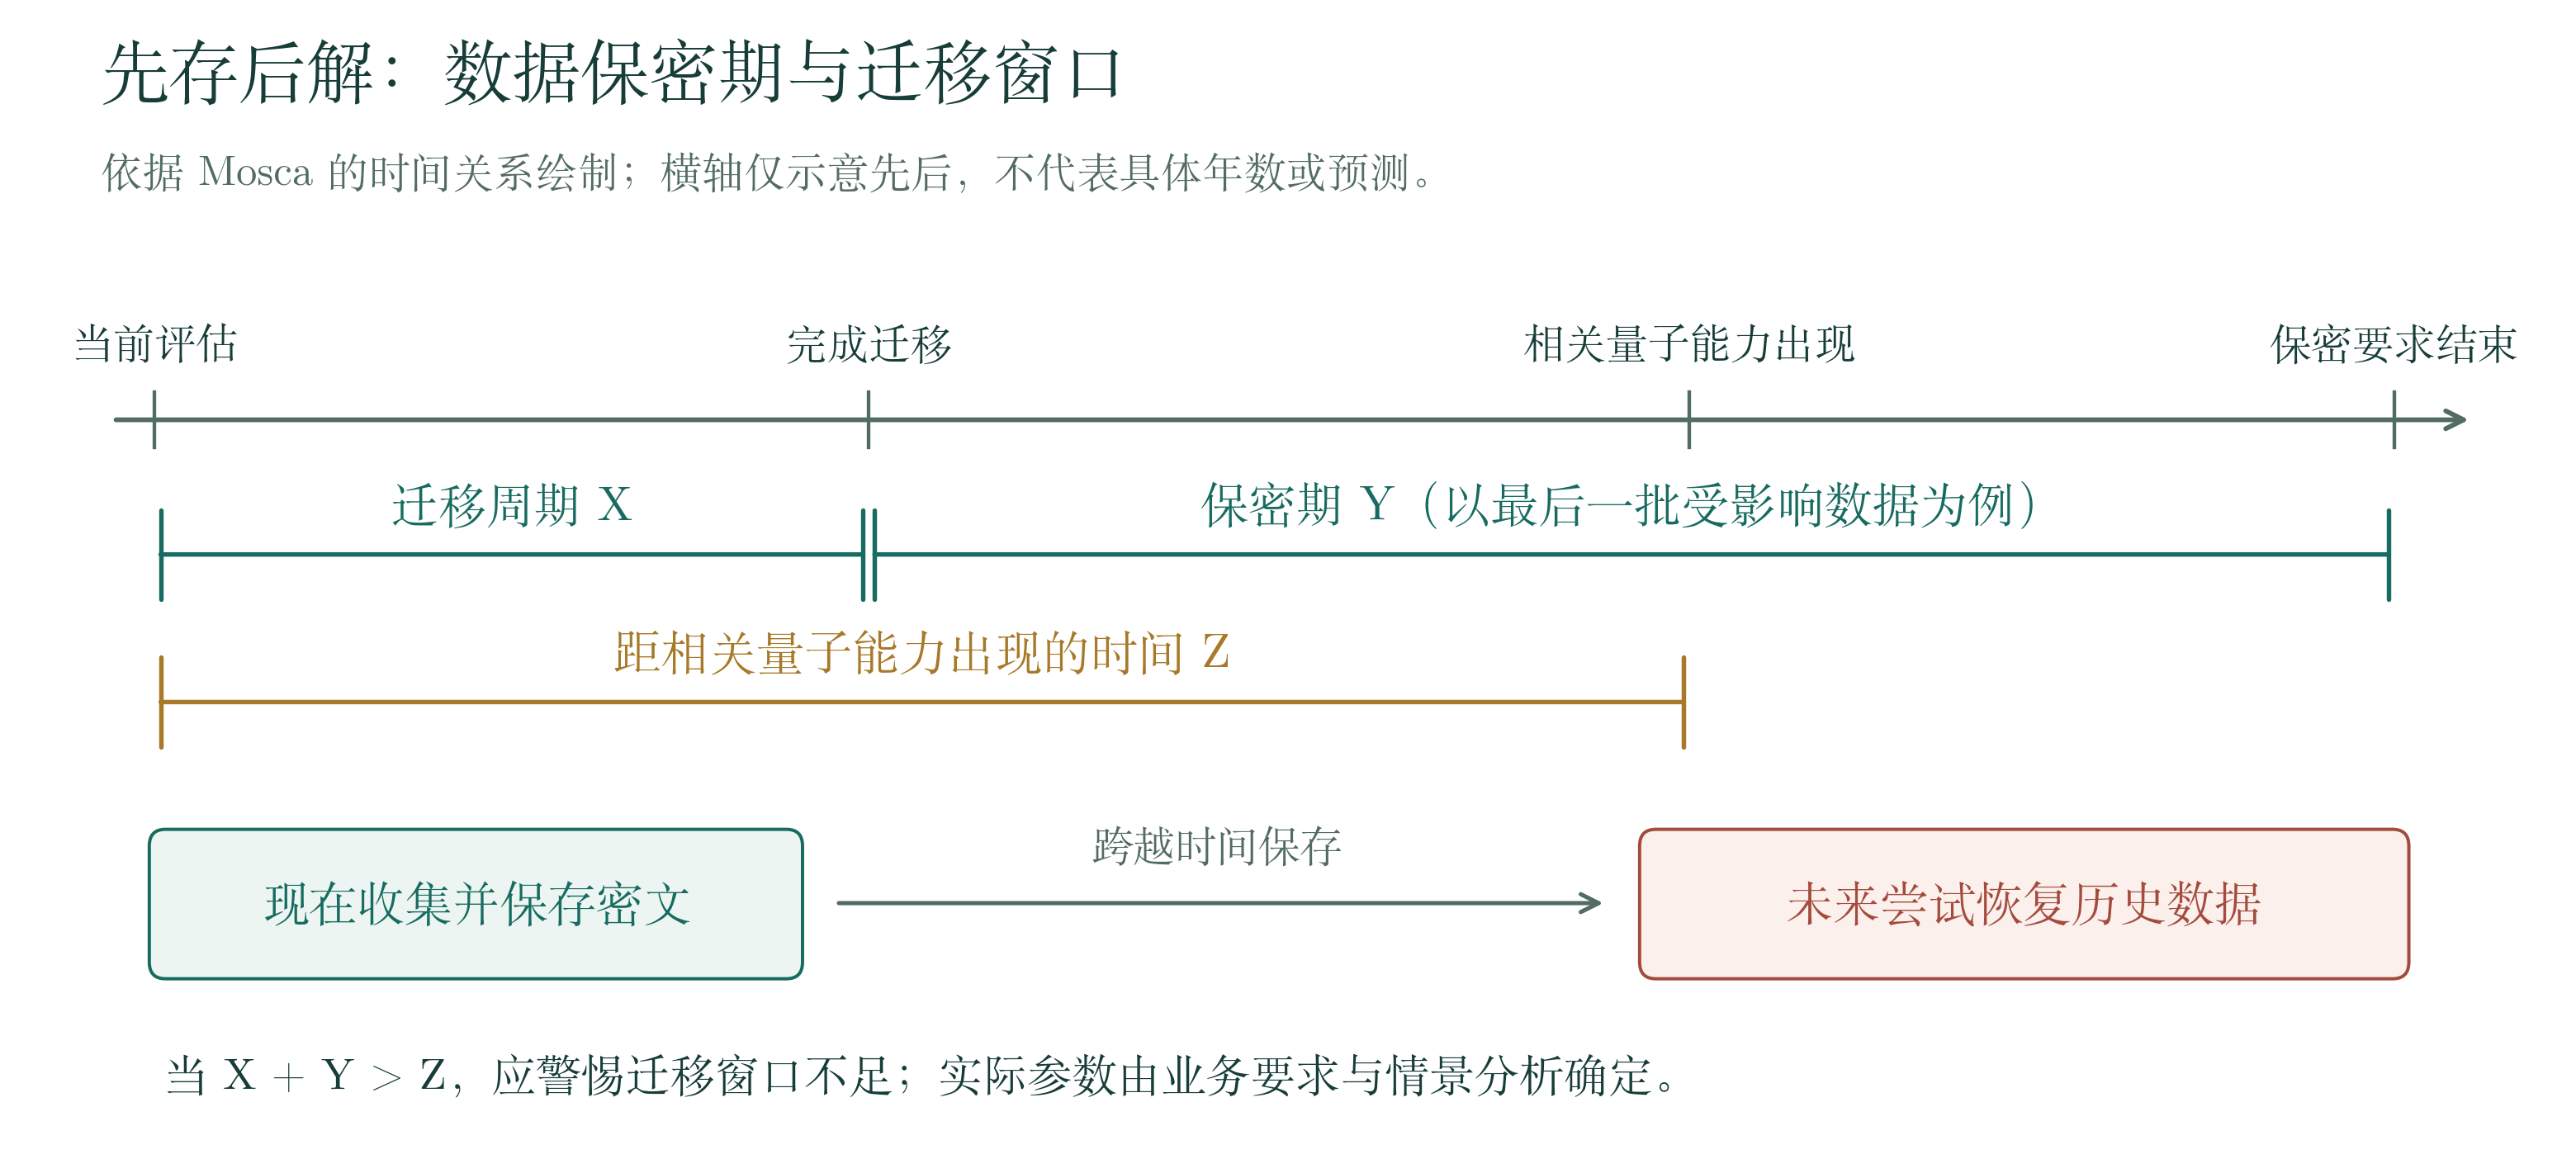
\includegraphics[width=\linewidth]{18-harvest-now-decrypt-later.png}
    \caption{先存后解的时间关系。依据 Mosca 的迁移窗口讨论绘制\cite{mosca2018}；未来量子能力的出现时点仅为示意。}
    \label{fig:gri-timeline}
\end{figure}

在工程评估中，具有指导意义的威胁模型是\textbf{先存后解}（Harvest Now, Decrypt Later，HNDL）：如图~\ref{fig:gri-timeline} 所示，攻击者现在收集并保存受影响机制保护的密文，待未来具备相关量子能力时尝试恢复历史数据。这使未来解密能力成为当前数据保护需要考虑的风险，但不表示本文已观察到实际解密损失。Mosca 提出的时间关系可用于判断迁移窗口：设 $X$ 为完成迁移所需的时间，$Y$ 为数据需要继续保持机密的年限，$Z$ 为从评估时点到相关量子能力出现的时间，若

\begin{equation}
    X + Y > Z,
    \label{eq:mosca}
\end{equation}

则需要警惕在迁移与保密要求尚未同时满足时，受影响数据已经暴露于未来解密能力的风险\cite{mosca2018}。电力系统不同业务的保密期、可升级性与检修窗口并不相同，应分别确定 $X$ 与 $Y$，并对不确定的 $Z$ 做情景分析，而不能统一指定“所有电力数据保密十至二十年”或固定的量子威胁到来日期。

为应对上述威胁，NIST 于 2024 年 8 月发布首批后量子密码标准，包括 FIPS 203（ML-KEM）、FIPS 204（ML-DSA）与 FIPS 205（SLH-DSA）\cite{nistfips203,nistfips204,nistfips205}。迁移时间安排方面，本文引用的 NIST IR 8547 为 2024 年发布的\textbf{初始公开草案}，提出对相关量子脆弱公钥算法在 2030 年前后进入弃用阶段、到 2035 年不再允许用于相应保护用途的规划\cite{nistir8547}。具体时间与范围应按算法、参数、用途及后续正式文件核对，不能表述为已经对全球电力系统生效的强制期限。IEC 62351 系列为电力系统数据与通信安全提供行业标准背景\cite{iec62351}。图~\ref{fig:pqc-timeline} 将已发布标准、草案规划节点与项目迁移活动并列展示。对我国电力行业而言，算法选用与迁移还需满足适用的商用密码制度、产品要求和业务协议约束，准确识别现有密码资产及其用途是分层迁移的前提。

% 配图说明：使用编号 PNG 的原创时间示意，标明推演条件与来源，不将示意当作实测。
\begin{figure}[htbp]
    \centering
    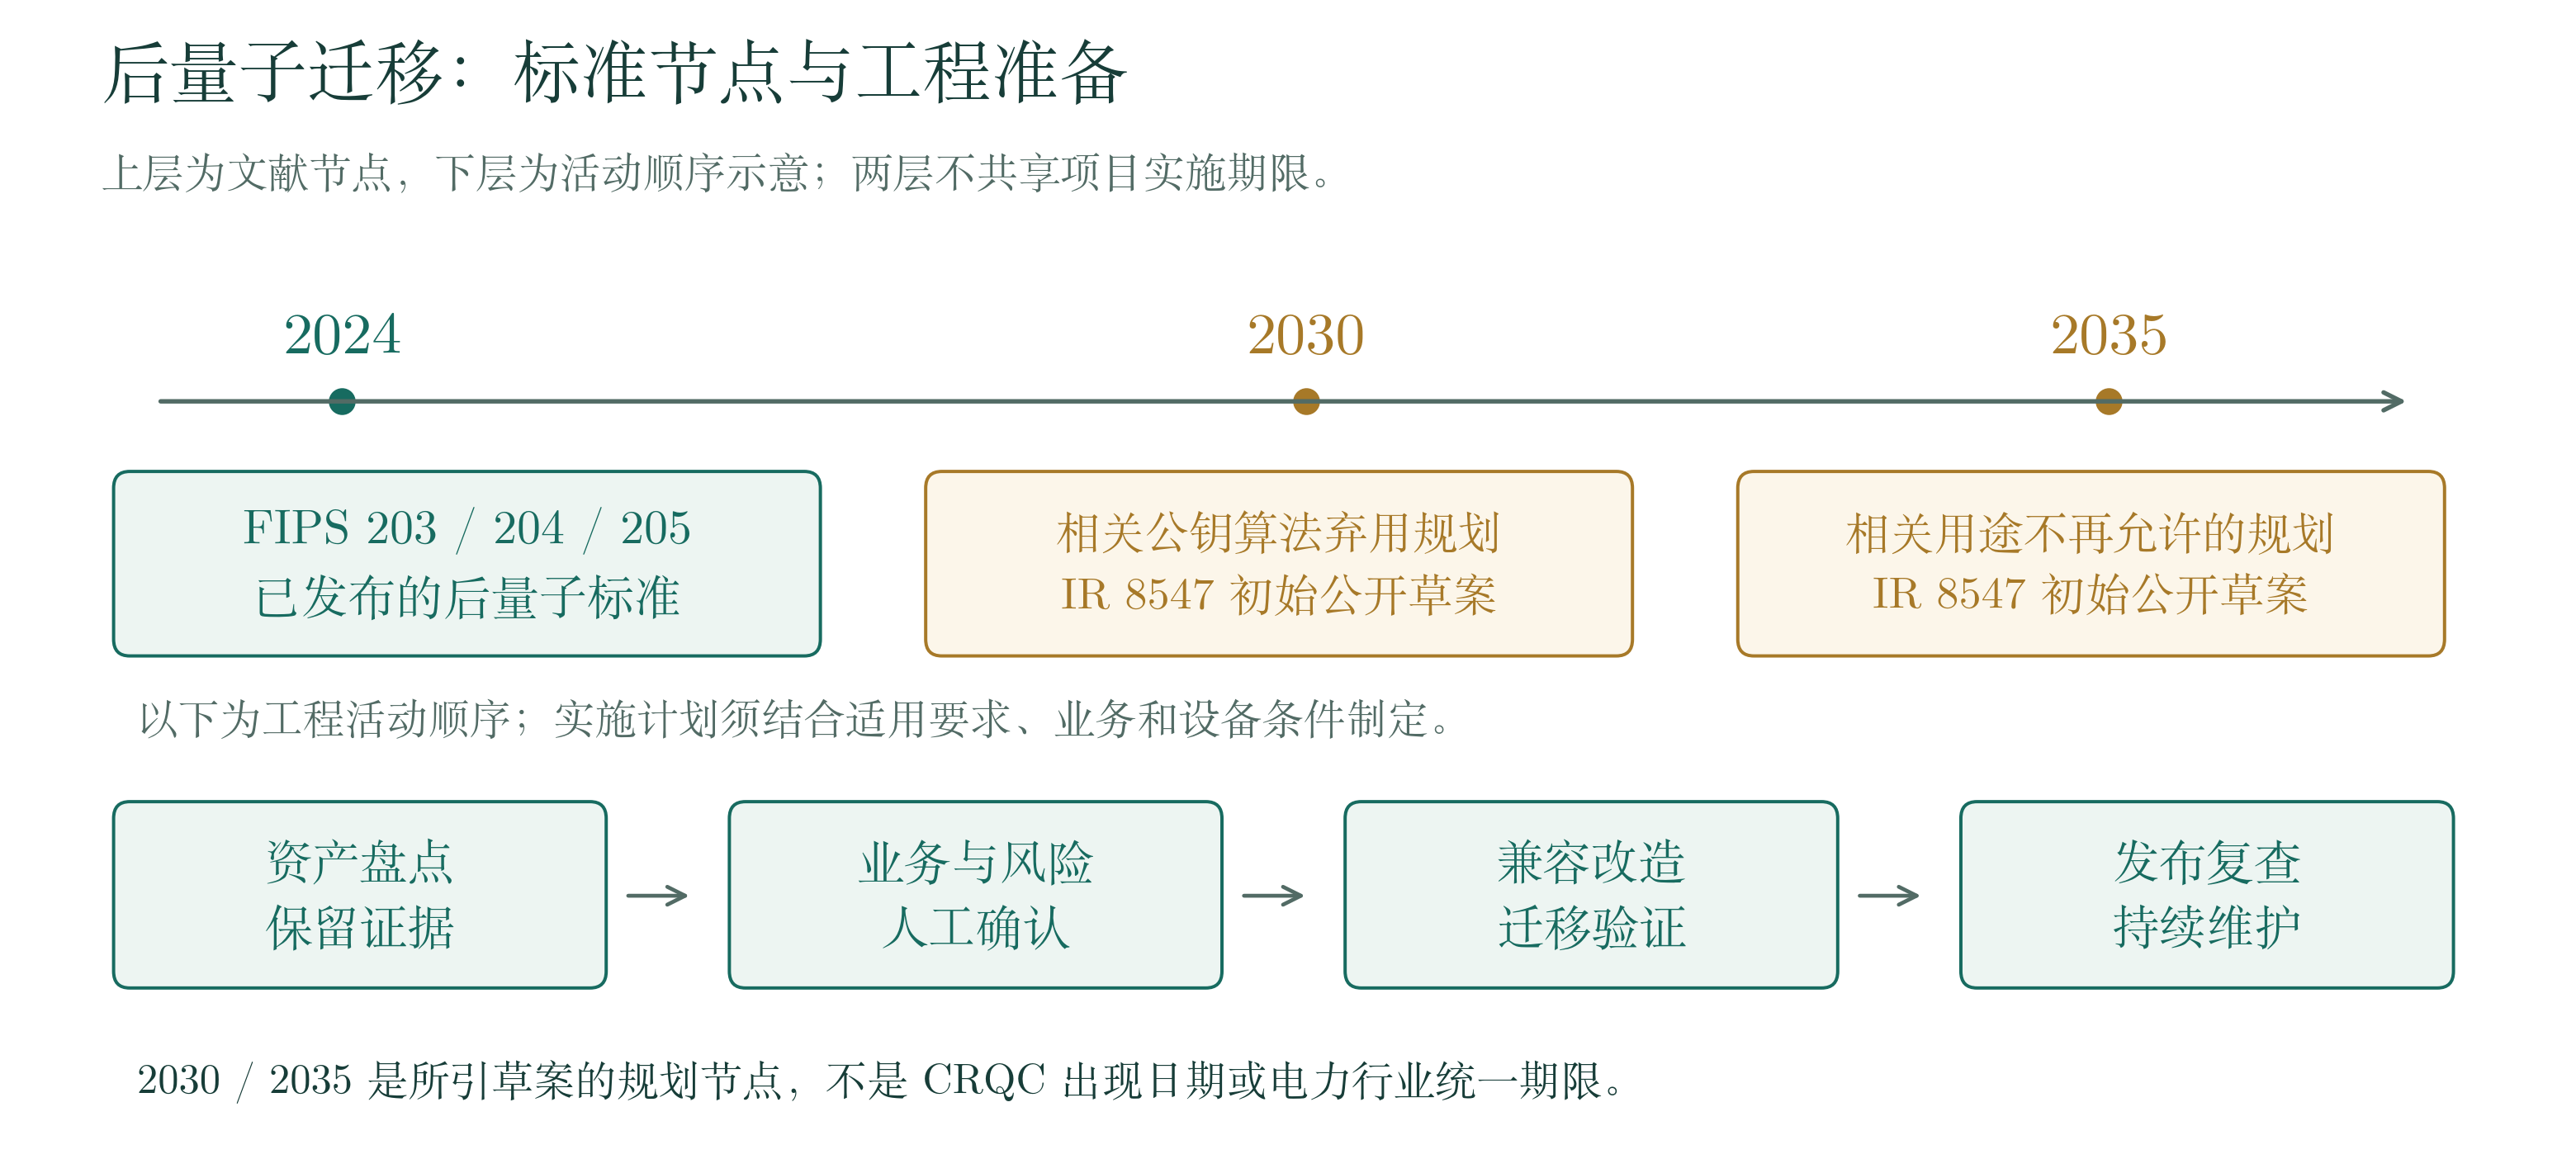
\includegraphics[width=\linewidth]{19-post-quantum-migration-timeline.png}
    \caption{后量子标准与迁移准备活动的时间关系示意。2030 与 2035 节点来自 NIST IR 8547 初始公开草案\cite{nistir8547}，不是量子计算机到来日期或电力行业统一期限。}
    \label{fig:pqc-timeline}
\end{figure}

\subsection{电力领域密码的重要性与识别的紧迫性}

电力系统是关乎国计民生的关键信息基础设施，密码技术在发电、输电、变电、配电、用电各环节深度应用，其作用不止于防止数据被窃取，还关系到控制指令真实性、软件升级可信性与电网运行稳定性。密码机制失效可能带来遥控遥调指令伪造、保护定值篡改、量测数据失真与用户信息泄露等风险。我国《电力监控系统安全防护规定》已于 2024 年修订，并自 2025 年 1 月 1 日起施行\cite{dianli27}。防护体系中的身份认证、安全传输与访问控制等环节高度依赖密码能力，因此开展资产盘点具有明确业务背景。表~\ref{tab:power-crypto-deployment} 给出各环节的典型应用形态；其中算法为业务分析示例，不代表所有实际设备采用相同配置，也不表示本文已经扫描这些现场系统。承担\textbf{身份认证与密钥分发}职能的传统公钥机制分布于多个业务链路，少量抽样难以代替系统性的资产清单与持续维护。

\begin{table}[htbp]
    \centering
    \caption{电力系统各环节的密码应用形态}
    \label{tab:power-crypto-deployment}
    \small
    \begin{tabularx}{\linewidth}{@{}p{1.9cm}p{3.4cm}p{3.0cm}X@{}}
        \toprule
        \textbf{业务环节} & \textbf{典型密码应用形态} & \textbf{涉及算法} & \textbf{迁移关注} \\
        \midrule
        调度与控制 & 纵向加密认证装置、调度数字证书系统 & SM2、RSA、SM3、SM4 & 需评估公钥迁移 \\
        \midrule
        变电站自动化 & 站控层通信安全、装置身份认证 & SM2、RSA、SM3、SM4、AES & 需评估公钥迁移 \\
        \midrule
        配电自动化 & 配电终端接入认证、遥控指令保护 & SM2、SM4 & 需评估公钥迁移 \\
        \midrule
        用电信息采集 & 采集终端安全模块、主站密钥管理 & SM4、SM2、AES & 需评估公钥迁移 \\
        \midrule
        新能源与储能 & 场站控制器通信、功率控制指令认证 & SM2、TLS 相关算法 & 需评估公钥迁移 \\
        \midrule
        运维与管理 & 运维通道 TLS/SSH、主机存储加密 & RSA、ECDSA、AES、SHA-2 & 需评估公钥迁移 \\
        \bottomrule
    \end{tabularx}
\end{table}

电力密码资产在分布上高度碎片化：终端类型至少涵盖变电站智能电子设备（IED）与测控装置、配电自动化终端（DTU/FTU/TTU）、智能电表与用电信息采集终端、纵向加密认证装置与安全接入网关、调度主站与服务器、新能源场站控制器及充电桩等；算法上既有 RSA、ECDSA、AES、SHA-2 等国际算法，也有 SM2、SM3、SM4 等国密算法，且常以混合方式并存。造成"底数不清"的技术根源有四：一是\textbf{密码与业务深度融合}，IEC 61850、DL/T 634.5104、用电信息采集等协议构成业务通信背景，其信道与管理通道可能另外部署密码安全机制\cite{iec61850,dlt634}，观察到业务流量并不等于识别出密码算法；二是\textbf{算法对上层不可见}，终端通过安全模块或安全装置提供密码能力，配置中往往只记录"启用加密"，而不记录所用算法与密钥长度；三是\textbf{多厂商、长周期的存量设备}在载体形态与实现方式上差异极大，缺乏统一的资产台账；四是\textbf{存量终端不一定具备主动上报密码配置的能力}，人工核查效率低、覆盖不全且更新滞后。上述根源共同导致电力系统的密码资产底数不清、量子脆弱性无法被全面发现，说明仅靠人工梳理难以持续支撑抗量子密码迁移这一系统性工程。

电力领域量子脆弱性识别的紧迫性来自三重因素的叠加：其一是\textbf{部分数据需要长期保密}，用户隐私、运行资料等应按业务要求评估保密期限，并据式~\eqref{eq:mosca} 分析迁移窗口；其二是\textbf{迁移周期长}，设备升级受检修窗口、备品备件、兼容性与厂商支持周期制约，需要尽早明确迁移对象与优先级；其三是\textbf{识别方式存在覆盖边界}，网络、配置和证书清点能够看到外部暴露属性，却不一定覆盖未启用功能、静态链接密码库和离线固件内部实现。由此需要形成系统性密码清单，在不干扰生产业务的条件下，结合离线证据与人工用途确认支撑迁移准备，而不能仅凭算法名称给出完整业务风险结论。

综合上述分析，本课题的目标是研制一款面向电力软件的密码资产识别与量子迁移辅助工具，实现可取得软件工件中的密码资产自动发现、算法识别与证据展示，并用组件溯源、风险提示及检测报告辅助人工分析。依据竞赛命题，作品面向四项量化目标展开：识别不少于 5 种密码算法，覆盖不少于 5 类电力终端，支持固件镜像、可执行程序等不少于 3 类检测对象，算法识别准确率不低于 90\%。本文采用有业务差异的五类终端软件场景开展验证，准确率、召回率与漏报率按明确的样本及标签口径分别报告。完整电力协议解析、自动业务风险评分、真实厂商终端与现场验证属于后续扩展方向。后续章节围绕上述目标介绍预备知识、方案设计与实验结果。

\section{国内外研究概况}

量子脆弱性识别在方法上涉及“密码资产发现”与“迁移风险分析”两个相互衔接的方向。国内外相关工作可沿三条线索梳理：密码资产发现的方法与数据表达，面向封闭软件的密码算法识别技术，以及能源行业与我国的应用要求。

\subsection{密码资产发现与迁移管理}

国际迁移实践普遍强调先发现密码使用位置，再评估影响并规划替换。NIST 国家网络安全卓越中心（NCCoE）的后量子迁移项目将\textbf{密码发现}（cryptographic discovery）作为重要工作内容，讨论通过多种发现方式构建组织范围密码清单的实践\cite{nccoe180038}。网络发现、端点与文件分析、应用与配置清点各自提供部分视图，需要保留来源和盲区。在数据表达方面，CycloneDX 1.6 引入密码学物料清单（Cryptography Bill of Materials，CBOM），为算法、协议、证书及相关密码属性提供结构化描述\cite{cbom16}。由此可形成“发现证据—结构化清单—用途确认—迁移建议”的管理链路。

工具生态既包括 IBM Quantum Safe 等企业密码发现与迁移管理方案，也包括 CBOMkit 等开源实践\cite{ibm-quantum-safe,cbomkit}。面向网络服务的发现适合了解协议和证书的外部暴露属性，源码与文件分析则有助于定位具体组件。二者不能互相替代：库内存在某种算法不表示业务已经使用，未从网络观察到某种算法也不表示发布包中不存在。本作品沿用资产发现与迁移辅助的思路，把主要工作范围放在可以取得的源码、程序与固件组件。

\subsection{封闭软件中的密码算法识别}

对于固件镜像、可执行程序等封闭对象，识别需要跨越符号缺失、编译优化与架构差异。Gr{\"o}bert、Willems 与 Holz 的研究讨论了二进制程序中密码原语的自动识别\cite{groebert2011}；2024 年 ACSAC 的系统研究进一步比较了二进制密码函数识别方法\cite{acsac24}。这些工作表明密码实现具有可分析的程序特征，也说明实验结论必须结合参考实现、构建条件与评价对象理解，不能将已知库上的识别率直接解释为未知软件的通用覆盖能力。


\paragraph{名称、字节特征与已知实现识别}
源码名称和文本关键词方法成本较低，Wind River crypto-detector 提供了相关开源实践\cite{wind-detector}。
其限制是注释、声明、普通字符串与实际调用可能包含同样的文本，因此本工具补充词法掩盖和角色判定。
YARA 适合表达常量、查表和指令片段规则\cite{yara-docs,crypto-rules}；
规则在优化、硬件加速或不同字节序下可能失效，共享常量也可能产生混淆。
已知函数签名通过覆盖完整函数、处理重定位并核对常量增强依据，
但其适用域受参考库、编译器、优化等级与架构限制。

\paragraph{结构化分析、运算语义与固件接入}
ELF/PE 结构化解析可区分导入和定义，避免把链接密码库解释为拥有库内全部算法。
Tree-sitter 提供源码语法树，Capstone 提供跨架构反汇编\cite{tree-sitter,capstone}。
本作品在上述表示上构建位运算、查表、轮函数和部分大数关系的见证，
用数据依赖约束补充名称或字节完全匹配的不足。
Unicorn 用于隔离的有限指令探针\cite{unicorn}，不是运行完整业务程序。
Miasm 提供机器语义与中间表示\cite{miasm}，但中间表达式数量并不等于完整密码算法证据。
固件提取是另一类问题：Binwalk 提供格式识别和历史提取路线\cite{binwalk-v2}，
当前工程另有原生 SquashFS、gzip 与受限 ESP 适配器，提取后复用统一扫描入口。

\begin{table}[htbp]\centering\small
\caption{主要方法的作用与限制；本表为技术比较，非同条件性能排名}\label{tab:method-comparison}
\begin{tabularx}{\linewidth}{p{2.4cm}p{4.4cm}X}\toprule
方法 & 适合解决的问题 & 主要限制\\\midrule
名称/接口 & 定位明确 API 和动态导入 & 名称可删除或变化；引用不证明实现或执行。\\
字节/常量 & 低成本定位标准表和轮常量 & 共享表、优化与字节序影响；需排除纯数据诱饵。\\
已知函数 & 核验已审核实现的完整字节与角色 & 已见库与构建覆盖有限，不能外推未知家族。\\
运算图/语义 & 识别不依赖变量名的数据依赖 & 路径、内存、调用与预算限制明显。\\
固件组件 & 把镜像关联到可定位的组件证据 & 加密区域、未知文件系统与外部硬件仍未知。\\\bottomrule
\end{tabularx}\end{table}


\subsection{能源行业与国内应用要求}

能源行业的密码迁移必须结合控制业务、安全分区、装置寿命与供应链协同。IEC 62351 系列覆盖电力数据和通信安全，IEC 61850 等标准提供业务通信背景\cite{iec62351,iec61850}。对相关系统的量子风险分析，需要把算法、证书、协议配置与实际业务用途关联起来。网络通道的安全试点或单一协议替换，都不能自动说明存量软件中全部密码能力已经完成清点。离线发布包分析可补充其中的软件证据，但不能代替装置测试与生产环境评估。

国内密码应用还受到国密算法标准与商用密码应用要求的约束。SM2、SM3、SM4 已有相应国家标准\cite{gbt32918,gbt32905,gbt32907}，GB/T 39786 与 GM/T 0054 等给出信息系统密码应用的基本要求\cite{gbt39786,gmt0054}。这类要求为身份鉴别、机密性、完整性和密钥管理等提供评估依据；后量子迁移还需要进一步考察算法的量子计算风险、替换兼容性与生命周期。满足既有合规要求与完成后量子迁移是需要分别验证的目标。

综合来看，本文重点处理三项工程问题：一是补充源码、二进制与固件之间的离线证据关联；二是区分接口引用、实现包含及尚未确认的运行时使用，避免把算法列表直接当作业务风险结论；三是在资源受限条件下，将识别证据组织为可复核资产清单，支持用途核查和迁移准备。对电力专有协议的完整解析，以及结合数据保密期、资产关键性的自动风险排序，仍需后续研究。

\clearpage
\section{作品功能与性能说明}
本作品面向电力软件交付与运维核查，由密码识别引擎、固件提取模块和本地工作台组成。用户提交文件或目录后，工具识别对象类型并执行检测，生成密码资产清单和原始证据，供用户核对密码用途、规划迁移。检测以离线静态分析为主。

源码分析支持 C/C++ 与部分 JavaScript 代码，定位密码接口调用及实现证据。程序分析面向 Linux 与 Windows 程序及共享库，记录符号和文件偏移。固件先提取内部文件，再逐组件分析并记录来源，失败或预算超限的部分单独标记。

当前支持十三种算法，包括对称加密算法 AES 和 SM4、摘要算法 SHA-256 和 SM3，以及 RSA 和 SM2 等公钥算法。智能电能表、采集集中器、馈线终端、保护装置和边缘网关五类软件样例已用于验证。十份面向两种处理器架构的自制镜像共恢复 650 个文件，其中 540 个为二进制文件，530 个文件包含密码实现，验证范围限于软件流程。

工作台可通过文件或文件夹上传、服务器路径和内置样例创建任务，查看处理阶段与历史记录，支持结果搜索和筛选。用户可核对源码行号、程序偏移及组件内容摘要，查看算法类别对应的量子风险提示与迁移建议。页面区分密码接口引用与文件内实现，局部线索留待复核，静态结果不证明实际启用。报告可导出为结构化数据、表格文件和文本，保留原始证据。命令行入口也可直接提交本地文件或目录。

既有评测使用 1071 份源码与两种架构的程序，一份文件与一种算法组成一项判定，重复证据合并计数。747 项实现标注中正确检出 726 项，漏检 21 项，没有范围内误报。计入 11206 项正确排除结果后，准确率为 99.82\%，实际存在算法的检出比例，即召回率为 97.19\%。样本参与过规则与参考库修订，结果仅说明已知实现覆盖。

耗时测量采用 Xeon Silver 4410Y 处理器、Fedora CoreOS 42 系统与 Python 3.12.3 环境，源码与程序串行测量，各类扫描均关闭可选语义后端。源码与程序沿用八份固定样本，各预运行一次再测三次；固件记录十份镜像在三个任务并发下各扫描一次的耗时，分别汇总范围。计时含进程启动、分析和报告写出，固件另含解包，不含网页交互，仅反映所测小样本表现。

\begin{table}[htbp]\centering\small
\caption{三类检测对象的文件大小与实测耗时范围}\label{tab:implemented-scope}
\begin{tabularx}{\linewidth}{@{}Xrr@{}}\toprule
检测对象 & 文件大小范围（字节） & 耗时范围（秒）\\\midrule
源码文件 & 329--1464 & 0.193--0.356\\
程序文件（共享库） & 33416--72032 & 3.012--3.884\\
固件镜像 & 3981312--4132864 & 93.208--133.740\\\bottomrule
\end{tabularx}
\end{table}

\clearpage
\section{创新性说明与优势分析}
本作品针对电力软件中密码功能分散于不同文件与组件的特点，将源码、可执行程序和固件镜像纳入统一检测流程。设计重点在于明确算法识别的判定条件，并建立识别依据与文件位置之间的对应关系，支持识别结果的定位与复核。

源码中的算法名称可能出现在注释、函数声明或调用表达式中，仅凭名称匹配难以区分其含义。本文结合词法处理与局部语法判定，区分接口名称的声明、定义与调用，将接口引用判定建立在调用及参数依据之上，并保留其在原始源码中的位置。对于通用密码接口，依据调用处明确给出的选择参数确定具体算法，参数取值无法确定时则保留待确认状态，从而减少注释及同名声明等无关文本的干扰。

对于缺少函数名称等符号信息的可执行程序，本文在 YARA 初步特征匹配\cite{yara-docs}的基础上，进一步对照固定版本开源密码库中的完整函数进行核验。核验时仅对预先审核的地址变化作匹配调整，并检查函数引用的常量及所需的关键运算。仅发现局部相似片段时，结果保留为待确认线索，满足完整核验条件后才作为算法实现的依据。匹配记录同时保留参考库版本、编译条件及核验依据，便于对照具体参考代码复查结果；匹配范围仍受已收录构建条件限制。

在程序指令分析中，本文利用 Capstone 反汇编引擎\cite{capstone}解析程序指令，并以可选的 Miasm 二进制分析框架\cite{miasm}辅助表示和分析指令中的运算关系。分析过程记录参与运算的数据来源、处理位数及前后计算关系。即使操作种类和常量相同，数据来源或计算关系不同，也可能对应不同的计算过程。保留这些信息能够区分部分表面相似的代码，为名称识别和固定代码匹配提供补充。

证据复核方面，本文将外层镜像、内部组件与算法位置建立对应关系，保留内容摘要及提取来源。软件发布包发生变化时，分析人员可据此确认发现属于哪个组件，并回到原始文件核对。复核对象由此明确到具体交付文件，便于按组件检查密码资产，其覆盖仍依赖实际提取结果。

针对多个业务系统共用密码组件时迁移影响范围难以确定的问题，本文借鉴图检索增强生成（GraphRAG）\cite{graphrag2024}的实体关系组织方法，提出结合关联图与本地大模型的扩展方案。该方案拟记录终端、业务系统与密码组件之间的使用关系，在分析组件替换或升级时，通过图检索向模型提供相关记录及依赖路径，辅助梳理可能受到影响的终端与业务。模型拟在本地部署，以减少软件代码和业务资料向外部服务传输的需求，降低敏感信息外传风险。该方案尚未完整实现，关联分析效果及运行开销仍需后续验证。

\chapter{理论基础与实验原理}\floatname{algorithm}{算法}
\renewcommand{\algorithmicrequire}{\textbf{输入：}}
\renewcommand{\algorithmicensure}{\textbf{输出：}}

\section{密码资产识别与量子风险的基本概念}
\label{sec:asset-theory}

\subsection{识别对象与证据层次}

电力终端及其他嵌入式电子设备的密码功能，可能由业务源码、
静态链接代码、动态链接库或独立密码硬件提供。
本方案实现的密码资产扫描工具记为 QCS，
面向 C/C++ 源文件、ELF/PE 程序文件和可提取文件系统的固件镜像，
分别通过词法分析、结构化符号解析、字节特征与已知函数签名获取静态证据。
固件通道将镜像内的程序和库作为组件送入同一检测流程，
使不同输入形式具有一致的算法命名和证据格式。
文本配置中的名称与库依赖也被保留，但其含义需要单独解释。

资产识别至少涉及三个层次：源码或二进制对某算法接口的静态引用、
文件中包含相应实现的静态证据，以及业务运行时实际执行该算法。
接口引用不保证实现位于当前文件；
包含实现也不保证该功能已被启用。
本工具输出前两类证据，运行时使用字段保持未知。
已审查接口的函数定义首先提供命名线索；
当前实现包含预测还要求与固定源码参考的 SHA-256 相符，
或由受限标准运算图给出已实现的依赖见证。
不能仅由函数名证明函数体具有完整、正确的密码语义。
用于评测的实现真值还需独立核对上游源码和构建配置。

当前核心评测集合为 AES、DES、RC4、ChaCha20、RSA、ECDSA、ECDH、
MD5、SHA-1、SHA-256、SM2、SM3 和 SM4，共 13 种。
模型还允许记录其他算法和算法族，
但具体输出范围取决于已审核接口与规则；
类型字典中存在某个名称不等于所有检测通道均已覆盖该算法。
Base64 单独归为编码线索，不能计为密码算法。

本工具在统一调度和证据模型中复用了
Wind River crypto-detector 的文本特征、crypto-detection 的 YARA 规则
及 Binwalk 2 的固件解包能力，
并结合结构化符号检测与自写已知函数识别
\cite{wind-detector,crypto-rules,qryx-detector,binwalk-v2}。
在此基础上，源码角色判定、规则含义映射、
整函数重定位掩码与常量约束、组件溯源及双口径评测
由本项目实现。
依赖版本、规则摘要和参考构建信息随工程保存，
作为判断报告适用范围和复现实验的依据。

共享结构是静态识别必须处理的限制。
SHA-224 与 SHA-256 复用压缩结构，BLAKE2 与 SHA-2 使用同源初始化常量，
ECDSA 与 ECDH 复用椭圆曲线点运算
\cite{rfc6234,rfc7693}。
若证据只支持共享结构，工具将其记录为候选线索，
而不把同一命中展开为多个确定算法。
本章先说明密码算法与量子威胁的理论基础，
再解释上述证据如何在当前实现中产生和组合。

\subsection{基本运算与量子风险}
\label{subsec:basic-quantum-risk}

\paragraph{基本运算与实现差异}
本文以 \(\oplus\) 表示按位异或，
以 \(\land\)、\(\lor\) 和 \(\neg\)
表示按位与、或和取反。
\(\operatorname{ROTL}_w(x,s)\) 与
\(\operatorname{ROTR}_w(x,s)\)
分别表示 \(w\) 位字的循环左移和循环右移；
逻辑右移记为 \(\operatorname{SHR}_w(x,s)\)。
对 \(0<s<w\)，有
\begin{equation}
  \operatorname{ROTL}_w(x,s)
  =
  \bigl((x\ll s)\lor(x\gg(w-s))\bigr)\bmod 2^w.
\end{equation}
同一运算可由不同指令序列实现，
常量也可能因字节序、数据宽度及编译优化而呈现不同形式。
例如，32 位常量 \(\texttt{0x6a09e667}\)
在小端表示中对应 \(\texttt{67 E6 09 6A}\)。
这些实现差异既是构造特征规则的依据，
也是漏报的重要来源。


\paragraph{量子态与测量的必要记号}
以下采用 \(\lvert x\rangle\) 表示编码整数 \(x\) 的计算基态。
量子寄存器的纯态可写为
\begin{equation}
  \lvert\psi\rangle=\sum_x\alpha_x\lvert x\rangle,
  \qquad \sum_x|\alpha_x|^2=1,
\end{equation}
其中 \(\alpha_x\) 为复数幅度；
在计算基下测量得到 \(x\) 的概率为 \(|\alpha_x|^2\)。
量子算法通过可逆运算和干涉改变这些幅度，
最终测量仍只得到一个结果。
因此，均匀叠加不意味着能够一次读出所有候选值；
有效加速需要利用问题结构或设计幅度放大过程
\cite{quantum-revisited,amplitude-amplification}。


\paragraph{Shor 算法：整数分解与量子阶寻找}
Shor 算法能够在理想量子计算模型下，
以输入比特长度的多项式规模求解整数分解和离散对数问题
\cite{shor1997}。
以整数分解为例，先对偶数、素数和素数幂进行经典预处理，
再考虑具有至少两个不同素因子的奇合数 \(N\)。
随机选取 \(a\in\{2,\ldots,N-2\}\)。
若 \(1<\gcd(a,N)<N\)，已获得非平凡因子；
否则，在 \(\gcd(a,N)=1\) 时，定义 \(a\) 模 \(N\) 的阶为
\begin{equation}
  r=\min\{t\geq1:a^t\equiv1\pmod N\}.
  \label{eq:pre-shor-order}
\end{equation}
函数 \(f(x)=a^x\bmod N\) 具有周期 \(r\)，
整数分解由此转化为阶寻找问题。

若 \(r\) 为偶数，且
\(b=a^{r/2}\bmod N\) 不等于 \(1\) 或 \(N-1\)，则
\begin{equation}
  (a^{r/2}-1)(a^{r/2}+1)\equiv0\pmod N,
\end{equation}
从而可以通过
\begin{equation}
  g_-=\gcd(b-1,N),\qquad
  g_+=\gcd(b+1,N)
  \label{eq:pre-shor-factor}
\end{equation}
提取非平凡因子。
求最大公因数和核验因子均为经典计算；
量子部分主要负责获得阶的相关信息。

为说明量子子过程，选取 \(Q=2^t\)，使
\(N^2\leq Q<2N^2\)，
并准备两个寄存器的状态
\begin{equation}
  \lvert\psi_0\rangle
  =\frac{1}{\sqrt Q}\sum_{x=0}^{Q-1}
    \lvert x\rangle\lvert0\rangle.
\end{equation}
可逆模幂电路将其变换为
\begin{equation}
  \lvert\psi_1\rangle
  =\frac{1}{\sqrt Q}\sum_{x=0}^{Q-1}
    \lvert x\rangle\lvert a^x\bmod N\rangle.
  \label{eq:pre-shor-modexp}
\end{equation}
量子傅里叶变换（Quantum Fourier Transform，QFT）定义为
\begin{equation}
  \operatorname{QFT}_Q\lvert x\rangle
  =\frac{1}{\sqrt Q}\sum_{y=0}^{Q-1}
    \exp\left(\frac{2\pi\mathrm{i}xy}{Q}\right)
    \lvert y\rangle,
\end{equation}
其中 \(\mathrm{i}^2=-1\)。
对第一寄存器施加逆 QFT 后测量得到 \(y\)，
其分布在对应于 \(y/Q\) 接近 \(j/r\) 的位置形成峰值，
其中 \(j\in\{0,\ldots,r-1\}\)。
若
\begin{equation}
  \left|\frac{y}{Q}-\frac{j}{r}\right|
  <\frac{1}{2r^2},
  \qquad \gcd(j,r)=1,
  \label{eq:pre-shor-cf}
\end{equation}
则可通过 \(y/Q\) 的连分数展开恢复分母 \(r\)。
测量并非每次都满足这些条件；
若 \(j\) 与 \(r\) 不互素，约分后的分母可能只给出阶的因子。
因此，候选分母需要经过模幂检验，
并根据结果重采样或采用进一步的经典后处理
\cite{shor1997,quantum-revisited}。

算法~\ref{alg:pre-shor-factor} 给出保留失败重试的分解流程，
其中列出了量子态制备、可逆模幂、傅里叶采样和经典后处理。
未获得通过检验的候选时，
将本次阶寻找结果标记为 \(\bot\)，继续下一次尝试。
检验 \(a^r\equiv1\pmod N\) 只能确认候选是一个周期，
并不单独证明其为最小正周期，
故最终输出仍需按式~\eqref{eq:pre-shor-factor} 核验。

\begin{algorithm}[htbp]
  \caption{基于量子阶寻找的 Shor 整数分解流程}
  \label{alg:pre-shor-factor}
  \begin{algorithmic}[1]
    \REQUIRE 已完成经典预处理的奇合数 \(N\)，尝试次数上限 \(B\)
    \ENSURE \(N\) 的非平凡因子，或未成功标记 \(\bot\)
    \STATE 选取 \(Q=2^t\)，使 \(N^2\leq Q<2N^2\)
    \FOR{\(j=1,\ldots,B\)}
      \STATE 随机选取 \(a\in\{2,\ldots,N-2\}\)
      \STATE \(g\gets\gcd(a,N)\)
      \IF{\(1<g<N\)}
        \RETURN \(g\)
      \ENDIF
      \STATE 制备双寄存器状态 \(\lvert\psi_0\rangle\)
      \STATE 执行可逆模幂，得到 \(\lvert\psi_1\rangle\)
      \STATE 对第一寄存器施加逆 QFT 并测量，得到 \(y\)
      \STATE 由 \(y/Q\) 的连分数展开恢复候选 \(r\)
      \STATE 无通过模幂检验的候选时，令 \(r\gets\bot\)
      \IF{\(r\neq\bot\)，\(r\) 为偶数，且 \(a^r\bmod N=1\)}
        \STATE \(b\gets a^{r/2}\bmod N\)
        \IF{\(b\neq1\) 且 \(b\neq N-1\)}
          \STATE \(g_-\gets\gcd(b-1,N)\)，\(g_+\gets\gcd(b+1,N)\)
          \IF{\(1<g_-<N\)}
            \RETURN \(g_-\)
          \ENDIF
          \IF{\(1<g_+<N\)}
            \RETURN \(g_+\)
          \ENDIF
        \ENDIF
      \ENDIF
    \ENDFOR
    \RETURN \(\bot\)
  \end{algorithmic}
\end{algorithm}

例如，对 \(N=15\) 和 \(a=2\)，有 \(r=4\)；
于是 \(b=4\)，
\(\gcd(4-1,15)=3\)，
\(\gcd(4+1,15)=5\)。
该例仅展示由阶到因子的数学关系，
不用于估计实际 RSA 参数的量子资源需求。


\paragraph{Shor 算法与椭圆曲线离散对数}
整数分解流程解释了 RSA 的量子脆弱性；
ECDSA 和 ECDH 则对应 Shor 算法的离散对数求解机制。
以阶为素数 \(\ell\) 的椭圆曲线子群为例，
设基点为 \(G\)，公开点为 \(Q_{\mathrm{pub}}=dG\)。
在理想群运算与傅里叶采样模型下，考察
\begin{equation}
  F(u,v)=uG+vQ_{\mathrm{pub}}=(u+dv)G,
  \qquad u,v\in\mathbb{Z}_{\ell}.
\end{equation}
对任意 \(t\in\mathbb{Z}_{\ell}\)，有
\begin{equation}
  F(u-dt,v+t)=F(u,v).
\end{equation}
这个周期方向包含未知的 \(d\)。
在函数值寄存器测量后，
对前两个寄存器进行群上的傅里叶采样，
得到的频率对 \((\alpha,\beta)\) 满足
\begin{equation}
  \beta-\alpha d\equiv0\pmod\ell.
\end{equation}
当 \(\alpha\neq0\) 时，可恢复
\begin{equation}
  d=\beta\alpha^{-1}\bmod\ell,
\end{equation}
并通过 \(dG=Q_{\mathrm{pub}}\) 核验结果。
这些关系说明离散对数求解如何利用群结构；
实际电路还需实现可逆群运算及相应的傅里叶变换
\cite{ec-shor}。

因此，RSA、ECDSA 和 ECDH 的风险来自其所依赖的困难问题
在量子模型下可被高效求解。
该结论不表示现有量子设备已经能够处理实际部署参数，
具体资源仍取决于参数规模、电路实现和纠错方案。
扩大传统 RSA 模数或椭圆曲线参数，
不能改变其困难问题受 Shor 算法影响的性质。


\paragraph{Grover 算法：无结构搜索与幅度放大}
Grover 算法用于搜索满足给定判定条件的候选值
\cite{grover1996}。
设搜索空间大小为 \(\mathcal{N}=2^\nu\)，
判定函数为 \(f:\{0,\ldots,\mathcal{N}-1\}\to\{0,1\}\)，
满足 \(f(x)=1\) 的候选共有 \(M\) 个。
量子判定过程可表示为相位查询算子
\begin{equation}
  O_f\lvert x\rangle=(-1)^{f(x)}\lvert x\rangle.
\end{equation}
该算子使目标候选的幅度变号。
初始均匀叠加态及扩散算子分别为
\begin{equation}
  \lvert s\rangle
  =\frac{1}{\sqrt{\mathcal{N}}}
    \sum_{x=0}^{\mathcal{N}-1}\lvert x\rangle,
  \qquad
  D=2\lvert s\rangle\langle s\rvert-I,
\end{equation}
其中 \(I\) 为恒等算子。
一次 Grover 迭代为 \(G=DO_f\)；
相位标记与扩散共同放大目标候选的测量概率。

当 \(0<M<\mathcal{N}\) 时，
用 \(\lvert w\rangle\) 和 \(\lvert v\rangle\)
分别表示目标候选与其余候选的归一化均匀叠加态，令
\begin{equation}
  \sin^2\theta=\frac{M}{\mathcal{N}},
  \qquad 0<\theta<\frac{\pi}{2}.
\end{equation}
初始态满足
\begin{equation}
  \lvert s\rangle
  =\sin\theta\,\lvert w\rangle
   +\cos\theta\,\lvert v\rangle.
\end{equation}
在这两个态张成的子空间中，
每次迭代使状态朝目标方向旋转 \(2\theta\)。
执行 \(t\) 次迭代后，有
\begin{equation}
  G^t\lvert s\rangle
  =\sin((2t+1)\theta)\lvert w\rangle
   +\cos((2t+1)\theta)\lvert v\rangle,
\end{equation}
因此成功概率为
\begin{equation}
  P_t=\sin^2((2t+1)\theta).
  \label{eq:pre-grover-probability}
\end{equation}
该概率随迭代次数振荡，
故迭代次数应与目标候选比例相匹配。
当 \(M/\mathcal{N}\) 很小时，取接近首次概率峰值的次数，有
\begin{equation}
  t_\ast\approx\frac{\pi}{4}
  \sqrt{\frac{\mathcal{N}}{M}},
  \qquad
  Q_{\mathrm{Grover}}
  =\mathcal{O}\!\left(\sqrt{\frac{\mathcal{N}}{M}}\right)
  \label{eq:pre-grover-complexity}
\end{equation}
的查询数量级\cite{amplitude-amplification}。

算法~\ref{alg:pre-grover-search}
给出 \(M\) 已知且 \(1\leq M\leq\mathcal{N}/2\) 时的基本流程。
若 \(M\) 未知，需要采用迭代次数搜索或估计策略，
不能直接使用依赖 \(M\) 的次数公式。
测量得到的候选仍应进行经典核验。

\begin{algorithm}[htbp]
  \caption{目标数量已知时的 Grover 搜索流程}
  \label{alg:pre-grover-search}
  \begin{algorithmic}[1]
    \REQUIRE 搜索空间大小 \(\mathcal{N}=2^\nu\)，
             判定函数 \(f\)，目标数量 \(1\leq M\leq\mathcal{N}/2\)
    \ENSURE 满足条件的候选，或本次未成功标记 \(\bot\)
    \STATE 准备均匀叠加态 \(\lvert s\rangle\)
    \STATE \(\theta\gets\arcsin\sqrt{M/\mathcal{N}}\)
    \STATE \(t_\ast\gets\lfloor\pi/(4\theta)\rfloor\)
    \FOR{\(j=1,\ldots,t_\ast\)}
      \STATE 施加相位查询算子 \(O_f\)
      \STATE 施加扩散算子 \(D\)
    \ENDFOR
    \STATE 在计算基下测量，得到候选 \(x\)
    \IF{\(f(x)=1\)}
      \RETURN \(x\)
    \ELSE
      \RETURN \(\bot\)
    \ENDIF
  \end{algorithmic}
\end{algorithm}


\paragraph{密码搜索模型与风险解释边界}
对于对称密码的通用密钥搜索，
可将已知明密文对 \((P_i,C_i)\) 构成的验证条件写为
\begin{equation}
  f(K)=
  \begin{cases}
    1, & \text{对所有 }i,\ E_K(P_i)=C_i,\\
    0, & \text{其他情况}.
  \end{cases}
\end{equation}
其中 \(E_K\) 表示在候选密钥 \(K\) 下的加密运算。
在密钥均匀随机、验证信息足以排除错误候选，
且候选验证可实现为相应量子电路的理想模型下，
对 \(k\) 位密钥可令 \(\mathcal{N}=2^k\) 且 \(M=1\)。
按候选验证次数计，有
\begin{equation}
  Q_{\mathrm{classical}}=\mathcal{O}(2^k),
  \qquad
  Q_{\mathrm{Grover}}=\mathcal{O}(2^{k/2}).
\end{equation}
如果存在多个通过验证的候选，
则应使用式~\eqref{eq:pre-grover-complexity}
中的 \(M\)，并增加验证信息以确认目标密钥。

相位查询算子需要可逆地实现密码运算、结果比较，
并通过反计算清除辅助状态。
查询次数没有包含这些电路的全部资源开销。
若一次相位查询和扩散的逻辑门成本分别为
\(C_{O_f}\) 与 \(C_D\)，
则一次搜索的门成本可概略写为
\begin{equation}
  C_{\mathrm{total}}
  \approx C_{\mathrm{prep}}
         +t_\ast(C_{O_f}+C_D),
\end{equation}
其中 \(C_{\mathrm{prep}}\) 为状态准备成本。
该表达式仍未包含物理纠错、设备时钟、
并行化安排和失败重试等成本，
不能直接换算为实际攻击时间\cite{pqc-faq}。

对于理想 \(n\) 位摘要，固定目标摘要并搜索其原像时，
若候选空间中满足目标条件的比例约为 \(2^{-n}\)，
Grover 搜索对应
\(\mathcal{O}(2^{n/2})\) 的查询数量级。
碰撞搜索则要求寻找任意两个不同输入
\(x\neq x'\)，使 \(H(x)=H(x')\)，
与固定摘要的原像搜索具有不同目标，
不能直接使用同一公式评价。
此外，MD5、SHA-1 等算法的已有经典缺陷
仍应按用途独立纳入判断。

据此，密码资产的量子风险评估应区分
困难问题可被 Shor 算法高效求解的公钥机制，
以及受到 Grover 通用搜索影响的对称密码和原像搜索任务。
这些理论结论需要与算法参数、实际用途、
实现位置和业务依赖共同解释，
不能仅凭静态规则命中判断系统已经失去保护能力。
QCS 并未执行量子算法、量子资源估计、自动风险评分或密码迁移。
下文迁移建议属于资产核实之后的理论讨论与处置原则，
需在用途和参数得到核实后应用；
对电力终端，还应验证协议兼容性、处理时延、
存储资源、密钥更新及适用的密码使用要求。


\section{密码算法的结构、识别依据与迁移考虑}

\subsection{AES}
\label{subsec:pre-aes}

\paragraph{算法结构与用途}

高级加密标准（Advanced Encryption Standard，AES）是分组密码，分组长度为 128 位，密钥长度为 128、192 或 256 位，对应 10、12 或 14 轮变换\cite{fips197}。AES 的轮结构包含字节代换、行移位、列混合和轮密钥加，最后一轮省略列混合。其中字节代换采用固定 S 盒，列混合在有限域 \(\mathrm{GF}(2^8)\) 上运算，
其约简多项式为
\begin{equation}
  m(x)=x^8+x^4+x^3+x+1.
\end{equation}

软件实现可使用 S 盒、合并变换的 T 表或处理器专用指令。AES 可作为通信与存储保护的基础组件；机密性和认证能力还取决于工作模式及协议设计。

\paragraph{静态识别依据与边界}

本工具通过明确的 AES 接口、结构化符号以及 S 盒、T 表和指令模式
识别 AES 相关资产。
其中 \nolinkurl{RijnDael_AES_CHAR} 描述 S 盒前 32 字节，
起始片段为 \(\texttt{63 7C 77 7B F2 6B 6F C5}\)；
其他已审核规则描述逆 S 盒、合并查找表和密钥扩展常量。
轮常量前十项为
\begin{equation}
\operatorname{Rcon}=(\texttt{01},\texttt{02},\texttt{04},\texttt{08},\texttt{10},
\texttt{20},\texttt{40},\texttt{80},\texttt{1B},\texttt{36}).
\end{equation}
\nolinkurl{AES_bytecode_AESNI_x64} 提供 AES 专用指令的字节证据，
只有对象架构确认为 x86-64 时才按相应指令规则解释。
源码中的直接选择器还能将明确的 AES 模式名称或枚举与通用接口关联。
这些证据不自动给出密钥长度、工作模式或业务调用关系；
运行时生成表、位切片实现和未覆盖硬件指令仍可能导致漏检。
查找表也可能作为数据保存在文件中，因此常量命中的结论仍是静态实现线索。

\paragraph{风险与迁移考虑}

Grover 搜索改变通用密钥搜索的理论数量级，
但不等同于 AES 已被实际攻破。
NIST 的量子密码常见问题说明，
现有应用可继续使用 128、192、256 位 AES\cite{pqc-faq}。
对于长期保密且资源条件允许的业务，
可评估 AES-256，
同时核实工作模式、密钥来源和随机数或计数器管理。
需要机密性与完整性共同保护时，
可评估协议支持的认证加密方案，
而不能仅通过增加 AES 密钥长度
弥补缺少认证的设计。


\subsection{DES}
\label{subsec:pre-des}

\paragraph{算法结构与用途}

数据加密标准（Data Encryption Standard，DES）
采用 16 轮 Feistel 结构，
分组长度为 64 位，有效密钥长度为 56 位；
通常表示为 64 位的密钥
包含 8 位奇偶校验位\cite{fips46}。
初始置换后的状态分为 \(L_0,R_0\)，
第 \(i\) 轮满足
\begin{equation}
  L_i=R_{i-1},
  \qquad
  R_i=L_{i-1}\oplus f(R_{i-1},K_i),
  \quad 1\leq i\leq16.
\end{equation}
轮函数包括扩展置换、子密钥异或、
S 盒代换及 P 置换。
识别 DES 有助于定位遗留密码组件，
但其存在不说明电力业务仍在启用该组件。

\paragraph{静态识别依据与边界}

DES 的初始置换、末置换、扩展表、S 盒与密钥置换表，
为常量扫描提供结构依据；SP 表还可反映合并 S 盒与 P 置换的优化实现。
本工具保留相应规则名、匹配偏移和字节，
但不把表片段匹配等同于验证完整的 16 轮运算。
由于 TDEA 复用 DES 基础组件，共享表和运算模式只形成 DES/3DES 候选。
明确区分单 DES 与 TDEA，需要算法专用接口或其他独立证据。
本工具的接口映射可记录这类区别；无法区分的共享规则仍留在候选集合中。
表布局、编译器与等价位操作的变化会影响字节特征覆盖。

\paragraph{风险与迁移考虑}

单 DES 的 56 位密钥
已不足以满足现代安全需求，
其迁移具有明确的经典安全依据。
此外，64 位分组在相关工作模式下
存在随数据量增长的生日界限制，
该问题与密钥搜索应分别评估。
TDEA 不宜作为长期升级目标：
NIST 已于 2024 年撤销 SP 800-67 Rev.~2
\cite{sp80067}。
对确认启用 DES 或 TDEA 的业务，
应评估迁往适用的现代分组密码及认证保护方案，
并安排存量密文处理、密钥轮换
和新旧协议互操作验证。


\subsection{RC4}
\label{subsec:pre-rc4}

\paragraph{算法结构与用途}

RC4 是字节级流密码，
由密钥调度算法（KSA）
和伪随机生成算法（PRGA）组成。
KSA 将 \(S\) 初始化为 \(0,\ldots,255\) 的排列，
再按密钥字节更新索引并交换数组元素\cite{rc4-ksa}。
设密钥字节数为 \(\ell>0\)，
则其主要更新为
\begin{equation}
  j\leftarrow(j+S[i]+K[i\bmod\ell])\bmod256,
  \qquad
  \operatorname{swap}(S[i],S[j]).
\end{equation}
PRGA 继续更新排列并生成密钥流，
明文与密钥流异或得到密文。
该结构解释了初始化循环的 256 次迭代
及字节取模操作。

\paragraph{静态识别依据与边界}

RC4 的状态初始化和 256 次循环可以形成扫描特征，
但相同比较常量也大量出现在普通数组处理程序中。
本工具将仅匹配 255、256 比较或一般初始化循环的规则降为弱线索，
不会据此确认存在 RC4 的排列交换和密钥流生成。
明确的 RC4 接口引用与已定义符号具有不同的证据角色，
分别计入静态引用和实现包含口径。
没有符号且未满足专用特征的实现仍可能漏检，
人工核实时应检查索引更新、交换操作和 PRGA 数据关系。

\paragraph{风险与迁移考虑}

RC4 的密钥流偏差构成经典安全问题，
RFC 7465 已禁止在 TLS 中
协商 RC4 套件\cite{rfc7465}。
确认启用 RC4 的通信业务应优先评估替换；
协议允许时，可选择 AES-GCM
或 ChaCha20-Poly1305 等认证加密方案。
扩大 RC4 密钥长度不能消除其结构性偏差，
迁移时还应同时更新套件协商、
密钥管理及报文认证机制。


\subsection{ChaCha：以 ChaCha20 为例}
\label{subsec:pre-chacha}

\paragraph{算法结构与用途}

ChaCha 采用模加、循环移位与异或组成的 ARX 结构。
RFC 8439 定义的 ChaCha20
使用 256 位密钥、96 位 nonce 和 32 位分组计数器，
通过 20 轮变换生成密钥流\cite{rfc8439}。
内部状态为 16 个 32 位字，
列轮与对角轮交替执行。
其四分之一轮如下；
所有加法均按模 \(2^{32}\) 计算。

\begin{algorithm}[htbp]
  \caption{ChaCha 的四分之一轮}
  \label{alg:chacha-quarter-round}
  \begin{algorithmic}[1]
    \REQUIRE 四个 32 位状态字 \(a,b,c,d\)
    \STATE \(a\gets(a+b)\bmod2^{32}\);
           \(d\gets\operatorname{ROTL}_{32}(d\oplus a,16)\)
    \STATE \(c\gets(c+d)\bmod2^{32}\);
           \(b\gets\operatorname{ROTL}_{32}(b\oplus c,12)\)
    \STATE \(a\gets(a+b)\bmod2^{32}\);
           \(d\gets\operatorname{ROTL}_{32}(d\oplus a,8)\)
    \STATE \(c\gets(c+d)\bmod2^{32}\);
           \(b\gets\operatorname{ROTL}_{32}(b\oplus c,7)\)
    \ENSURE 更新后的 \(a,b,c,d\)
  \end{algorithmic}
\end{algorithm}

\paragraph{静态识别依据与边界}

初始化字符串 \texttt{expand 32-byte k}、
以及循环移位量 16、12、8、7，可以提供 ARX 结构线索。
然而初始化常量与 Salsa20 共享，
四分之一轮本身也不能说明总轮数为 20。
因此，本工具将共享常量和未充分区分轮数的指令特征保留为候选，
通过明确的 ChaCha20 接口与符号形成算法级发现。
指令字节规则还受到目标架构限制。
ChaCha20 的发现不能自动推出采用了 Poly1305、满足 nonce 唯一性，
或使用了标准规定的计数器与消息格式。

\paragraph{风险与迁移考虑}

对标准 ChaCha20，
可使用通用密钥搜索模型讨论量子影响，
但不能将其归为受 Shor 算法直接破解的公钥算法。
工程检查应核实同一密钥下 nonce 的唯一性、
计数器边界及密钥质量。
单独 ChaCha20 提供加密功能；
需要认证时，应使用协议定义的
ChaCha20-Poly1305 等完整构造\cite{rfc8439}。
仅因扫描发现 ChaCha 特征，
不足以提出更换算法的结论。


\subsection{RSA}
\label{subsec:pre-rsa}

\paragraph{算法结构与用途}
RSA 是可用于构造公钥加密和数字签名方案的传统公钥算法。
以双素数 RSA 为例，选取不同的奇素数 \(p,q\)，令
\begin{equation}
  N=pq,\qquad
  \lambda(N)=\operatorname{lcm}(p-1,q-1).
\end{equation}
公钥由模数 \(N\) 和指数 \(e\) 构成，其中
\(3\leq e<N\) 且 \(\gcd(e,\lambda(N))=1\)；
私钥指数 \(d\) 满足
\begin{equation}
  ed\equiv1\pmod{\lambda(N)}.
\end{equation}
RSA 的加密与解密原语可写为
\begin{equation}
  c=m^e\bmod N,\qquad m=c^d\bmod N,
  \qquad 0\leq m<N.
  \label{eq:pre-rsa-primitive}
\end{equation}
这里的 \(m\) 是经过规定编码后得到的整数表示。
实际加密方案还包含消息编码、随机化和解码检查，
例如 RSAES-OAEP；签名方案则使用相应的摘要编码和验证过程，
例如 RSASSA-PSS。
因此，式~\eqref{eq:pre-rsa-primitive} 仅说明模幂原语，
完整方案应按其编码与验证规则实现\cite{rfc8017}。

在电力终端的密码资产分析中，RSA 可对应证书签名、
身份认证、软件或固件签名验证，以及采用 RSA 密钥传输的遗留协议等用途。
上述用途是否存在于具体终端，需要由程序接口、配置和业务调用关系确认。
同一终端包含 RSA 实现，并不意味着上述功能均已启用。

\paragraph{静态识别依据与边界}

RSA 专用加解密、签名或验签接口可提供算法身份依据，
如 \nolinkurl{mbedtls_rsa_rsaes_oaep_encrypt} 与
\nolinkurl{mbedtls_rsa_rsassa_pss_sign}\cite{mbedtls-source}。
源码中的调用、定义和声明由不同角色记录；
ELF 的 \nolinkurl{.symtab}、\nolinkurl{.dynsym} 以及 PE 导入表
提供结构化的定义或外部引用证据。
对支持的无符号 ELF，
本工具还可识别选定 Mbed TLS 参考构建中的完整 RSA 运算函数，
其证据属于实现包含，不属于运行时调用确认。

OpenSSL 的 \nolinkurl{EVP_PKEY_encrypt} 是通用公钥接口
\cite{openssl-pkey-encrypt}，
单独出现该接口、\nolinkurl{libcrypto} 依赖或大整数模幂，
均不足以确认 RSA。
源码中直接可见的 RSA 类型选择器可以补充身份依据；
跨函数传播、动态选择、未知库版本、内联与未覆盖编译配置仍可能造成漏检。

\paragraph{风险与迁移考虑}
足够规模的容错量子计算机可利用 Shor 算法分解 RSA 模数，
并据此恢复私钥所需的参数\cite{shor1997}。
增大模数可以改变具体计算成本，但不能将 RSA 转变为抗量子方案。
风险判断还需要区分加密与签名用途：
长期保密数据涉及密文的持续保密要求，
证书或固件签名涉及身份信任和验证机制的持续有效性。

迁移候选应按功能分别选择。
对密钥建立用途，可评估 ML-KEM 等密钥封装机制；
对签名用途，可评估 ML-DSA 或 SLH-DSA 等后量子签名方案
\cite{nistfips203,nistfips204,nistfips205}。
这些方案具有不同的接口和数据格式，需重新验证协议消息、
证书标识、密钥管理、签名验证链及终端资源消耗。
当 RSA 用于固件验证时，还需核实设备的信任根和启动验证组件能否升级。
仅替换业务程序中的算法名称，不能完成上述迁移。


\subsection{ECDSA}
\label{subsec:pre-ecdsa}

\paragraph{算法结构与用途}
椭圆曲线数字签名算法
（Elliptic Curve Digital Signature Algorithm，ECDSA）
用于签名和验签，其数学基础涉及椭圆曲线离散对数问题。
为说明基本运算，本节采用素域上的短 Weierstrass 曲线
\begin{equation}
  E:\ y^2=x^3+ax+b\pmod p,
  \qquad 4a^3+27b^2\not\equiv0\pmod p,
\end{equation}
其中 \(p>3\) 为素数。
选取阶为素数 \(n\) 的基点 \(G\)，
私钥为 \(d\in\{1,\ldots,n-1\}\)，公钥为
\begin{equation}
  Q=dG.
\end{equation}
点乘 \(dG\) 表示椭圆曲线群上的标量乘法，而非坐标的普通数乘。

设 \(z\) 为按规范由消息摘要转换得到的整数。
签名端选取本次签名使用的秘密值 \(k\)，计算
\begin{equation}
  R=kG,\qquad
  r=x(R)\bmod n,\qquad
  s=k^{-1}(z+rd)\bmod n.
  \label{eq:pre-ecdsa-sign}
\end{equation}
对采用随机秘密值的过程，若 \(r=0\) 或 \(s=0\)，应重新选取 \(k\)。
摘要的整数转换需遵循所选规范；
例如 FIPS 186-5 根据子群阶的位长截取摘要的最左侧比特，
再转换为整数\cite{fips1865}。
本次签名秘密值的生成也可采用协议与实现支持的确定性方式，
RFC 6979 给出了相关构造\cite{rfc6979}。

在域参数和公钥已通过适用验证的前提下，
验签过程可概括为算法~\ref{alg:pre-ecdsa-verify}。
其判定依赖消息摘要、签名、公钥和域参数的共同参与；
签名长度或曲线名称只能提供辅助线索。

\begin{algorithm}[htbp]
  \caption{ECDSA 签名验证的基本过程}
  \label{alg:pre-ecdsa-verify}
  \begin{algorithmic}[1]
    \REQUIRE 消息 \(M\)，签名 \((r,s)\)，已验证的域参数及公钥 \(Q\)
    \ENSURE 接受或拒绝签名
    \IF{\(r\notin\{1,\ldots,n-1\}\) 或 \(s\notin\{1,\ldots,n-1\}\)}
      \STATE 拒绝并终止
    \ENDIF
    \STATE 按所选规范将 \(H(M)\) 转换为整数 \(z\)
    \STATE \(w\gets s^{-1}\bmod n\)
    \STATE \(u_1\gets zw\bmod n,\quad u_2\gets rw\bmod n\)
    \STATE \(R'\gets u_1G+u_2Q\)
    \IF{\(R'=\mathcal{O}\)}
      \STATE 拒绝并终止
    \ENDIF
    \STATE 当且仅当 \(x(R')\bmod n=r\) 时接受
  \end{algorithmic}
\end{algorithm}

其中 \(\mathcal{O}\) 表示椭圆曲线群的单位元。
该伪代码用于说明核心数学判定，
实际实现还需检查编码、域参数、公钥和所选摘要函数等条件
\cite{fips1865}。

\paragraph{静态识别依据与边界}

本工具依据专用接口与结构化符号识别 ECDSA。
Mbed TLS 的签名入口为 \nolinkurl{mbedtls_ecdsa_sign}，
验签入口为 \nolinkurl{mbedtls_ecdsa_verify}\cite{mbedtls-source}。
对于已纳入参考库的无符号 ELF，
可由 TinyCrypt 或 micro-ecc 的完整签名、验签函数提供实现证据。
这类匹配保留算法操作函数的完整字节约束与参考构建来源，
不以通用椭圆曲线点乘函数替代签名功能判别。

\nolinkurl{EC_KEY_generate_key}、\nolinkurl{mbedtls_ecp_mul} 和
通用 \nolinkurl{EC_*} 符号仅构成椭圆曲线相关线索。
曲线参数也不能区分签名和密钥协商。
识别到签名接口不证明证书或固件更新实际使用了该接口，
也不能判断签名秘密值生成是否安全。
包装调用、未知实现、符号删除与函数内联可能影响各检测通道，
需通过不同构建条件的独立样本检验覆盖范围。

\paragraph{风险与迁移考虑}
Shor 算法能够在相应量子计算模型下求解椭圆曲线离散对数，
从公开点 \(Q=dG\) 恢复秘密标量 \(d\)，
因而威胁 ECDSA 的签名密钥\cite{ec-shor}。
更换为更大参数的传统椭圆曲线，会改变计算资源需求，
但仍保留相同类型的量子脆弱性。

ECDSA 还需要独立关注每次签名秘密值 \(k\) 的保护；
重复使用或泄露该值可能导致私钥恢复。
这属于实现与随机数管理问题，
应与量子计算造成的算法层面风险分别评价。
仅发现 ECDSA 接口，并不足以判断其秘密值生成是否存在缺陷。

迁移时，可按协议和信任体系要求评估
ML-DSA 或 SLH-DSA 等后量子签名方案\cite{nistfips204,nistfips205}。
对采用数字签名的终端证书、软件包或固件更新，
应验证公钥与签名格式、证书算法标识、验证端兼容性和信任根更新流程。
代码体积、验证时延、工作内存及签名传输开销需要在目标终端上测量，
不能只依据算法名称作出迁移结论。


\subsection{ECDH}
\label{subsec:pre-ecdh}

\paragraph{算法结构与用途}
椭圆曲线 Diffie--Hellman
（Elliptic Curve Diffie--Hellman，ECDH）
是一种密钥协商机制，用于在双方之间建立共享秘密。
沿用前节的曲线群和基点 \(G\)，
双方分别选取私钥 \(d_A,d_B\)，公开
\begin{equation}
  Q_A=d_AG,\qquad Q_B=d_BG.
\end{equation}
在对方公钥和域参数满足适用要求时，双方计算
\begin{equation}
  Z_A=d_AQ_B,\qquad Z_B=d_BQ_A.
\end{equation}
由标量乘法的性质，有
\begin{equation}
  Z_A=d_Ad_BG=d_Bd_AG=Z_B.
  \label{eq:pre-ecdh-shared}
\end{equation}
该等式解释了双方获得相同共享点的原因。
实际协议通常按规定编码提取共享秘密，
再通过密钥派生函数得到会话密钥。
其过程可抽象为
\begin{equation}
  K=\operatorname{KDF}\bigl(\operatorname{Encode}(Z),
                           \mathrm{Context},L\bigr),
\end{equation}
其中 \(L\) 为派生长度，\(\mathrm{Context}\) 为协议规定的上下文。
编码和派生方式应遵循所采用的协议，
并完成公钥验证、身份绑定及必要的密钥确认\cite{sp80056a}。

ECDH 的输出可供后续对称加密或认证机制使用，
而业务数据的加密由相应对称方案完成。
ECDH 本身不建立通信对方的身份真实性；
身份鉴别需要由证书签名、预共享认证信息等协议机制提供。
使用临时密钥对的 ECDHE，
在具备适当身份认证并销毁临时秘密等条件下，
可提供针对随后长期密钥泄露的前向保密属性\cite{rfc8446}。

\paragraph{静态识别依据与边界}

ECDH 识别关注共享秘密计算与协商操作，
如 \nolinkurl{mbedtls_ecdh_compute_shared} 和
\nolinkurl{mbedtls_ecdh_calc_secret}\cite{mbedtls-source}。
本工具分别记录源码调用、符号引用与定义，
并在受支持的无符号 ELF 中识别已知 TinyCrypt、micro-ecc 协商函数。
通用点乘、曲线参数和库依赖仍保持为候选，
不会同时展开为 ECDSA 与 ECDH。

接口输出共享秘密之后，还需完成会话密钥派生、身份认证和上下文绑定。
区分 ECDH 与 ECDHE，还需检查密钥是否按会话生成及其生命周期，
单个静态函数符号或签名无法证明前向保密。
固件组件按同一原则分析，并保存镜像内路径和解包链；
解包成功仅增加可分析对象，不增加算法判定的语义强度。

\paragraph{风险与迁移考虑}
ECDH 的共享秘密建立依赖椭圆曲线离散对数相关困难问题。
在具备足够量子计算能力的条件下，
攻击者可从交换的公开点恢复相应秘密标量，
进而计算共享秘密\cite{ec-shor}。
采用临时密钥并不能消除这一量子威胁：
临时公开点也可能保留在已记录的握手消息中。
因此，对长期保密数据，应结合数据保密期限讨论
先记录通信、后恢复会话秘密的风险，
并核实实际协议的密钥派生与记录保护方式。

密钥建立的迁移可评估 ML-KEM 等后量子密钥封装机制。
ML-KEM 通过封装与解封装建立共享密钥，
其接口和消息组织方式与 ECDH 不同\cite{nistfips203}。
采用传统机制与后量子机制组合的方案时，
需要遵循经过明确设计和验证的协议组合及密钥派生规则，
并检查身份认证、算法协商、异常处理和回退行为。

对电力终端，应结合通信报文限制、握手时延、
代码与内存资源、随机数来源及远程升级条件进行验证。
密钥建立机制与身份鉴别机制应同时纳入迁移分析；
仅替换 ECDH，而保留量子脆弱的签名认证链，
不能据此确认整个通信协议已经具备抗量子能力。

\subsection{MD5}
\label{subsec:pre-md5}

\paragraph{算法结构与用途}

MD5 输出 128 位摘要，
以 512 位分组处理填充后的消息，
内部维护四个 32 位状态字，
每个分组执行 64 步运算\cite{rfc1321}。
它使用布尔函数、模加和循环左移，
轮常量由
\begin{equation}
  T_i=\left\lfloor2^{32}|\sin i|\right\rfloor,
  \qquad 1\leq i\leq64
\end{equation}
生成，其中 \(i\) 以弧度计。
MD5 可能出现在遗留校验或认证组件中；
文件摘要、数字签名中的摘要与 HMAC-MD5
属于不同用途，需分别评价。

\paragraph{静态识别依据与边界}

MD5 可由明确接口、符号或特定轮常量与指令模式提供证据。
例如 \nolinkurl{MD5_Constants} 的基础匹配条件允许组合初始化值与轮常量，
而前四个初始化值与 SHA-1 共享。
本工具在规则映射中增加算法专用判别项检查：
若实际命中只有共享初始化值，结果保持为 MD4/MD5/SHA-1 候选。
布尔操作及循环移位只能说明局部计算形式，
无法验证全部 64 步或判断普通摘要与 HMAC 用途。
不同寄存器分配、指令宽度和编译优化也会改变字节特征。

\paragraph{风险与迁移考虑}

MD5 的碰撞抗性已失效，
不适合数字签名等依赖抗碰撞性的用途。
RFC 6151 同时指出，
MD5 碰撞攻击不能简单等同于
HMAC-MD5 已被同样方式攻破，
但新协议不应采用 HMAC-MD5\cite{rfc6151}。
迁移时可按用途评估
SHA-256、SHA-3 或 HMAC-SHA-256。
如果原设计仅比较不受可信机制保护的摘要，
更换哈希函数还不足以建立
对抗主动篡改的真实性保障；
应同时评估消息认证码或数字签名。


\subsection{SHA-1}
\label{subsec:pre-sha1}

\paragraph{算法结构与用途}

SHA-1 输出 160 位摘要，
以 512 位分组和五个 32 位状态字
进行 80 步压缩运算\cite{fips180}。
消息扩展将初始 16 个消息字扩展至 80 个，其中
\begin{equation}
  W_t=\operatorname{ROTL}_{32}
  (W_{t-3}\oplus W_{t-8}\oplus W_{t-14}\oplus W_{t-16},1),
  \quad16\leq t\leq79.
\end{equation}
压缩过程还使用 5 位和 30 位循环左移。
这些固定移位量提供机器码特征，
但不是 SHA-1 独有的运算。

\paragraph{静态识别依据与边界}

本工具结合 SHA-1 专用接口、结构化符号、轮常量和已审核指令规则
记录 SHA-1 静态证据。
常量规则可能包含与 MD5 共享的初始化值，
因此其含义取决于实际命中的判别项；
仅有共享初始化值时保持为候选，
命中审核映射规定的第五初始化值或末组轮常量判别项时，
才归入相应发现。
循环移位和处理器 SHA 指令模式同样保留偏移与架构约束。
发现 SHA-1 不直接说明它用于普通摘要、HMAC、证书还是固件验证，
业务用途仍需结合调用位置和协议进一步核实。

\paragraph{风险与迁移考虑}

SHA-1 不应继续承担
依赖抗碰撞性的新增安全功能，
NIST 已发布停止其剩余用途的迁移计划
\cite{nist-hash}。
对固件签名、证书或其他签名链中的 SHA-1，
应连同签名方案和验证策略一起升级，
可根据协议支持评估
SHA-256、SHA-384 或 SHA-3。
HMAC 用途需单独分析，
不能直接用普通 SHA-1 的碰撞结论
评价其抗伪造能力；
实际处置仍应遵循目标协议与迁移政策。
SHA-1 的已有经典安全缺陷
应先于通用量子搜索模型纳入风险判断。


\subsection{SHA-256}
\label{subsec:pre-sha256}

\paragraph{算法结构与用途}

SHA-256 属于 SHA-2 系列，输出 256 位摘要，
每个 512 位消息分组使用八个 32 位状态字
执行 64 步压缩运算\cite{fips180}。
压缩中的两个主要混合函数为
\begin{align}
  \Sigma_0(x)&=\operatorname{ROTR}_{32}(x,2)
  \oplus\operatorname{ROTR}_{32}(x,13)
  \oplus\operatorname{ROTR}_{32}(x,22),\\
  \Sigma_1(x)&=\operatorname{ROTR}_{32}(x,6)
  \oplus\operatorname{ROTR}_{32}(x,11)
  \oplus\operatorname{ROTR}_{32}(x,25).
\end{align}
它可作为摘要、签名预处理及 HMAC 等构造的组件，
具体安全属性由其所处构造决定。

\paragraph{静态识别依据与边界}

SHA-224 与 SHA-256 的压缩结构相同，
而 \nolinkurl{SHA2_BLAKE2_IVs} 描述的初始化值也与 BLAKE2 相关。
本工具将共享 IV、压缩常量与移位特征保持为候选，
通过明确接口、直接选择参数和已知函数组合进行区分。
例如，源码中的 Mbed TLS SHA-256 接口若带有已知 \texttt{is224=0} 参数，
可形成 SHA-256 引用证据；参数为 1 或无法静态确定时不作同样判定。
对支持范围内的无符号 ELF，
TinyCrypt 家族要求同时匹配初始化与最终输出函数，
Mbed TLS 家族要求同时匹配初始化与完整压缩函数。
匹配还检查函数真正引用的只读常量，
防止把未参与计算的附加 SHA-256 常量表误作消歧依据。
这一方法识别选定版本和构建条件下的已知实现，
不能推广为任意 SHA-256 实现的语义识别。

\paragraph{风险与迁移考虑}

对理想 256 位摘要，
经典通用碰撞搜索约为
\(\mathcal{O}(2^{128})\)，
通用量子原像搜索约为
\(\mathcal{O}(2^{128})\) 查询；
二者是不同攻击目标，
不能因此认定两类安全需求
具有相同的实际攻击成本\cite{nist-hash,grover1996}。
用途与安全目标满足要求时，可保留 SHA-256。
对于要求更大长期安全裕量的业务，
可评估 SHA-384、SHA-512 或相应 SHA-3 参数，
并核实摘要字段长度、截断策略、
认证构造及协议支持。


\subsection{SHA-512}
\label{subsec:pre-sha512}

\paragraph{算法结构与用途}

SHA-512 同属 SHA-2 系列，输出 512 位摘要，
采用 1024 位消息分组、
八个 64 位状态字和 80 步压缩运算\cite{fips180}。
其两个主要混合函数为
\begin{align}
  \Sigma_0(x)&=\operatorname{ROTR}_{64}(x,28)
  \oplus\operatorname{ROTR}_{64}(x,34)
  \oplus\operatorname{ROTR}_{64}(x,39),\\
  \Sigma_1(x)&=\operatorname{ROTR}_{64}(x,14)
  \oplus\operatorname{ROTR}_{64}(x,18)
  \oplus\operatorname{ROTR}_{64}(x,41).
\end{align}
与 SHA-256 相比，字宽和消息分组不同，
因此性能差异需结合终端处理器与实现方式实测。

\paragraph{静态识别依据与边界}

SHA-512 与 SHA-384 等变体共享 64 位压缩结构，
部分常量规则只描述完整常量的 32 位片段。
本工具据此保留算法族候选，
不从规则名直接推导具体输出位数。
若命中已审查的专用接口，才按其明确算法身份记录。
识别具体变体仍需关注字宽、初始化值与最终输出长度。
SHA-512 及其共享结构作为附加分析内容保留，
不据此扩展本次预先声明的13 种核心评测算法集合。

\paragraph{风险与迁移考虑}

理想 512 位摘要的通用量子原像搜索
约为 \(\mathcal{O}(2^{256})\) 查询，
该估计不代表整个签名或认证协议具有同等安全性。
对确认使用完整 SHA-512 且构造适当的业务，
通常应先检查截断输出、密钥与协议依赖，
再决定是否迁移。
将 SHA-512 摘要截断为较短字段时，
相关安全界限需按实际构造重新评估。
SHA-512 可作为扩大摘要裕量的候选，
但资源受限终端应验证执行时间及代码体积。


\subsection{SHA-3 与 Keccak}
\label{subsec:pre-sha3}

\paragraph{算法结构与用途}

SHA-3 使用基于 Keccak 的海绵结构，
标准固定输出实例包括
SHA3-224、SHA3-256、SHA3-384 和 SHA3-512
\cite{fips202}。

其内部置换为 24 轮的
\(\operatorname{Keccak\text{-}f}[1600]\)，
状态由 \(5\times5\) 个 64 位字组成。
状态宽度分为速率 \(r\) 和容量 \(c\)，满足
\begin{equation}
  r+c=1600,
  \qquad
  c=2n
\end{equation}
其中 \(n\) 为上述固定输出实例的摘要位数。
消息经过域分离和填充后，
按 \(r\) 位分组吸收，
再从速率部分挤出摘要\cite{keccak-spec}。
设填充后分组为 \(P_i\)，
吸收过程可表示为
\begin{equation}
  S_0=0^{1600},
  \qquad
  S_i=\operatorname{Keccak\text{-}f}[1600]
      \bigl(S_{i-1}\oplus(P_i\Vert0^c)\bigr).
\end{equation}

\paragraph{静态识别依据与边界}

Keccak 轮常量、交错表示和循环移位模式可以提供置换结构线索。
同一置换由 SHA-3、SHAKE 和其他 Keccak 构造复用，
因此本工具将无法区分域分离及输出参数的特征记录为候选。
只有专用接口等充分证据才能支持更具体的身份解释。
普通索引模 5 计算也可能满足部分局部指令模式，
不能用它单独验证海绵吸收、挤出和全部置换轮。
具体函数的确定还需速率、容量、输出长度及域分离信息。
这些附加候选不参与13 种核心算法的指标计算。

\paragraph{风险与迁移考虑}

SHA-3 与 SHA-2 的结构不同，
可作为摘要算法迁移或实现多样化的候选，
但其标准实例仍需按输出长度和实际构造
评价量子安全裕量。
SHA-3 与 SHAKE 具有不同接口和域分离参数，
不能仅按名称替换调用。
即使公钥方案内部使用 SHA-3，
也不能据此认定该公钥方案能够抵抗 Shor 攻击。
迁移应同时核实目标协议、测试向量、
摘要编码和终端资源消耗。


\section{国密算法结构与识别依据}
\subsection{SM2：协议关系不能由通用曲线运算替代}
SM2 基于椭圆曲线离散对数问题，包含签名、密钥交换和公钥加密等规范\cite{gbt32918}。
以签名为例，令 $e=H(Z_A\Vert M)$，随机数 $k$ 对应点 $(x_1,y_1)=[k]G$，
有
\begin{equation}
 r=(e+x_1)\bmod n,\qquad s=(1+d_A)^{-1}(k-rd_A)\bmod n.
\end{equation}
实际算法还包括 $r,s,k$ 的有效性判断与重试。
验签需要对 $t=(r+s)\bmod n$ 以及 $[s]G+[t]P_A$ 建立同一输入链的关系。
点乘、模乘和模逆也被 ECDSA/ECDH 等机制共享，
所以必须同时检查消息、身份摘要、签名分量与曲线输入角色；
仅发现大数库或一个点乘不能确认 SM2。
工具对明确接口和已审核实现保留命名与函数证据，
运算识别则要求其已实现的依赖关系，覆盖不完整时返回候选。
SM2 同样受 Shor 相关威胁，不因其国密身份而被判定为后量子算法。

\subsection{SM3：消息扩展与布尔、线性变换组合}
SM3 输出 256 位摘要，压缩函数进行 64 轮迭代\cite{gbt32905}。
32 位置换为
\begin{align}
 P_0(X)&=X\oplus\operatorname{ROTL}_{32}(X,9)\oplus\operatorname{ROTL}_{32}(X,17),\\
 P_1(X)&=X\oplus\operatorname{ROTL}_{32}(X,15)\oplus\operatorname{ROTL}_{32}(X,23).
\end{align}
消息扩展的关键关系为
\begin{align}
 W_j={}&P_1(W_{j-16}\oplus W_{j-9}\oplus\operatorname{ROTL}_{32}(W_{j-3},15))\nonumber\\
       &\oplus\operatorname{ROTL}_{32}(W_{j-13},7)\oplus W_{j-6},\quad 16\leq j<68,\\
 W'_j={}&W_j\oplus W_{j+4},\quad 0\leq j<64.
\end{align}
实现可能把循环旋转写成移位或、内联函数或平台指令。
识别器正规化等价的字宽运算，并结合轮结构、常量与操作数依赖。
独立旋转计数不是同一消息扩展已经成立的证明；常量孤立出现也不足以确认完整实现。
风险讨论仍需区分原像、碰撞和具体 MAC/签名构造。

\subsection{SM4：轮变换与密钥扩展的区分}
SM4 的分组与密钥长度均为 128 位，共 32 轮\cite{gbt32907}。
令 $\tau$ 为逐字节 S 盒代换，轮变换为
\begin{align}
 X_{i+4}&=X_i\oplus T(X_{i+1}\oplus X_{i+2}\oplus X_{i+3}\oplus rk_i),\\
 T(B)&=L(\tau(B)),\\
 L(B)&=B\oplus\operatorname{ROTL}_{32}(B,2)\oplus\operatorname{ROTL}_{32}(B,10)
       \oplus\operatorname{ROTL}_{32}(B,18)\oplus\operatorname{ROTL}_{32}(B,24).
\end{align}
密钥扩展使用另一线性变换
\begin{equation}
 L'(B)=B\oplus\operatorname{ROTL}_{32}(B,13)\oplus\operatorname{ROTL}_{32}(B,23).
\end{equation}
识别时既检查标准 S 盒、FK/CK 等已审核常量，也检查表索引、轮密钥与反馈关系，
避免把只含 S 盒的数据文件或相似旋转函数当作完整加密实现。
对 T 表、动态表构建或内联的支持由具体规则决定，不存在任意变体均可恢复的保证。
使用 SM4 的系统还需要核实认证模式、密钥和 IV 策略，不能仅按算法名判断链路安全。

\section{辅助编码特征与评估边界}
\label{sec:analysis-boundary}

\subsection{Base64 编码与一般文本线索}

Base64 将二进制数据转换为字符表示，不使用秘密密钥，
不提供密码学意义上的机密性或完整性。
本工具保留编码表和相关规则命中，
供分析证书文本、数据封装与编码功能时参考，
但这类证据归入线索，不计为算法资产或核心评测命中。
配置文件、注释、类型名称、声明及普通字符串中的算法名称，
也需要与调用和实现证据区别处理。
仅链接密码库不能证明包含或使用该库支持的全部算法。

\subsection{从静态资产到风险讨论的边界}

算法资产报告提供对象、位置和证据类型，
风险讨论还需要参数、协议、密钥管理和业务路径信息。
本工具默认不猜测 AES 密钥长度、RSA 模数位数、
具体曲线、密码工作模式或算法启用状态。
未知字段保持未知；同一算法命中多条规则也不会产生概率型风险分数。
DES、RC4、MD5 和 SHA-1 的经典缺陷，
以及 RSA、ECDSA、ECDH 的量子威胁，
应按实际用途分别解释。

源码通道不等价于编译器语义分析，
符号通道的格式解析能力也不等价于所有架构的算法覆盖。
早期字节指令规则主要适用于 x86-64；
整函数签名通道面向其已审核的小端 x86-64、AArch64 和 ARM 模式链接 ELF。
后续运算与语义模块扩展到 Thumb、MIPS 大小端等路径，
各通道覆盖仍不同；不能据此保证任意库版本、无符号 PE 或全部优化方式。
当前有经审核的 SquashFS、gzip 和受限 ESP 原生适配器，
Binwalk 2 为可选历史回退；不能将 UBI/JFFS2、加密镜像或其他未解析区域视为阴性。

对真实终端作资产盘点时，
还需检查未随镜像提供的动态库、硬件密码服务和受限区域。
源码、开源系统镜像或同一库的多次编译，
只能说明相应对象上的检测行为，
不能由文件数量直接推出终端类型数量或实际部署设备数量。
后续风险处置应在用途核实后验证协议兼容性、资源消耗、
信任根更新和密钥生命周期。

\section{实现原理}
\label{sec:implementation-principles}

\subsection{对象分派与多通道静态分析}

本工具将检测对象抽象为带有类型、格式、架构、内容摘要和来源路径的资产对象。
调度器首先检查文件头和后缀：ELF 魔数与 PE 的 MZ 头进入程序通道，
C/C++ 文本进入源码通道，已知镜像头或显式指定的固件进入解包通道。
目录按稳定次序遍历，并将子对象的报告汇入组件树。
无法识别的文件保留为不支持状态，而不解释为没有密码功能。
扩展名和文件头用于选择处理方式，不能替代后续结构校验。

图~\ref{fig:qcs-principle-flow} 展示统一处理关系。
源码通道以接口身份与词法角色为依据；
程序通道同时使用符号、字节规则与已知函数签名；
固件通道将提取出的组件递归送入相同入口。
通道之间共享证据格式，而不要求每个通道都能处理所有对象。
例如 PE 可使用命名导入分析，却不进入当前的 ELF 整函数识别路径。

% 配图 P03：唯一的总架构示意。其他图片采用界面截图和实验统计图。
\begin{figure}[htbp]\centering
  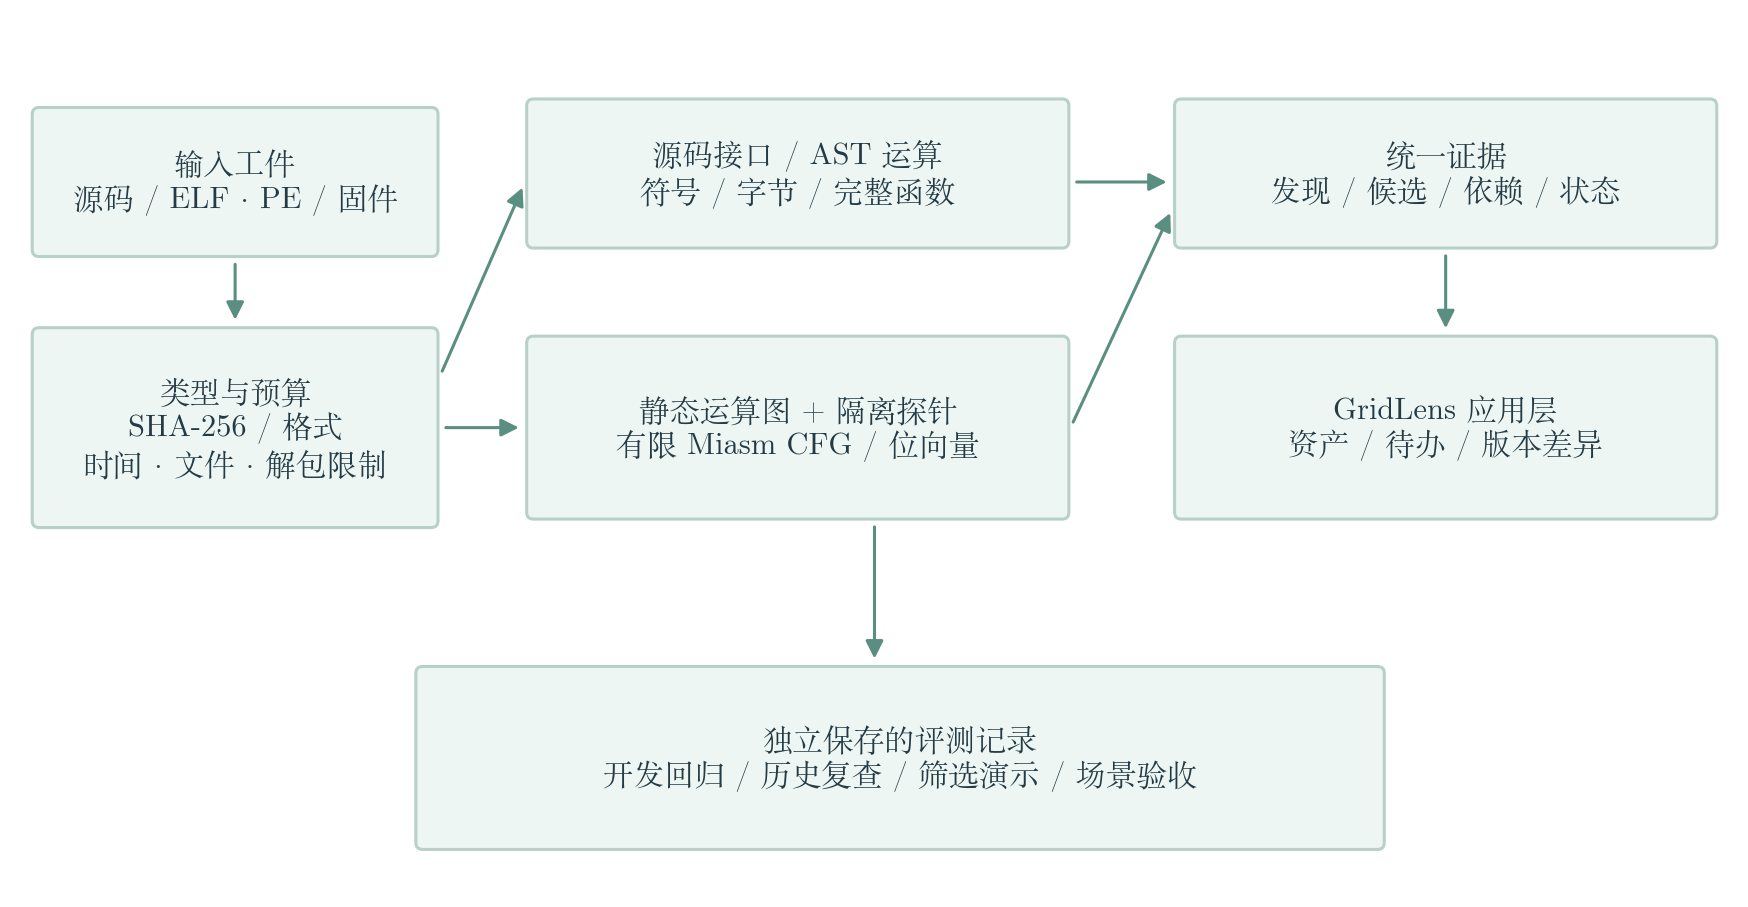
\includegraphics[width=\linewidth]{03-system-architecture.png}
  \caption{当前 QCS 检测引擎、证据模型与 GridLens 应用层。各分析通道按对象与预算适用。}
  \label{fig:qcs-principle-flow}
\end{figure}
% 配图注释（P03）：放一张横向系统架构示意图，区分输入、识别引擎、统一证据和应用层。
%   保留“候选/未知/状态”分支；不要把所有通道画成必定成功的线性流程。

\subsection{源码词法掩盖与接口角色判定}
\label{subsec:source-principle}

源码检测首先解码文本，再对注释和字符串进行词法处理。
当前实现采用严格 UTF-8 解码，失败后尝试严格 CP1252；
它不执行任意编码识别。
若把正则表达式直接应用于原始文件，
注释中的调用示例、字符串中的接口名称与真实调用可能具有相同外观。
因此，工具维护两个等长视图：
代码视图遮盖注释和字面量，
参数视图遮盖注释而保留字面量。
遮盖字符替换为空格，同时保留原始换行和字符位置。
由此可以在去除干扰后，仍将候选定位回原文件的行号。
对于多字节文本，字符位置不应直接等同于二进制字节偏移。

词法器处理行注释、块注释、转义引号、行续接和 C++ 原始字符串，
使 URL 内的双斜线不会错误截断字符串。
工具在代码视图中寻找已审核的精确接口名称，
结合括号与附近的语法形式，将候选分为调用、定义、声明、
宏定义以及名称或类型引用。
明确调用形成静态接口引用；已知算法接口的定义先形成命名依据，
只有源码摘要与已审核参考记录相符时，才形成固定源码实现证据。
另一条源码实现路径由后述语法树运算图及其见证约束支持。
声明、宏文本和普通名称仅形成线索。
例如，注释中的 \nolinkurl{mbedtls_aes_crypt_ecb(...)}
与真实调用使用同一接口名称，但不会获得相同证据角色。

直接选择参数用于补充通用接口的身份。
工具在保留字面量的视图中读取当前表达式的实参，
例如 \nolinkurl{EVP_MD_fetch} 的 \texttt{"SHA256"} 参数，
\nolinkurl{EVP_PKEY_CTX_new_id} 的 \nolinkurl{EVP_PKEY_RSA} 参数，
以及 Mbed TLS 的算法枚举或 \texttt{is224} 参数。
只有直接可见且符合审核规则的参数才参与算法细分。
设接口为 $f$、角色为 $r$、直接选择参数为 $s$，
其身份判定可写为
\begin{equation}
  A=\operatorname{Map}(f,r,s),
  \qquad A\in\mathcal{A}\cup\{\bot\},
  \label{eq:source-identity-map}
\end{equation}
其中 $\mathcal{A}$ 为可记录的算法集合，$\bot$ 表示身份未确定。
同一接口可能具有多算法含义；映射不要求每次返回一个单独算法。

这一接口路径属于词法与局部上下文分析，本身不构建抽象语法树。
独立的源码运算路径使用 Tree-sitter 及有限内部调用关联，
但整体仍没有完整展开预处理器、跟踪任意函数指针或进行全程序数据流分析。
未激活的条件编译分支仍可能被视为源码文本，
变量间接携带的选择器也可能无法恢复。
这些限制随报告说明，避免把源码引用解释成当前构建一定包含或运行的功能。
补充文本扫描得到的关键词和宽泛接口命中仅作为弱线索保存。

\subsection{程序格式解析与符号证据}
\label{subsec:symbol-principle}

结构化符号分析按照程序文件格式读取命名记录，
减少普通字符串、调试文本或文档内容对接口判定的干扰。
ELF 路径同时读取 \nolinkurl{.symtab} 和 \nolinkurl{.dynsym}，
保留符号表来源、地址、位宽和字节序。
符号所属节为 \nolinkurl{SHN_UNDEF} 时记为外部引用；
其余相应定义记为对象内部的命名证据。
来自两个表的同一符号去重后仍保存来源集合，
不会因为在两张表中出现而被计算为两个独立算法。

PE 路径通过命名导入和延迟导入记录接口及 DLL 来源。
只有序号的导入无法直接恢复算法名称，需保持未解析；
当前路径也不等价于全面识别静态链接 PE 内部的密码函数。
ELF 的 \nolinkurl{DT_NEEDED} 则单独形成库依赖。
依赖 \nolinkurl{libcrypto} 只能说明外部库关系，
不能展开为 AES、RSA、ECDSA 等全部算法均存在。

算法映射采用经审核的专用接口集合。
通用大整数、椭圆曲线点运算或通用 EVP 入口，
只支持其共享类别线索。
这使符号通道可以跨处理器读取标准格式，
但具体算法覆盖仍依赖接口命名与符号是否保留。
删除符号后未命中此通道，并不构成算法不存在的证据。

\subsection{字节规则、架构约束与共享特征}
\label{subsec:yara-principle}

YARA 通道对字节序列进行常量、表与机器码模式匹配\cite{yara-docs}。
设文件为 $B$，规则 $R$ 含模式 $p_1,\ldots,p_m$ 和布尔条件 $C_R$，
则原始命中为
\begin{equation}
  \operatorname{Hit}(R,B)
  =C_R\bigl(\operatorname{Match}(p_1,B),\ldots,
             \operatorname{Match}(p_m,B)\bigr).
  \label{eq:yara-raw-hit}
\end{equation}
该式只判断模式组合满足条件，未验证完整的密码运算语义。
整文件条件还可能把不同函数或数据区的模式合并为一次命中。
因此，本工具将原始规则与经过审核的算法含义映射分开管理。
映射记录证据类型、确定身份或候选集合、架构约束、
判别项和解释理由。

某条规则匹配到共享常量时，其候选集合可以表示为
\begin{equation}
  \Gamma(R)=\{a_1,\ldots,a_k\},\qquad k>1.
\end{equation}
共享 SHA-2/BLAKE2 IV、DES 基础表、ChaCha/Salsa 常量
以及 Keccak 置换特征均按这一原则处理。
对于含共享 IV 的 MD5/SHA-1 规则，还检查实际命中是否包含专用判别项。
缺少该项时保留候选，不直接沿用规则名称给出算法身份。
若规则未进入审核映射，记录未映射错误及原始线索，
并将扫描标为不完整。

架构约束在字节命中后再次检查。
x86-64 指令规则只有在程序架构已被结构化解析确认为 x86-64 时，
才按相应指令证据输出；
在其他或未知架构上，相同字节可能代表无关指令或数据，
因此抑制其算法身份。
常量规则具有较少的架构依赖，但仍受字节序、布局和表生成方式影响。
报告保存全部命中偏移、长度、十六进制字节、规则摘要及映射摘要，
便于回溯判定来源。

\subsection{整函数签名与地址变化处理}
\label{subsec:function-principle}

无符号程序缺少接口名称时，
本工具通过已知实现的整函数字节约束补充识别。
参考库选取固定版本的 Mbed TLS、TinyCrypt 和 micro-ecc，
从带符号构建中取得操作函数的边界与算法角色
\cite{mbedtls-source,micro-ecc-source,esp-idf-source}。
识别目标仍是特定参考构建中的已知代码，
而不是从任意大整数或点运算推断密码算法。

同一函数在不同链接布局下，调用地址、相对位移和常量地址可能改变。
直接比较所有字节会将这类变化误作不同实现；
任意放宽指令字节又会丢失计算行为的区分能力。
本工具读取参考可重定位对象中的真实重定位记录，
将对应地址字段转换为逐位掩码，
与链接后函数字节配对。
掩码保留操作码、寄存器、非地址立即数与函数长度。
AArch64 的链接松弛可能将 \texttt{ADRP+ADD} 改写为 \texttt{NOP+ADR}，
建库时按最终指令重新处理其地址字段。
因此，掩码来源是可审计的构建记录，而不是猜测哪些字节可以忽略。

设参考函数字节为 $F=(f_0,\ldots,f_{L-1})$，
掩码为 $M=(m_0,\ldots,m_{L-1})$，
候选目标位置为 $o$。
当掩码位为 1 时要求该位精确一致，
整函数约束为
\begin{equation}
  \operatorname{BodyMatch}(F,M,B,o)
  =\bigwedge_{i=0}^{L-1}
    \bigl(((B_{o+i}\oplus f_i)\land m_i)=0\bigr).
  \label{eq:whole-function-mask}
\end{equation}
候选范围必须完整落在可执行段内，并满足记录的长度与对齐约束；
工具不据此恢复目标程序的全部函数边界。
候选来自目标 ELF 的可执行 \nolinkurl{PT_LOAD} 段，
从而排除仅存放在非可执行数据段中的函数字节拷贝。
它仍不证明相应代码会在业务中执行。

为减少整段逐位置比较，工具选择长度不超过 64 字节、
有效约束位最多的短窗口，用 YARA 先定位候选。
YARA 的十六进制通配只能表达较粗的位约束，
短窗口结果随后按式~\eqref{eq:whole-function-mask} 对全部字节逐位复核。
短锚点独立命中不会产生算法发现，
最终结论取决于完整函数约束。
运行时无需目标函数名，也不依赖完整反汇编或学习模型。

\subsection{只读常量约束与散列角色组合}
\label{subsec:hash-disambiguation}

地址字段被遮盖后，还必须验证目标函数实际引用的数据。
否则，初始化指令形式相同但常量不同的散列变体，
可能满足相同代码掩码。
建库时记录 x86 RIP 相对寻址、AArch64 页相对加载所引用的只读常量；
运行时从目标函数的真实位移恢复地址并核对常量内容。
当前 ARM 参考函数内的常量池保持为精确字节约束。
文件中另放一张未被函数引用的 IV 或轮常量表，不满足这一条件。

若 $\mathcal{L}_F$ 为函数记录的常量约束集合，
完整函数匹配要求
\begin{equation}
  \operatorname{FunctionMatch}
  =\operatorname{BodyMatch}
   \land\bigwedge_{\ell\in\mathcal{L}_F}
       \operatorname{LiteralMatch}(B,o,\ell).
  \label{eq:function-literal-match}
\end{equation}
地址重定位容忍链接布局变化，
常量约束保留算法参数差异，二者共同决定识别范围。

对 SHA-256，还需要同一实现家族的互补函数角色。
设家族 $g$ 的必要角色为 $\mathcal{R}_g$，
已匹配角色集合为 $\mathcal{W}_g$，则
\begin{equation}
  \operatorname{FamilyComplete}(g)
  \iff \mathcal{R}_g\subseteq\mathcal{W}_g.
  \label{eq:family-role-completeness}
\end{equation}
TinyCrypt 使用初始化与最终输出角色，
Mbed TLS 使用初始化与压缩角色。
仅有共享压缩或不完整初始化证据时，输出仍为候选。
角色组合在同一对象与参考家族内核对，
不会将不同库的任意函数拼成新的完整实现。
RSA、ECDSA 和 ECDH 则要求匹配算法操作、签名或协商函数，
不使用通用大数、点乘函数替代这些角色。

当前数据库适用于小端 x86-64、AArch64 和 ARM 模式的链接 ELF。
编译器、版本、优化、配置宏、内联、LTO 与混淆变化均可改变整函数形式。
因此函数签名证据记为中等级别的已知实现证据，
并随之记录参考构建摘要、签名标识、匹配函数及数据库摘要。
未匹配到已知库不能解释为没有非对称算法。

\subsection{固件组件提取与来源可追溯性}
\label{subsec:firmware-principle}

固件镜像可能包含引导头、压缩文件系统与多个程序组件。
当前优先使用经审核的原生 SquashFS、gzip 与受限 ESP 适配器；
SquashFS 通过 \texttt{unsquashfs} 在临时目录中提取文件。
锁定版本的 Binwalk 2 属于可选历史回退，在本文最终环境中不可用，
不能将其写成这一环境已经成功运行的必要依赖。
解包后逐文件检查类型，再调用已有源码、程序或固件入口。
工具不执行下载的目标程序，
但提取过程会运行外部解包器；临时目录和资源限制不等价于完整安全沙箱。

固件内证据通过镜像摘要、组件摘要、文件系统内路径与解包链关联。
普通文件摘要为内容 SHA-256；
目录摘要则由排序路径和组件摘要组合，二者含义分别记录。
嵌套镜像使用 \texttt{!/} 连接逻辑路径，
报告中的稳定组件标识由外层镜像摘要和逻辑路径构成，
避免把已删除的临时绝对路径作为资产位置。
只有能明确对应时才保存文件系统镜像偏移；
多个文件系统无法对应时保持空值。
压缩文件中的解压后偏移也不能直接当作外层固件字节偏移。

组件扫描不跟随符号链接，
目录遍历和嵌套提取共享文件数、总字节、递归深度与时间预算。
达到限制时保留已经取得的证据，并明确未处理部分。
原生适配器覆盖之外的容器、加密区域和不可解析镜像，
记录为不支持或失败，而不返回虚假的完整阴性报告。

\subsection{证据归一化、资产汇总与完成状态}
\label{subsec:report-principle}

每条证据保存算法、类别、引擎、标识、行号或偏移、
置信等级及理由，并附带通道特有信息。
本工具将能够支持明确算法身份的静态证据放入发现集合，
将共享候选、编码特征与宽泛名称放入线索集合，
库依赖和错误独立记录。
这种组织保留证据的原始含义，
不会通过多条弱线索投票把共享结构自动升级为确定身份。

设算法 $a$ 的发现证据集合为 $E_a$，
资产汇总保留全部 $E_a$，并按
$\mathrm{low}<\mathrm{medium}<\mathrm{high}$ 的序关系取最高等级：
\begin{equation}
  c(a)=\max_{e\in E_a}c(e).
\end{equation}
这一等级表示规则依据的相对强弱，
没有通过校准转换为正确概率。
多条规则命中同一算法时，仍只形成一个规范算法资产，
但具体证据及组件归属继续保留。
固件顶层汇总递归收集组件发现，因此顶层局部发现列表为空
不表示整幅镜像没有算法资产。

扫描状态区分流程是否完成与算法是否识别正确，见表~\ref{tab:qcs-status}。
已取得有效结果但存在错误、受限通道或未支持组件时，通常归为部分完成；
没有有效通道且发生错误时归为失败。
有意关闭或不适用的通道单独标为停用，不必然令其他成功通道失败。
缺失依赖、规则编译失败和超时均保留错误信息，
不会被静默转换为空发现。

\begin{table}[htbp]
  \centering\small
  \caption{扫描状态的含义及命令行退出码}
  \label{tab:qcs-status}
  \begin{tabularx}{\linewidth}{l c X}
    \toprule
    状态 & 退出码 & 解释\\
    \midrule
    \texttt{completed} & 0 & 支持范围内的步骤完成；不代表算法不存在或识别全部正确。\\
    \texttt{partial} & 2 & 已保留部分结果，但存在限制、失败通道或未支持组件。\\
    \texttt{unsupported} & 3 & 当前无法按指定方式分析该对象。\\
    \texttt{failed} & 4 & 输入或必要处理失败，不能获得相应完整结果。\\
    \bottomrule
  \end{tabularx}
\end{table}

\subsection{资源控制与双口径评测的联系}

扫描器默认使用 60 秒时间预算、10000 个文件、4 层固件递归、
1 GiB 总字节与 256 MiB 单文件限制。
外部提取进程在超过预算时终止其进程组，
组件分析也继续沿用同一预算对象。
这些机制减少失控遍历和过量提取，但依赖周期性监测，
不能宣称为严格的实时内核限额。

报告中的证据角色直接决定评测口径。
源码明确调用与二进制导入进入接口引用集合；
与固定参考摘要相符的源码实现、带标准依赖见证的源码运算图、
已定义符号、审核后的常量/指令和整函数签名进入实现包含集合。
单纯源码命名定义不进入该集合。
共享候选不进入任何确定预测集合。
两种集合分别与预先标注的真值比较，
因此工具可以区分“引用了外部接口”和“对象内含实现”的检测效果。
第三章给出样本构建、真值审核、执行命令和指标计算方案，
第四章按这些约定给出已经完成的实验结果和未完成事项。

\section{运算语义、有限控制流与原语摘要}
\subsection{从代码特征到带数据依赖的运算见证}
后续版本增加源码语法树、指令解码、局部表达式与静态调用关系，
使识别不完全依赖函数名或单个字节序列。
例如，SHA-256 的轮计算需要关联 $\mathrm{Ch}$、$\mathrm{Maj}$、
大/小 $\Sigma$、消息调度、实际使用的轮常量和 SHA-256 IV；
共享 SHA-224 压缩结构不能单独确认 SHA-256。
SM4 需要关联表查找、特定线性变换、轮密钥与反馈，
公钥识别需要满足已实现的模运算或曲线协议关系。
源码侧有限关联局部头文件、数组初始化和内部调用，
但没有替代编译器完整的预处理、类型系统与全程序分析。

对加法、异或和旋转作正规化时保留输入身份与字宽。
例如同一 32 位值的左右移位可合并为旋转，
结合律加法可以展平，低 32 位截断只对相容的运算下推。
若把不同分支或无关输入上的旋转混合统计，可能得到假的轮结构；
因此算法见证由同一有界依赖图支持，而非仅由运算出现次数支持。

\subsection{Miasm 的进程隔离与有限 CFG}
Miasm 将机器指令提升为中间表示，再执行符号状态传播\cite{miasm}。
自写控制器验证请求、选择固定外部解释器、限制资源，并以 JSON 交换结果。
原生指令与指令内部 IR 块都进入有界工作队列。
相对分支先正规化为地址标签，寄存器别名和零扩展由提升语义处理。
当前有限直接 CFG 主要覆盖 x86-64、ARM、Thumb 与 AArch64；
MIPS 大小端可处理其已支持直线片段，延迟槽控制转移是显式边界。
调用、间接边及 Thumb IT 等未完整处理时保留部分状态，而不推断完整出口语义。

令状态映射 $S$ 为寄存器或可确认位置到表达式的映射，
两路径合并采用相同事实保留策略：
\begin{equation}
 (S_1\sqcup S_2)(x)=
 \begin{cases}
 S_1(x),&S_1(x)=S_2(x),\\
 \mathrm{unknown}_{x,w},&\text{否则}.
 \end{cases}
\end{equation}
其中 unknown 具有稳定身份和位宽 $w$。
循环中冲突值扩大为 unknown，以推动保守收敛；
该方法不证明全部路径可达性，也不是 SMT 驱动的完整路径求解。
内存写可能与既有事实别名，因而保守清除旧内存事实，
只保留可确认的最新精确地址写后读。
预算耗尽且未收敛时不输出临时表达式作为完整摘要。

\subsection{带位宽、输入身份与来源的摘要}
位向量加法写为
\begin{equation}
 z=\operatorname{add}_w(x,y)=(x+y)\bmod 2^w.
\end{equation}
同一宽乘在 32 位和 64 位语义下具有不同截断和高位输出，不能丢弃位宽。
摘要包含表达式标识、操作数引用、输入身份、位宽、地址范围、代码摘要及覆盖说明。
进位、借位和宽乘可记录为原语，但其字段为
\nolinkurl{primitive_only=true}、\nolinkurl{algorithm_eligible=false}。
这些记录不自动等价于 Montgomery 约减、模幂、模逆或曲线协议。
当前生产桥接主要消费合并后的寄存器出口表达式，
独立 API 可返回的内存结果尚未完整接入算法消费。

后端每次限制 256 条原生指令、512 个 IR 块、1024 个 IR 步和 32768 个表达式节点，
地址空间上限 512 MiB、输出上限 512 KiB；
摘要还限制至多 64 个不同运算公式、4096 个公式节点。
这些上限是工程预算，不意味着分析范围恰好覆盖一个完整函数。

\subsection{原语与算法的桥接边界}
已有识别器可以从满足依赖条件的 32 位表达式恢复 ChaCha 四分之一轮：
\begin{align}
 a&\leftarrow a+b,&d&\leftarrow\operatorname{ROTL}_{32}(d\oplus a,16),\\
 c&\leftarrow c+d,&b&\leftarrow\operatorname{ROTL}_{32}(b\oplus c,12),\\
 a&\leftarrow a+b,&d&\leftarrow\operatorname{ROTL}_{32}(d\oplus a,8),\\
 c&\leftarrow c+d,&b&\leftarrow\operatorname{ROTL}_{32}(b\oplus c,7).
\end{align}
四个输入的身份和更新次序是依据的一部分；
单独出现 16、12、8、7 四个常量不构成等价证据。
这一桥接通过针对性正反例，不代表后端已在未知生产实现中新增检出。
RSA 与曲线算法仍需 ABI、输出缓冲区、调用副作用和完整协议方程的进一步约束。
二进制通常丢失源变量名、类型和宏信息，提升 IR 或生成伪代码不等于恢复原始源码。

\section{从识别证据到迁移待办的原理}
GridLens 将资产按“文件、算法、证据范围”合并，保留核心证据与原始报告入口。
业务模块来自显式场景清单，风险类别来自可审查规则：
MD5/SHA-1 等进入遗留用途复核，传统公钥接口进入量子迁移关注，
其他对称和摘要资产进入模式、密钥或用途复核。
动态提供者调用而算法参数未知时单列覆盖待确认，不计成具体算法资产。
迁移任务引用相应资产或文件，人工状态独立存储，不能反向修改算法发现。

% 配图 P04：真实源码证据弹窗，需看清输入哈希、行号、MD5 调用和原始报告入口。
\begin{figure}[htbp]\centering
  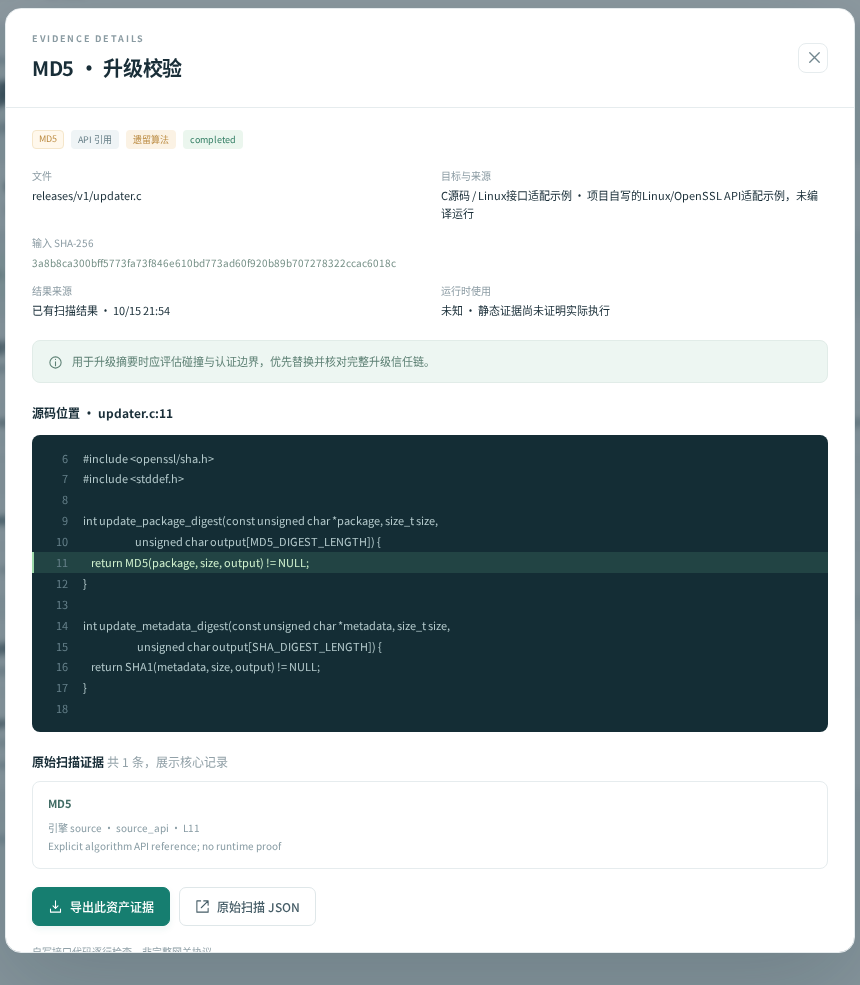
\includegraphics[width=.82\linewidth,height=.72\textheight,keepaspectratio]{04-source-evidence.png}
  \caption{GridLens 展示真实源码扫描证据。高亮行、输入哈希及原始报告入口构成可审查链。}
  \label{fig:source-evidence}
\end{figure}
% 配图注释（P04）：放界面局部截图而非流程图：保留 MD5 调用高亮、文件路径、SHA-256 与证据类型。
%   截图只裁去无关页边，不更改扫描数字；避免缩到无法阅读源码。

\chapter{系统设计与实验方案}\section{研究问题与实验分层}
实验以竞赛作品展示为主，重点回答：固定软件工件上的识别结果能否复现，
证据是否可追溯，以及发布前体检和整改对比是否形成可操作的演示闭环。
另保留完整开发与历史不同作者结果，供解释识别范围和后续改进使用。

\begin{table}[htbp]\centering\small
\caption{实验层次、输入和结论边界}\label{tab:experiment-layers}
\begin{tabularx}{\linewidth}{p{2.2cm}p{3.4cm}X}\toprule
层次 & 输入与固定条件 & 要回答的问题\\\midrule
十三算法复扫 & 开发总体的全部源码及双架构程序，共 1071 份 & 第四章主实验：十三算法的范围内漏报及分载体差异。\\
混合演示复扫 & 五算法、两架构、241 份源码/程序；来源分列 & 保留旧紧凑演示的可复现结果，不代替十三算法主实验。\\
网关应用验收 & 两版源码、四份 SDK、四个视图 & 证据、迁移待办、差异、离线网页和现场调用是否连通。\\
开发回归 & 2344 文件、六份开发清单，按内容去重 & 附录保留已知家族覆盖和原有规则回归结果。\\
历史验证复查 & 2855 / 232 / 252 文件，沿用原锁及源码边界 & 附录保留既有不同实现覆盖；不是新的盲测。\\\bottomrule
\end{tabularx}\end{table}

历史结果来自已经完成并留存的实验，本轮重新核算其 JSON；
已完成的 241 份混合演示及五类固件实验继续保留；
本轮另对按载体和架构全取的 1071 份开发输入实际新扫。
没有重新训练模型、修改识别器或重跑完整历史样本库。
图表生成脚本从同一份证据摘要生成表格，原报告路径与哈希保存在附录及
\nolinkurl{data/evidence.json} 中。

\section{系统架构与工程环境}
\subsection{检测引擎与应用层分工}
主工程位于 \nolinkurl{ustc_tool_middle/}，Python 包位于 \nolinkurl{src/qcs/}。
统一入口提供 \texttt{doctor}、\texttt{scan}、\texttt{evaluate}；
固定多清单实验另有开发与历史复查运行器。
GridLens 位于 \nolinkurl{examples/gridlens/}，只消费真实报告和显式场景标注，
不为展示重新创造一套算法识别规则。

\begin{table}[htbp]\centering\small
\caption{实现模块与可审查职责}\label{tab:module-layout}
\begin{tabularx}{\linewidth}{p{5.2cm}X}\toprule
模块 & 主要职责\\\midrule
\nolinkurl{scanner.py}, \nolinkurl{model.py} & 对象分派、预算、状态、证据与双口径预测。\\
\nolinkurl{source.py}, \nolinkurl{api_rules.py}, \nolinkurl{source_reference.py} & 词法角色、参数映射、已审核源码引用及身份核验。\\
\nolinkurl{symbols.py}, \nolinkurl{yara_engine.py}, \nolinkurl{function_signatures.py} & 符号、规则、可执行段内完整函数及常量核验。\\
\nolinkurl{operations.py}, \nolinkurl{guomi/}, \nolinkurl{semantic_probes.py} & 源码/二进制运算见证、国密和隔离指令探针。\\
\nolinkurl{miasm_backend.py}, \nolinkurl{miasm_worker.py}, \nolinkurl{miasm_summary.py}, \nolinkurl{miasm_scan.py} & 外部环境控制、有限 CFG、位向量摘要和现有算法桥接。\\
\nolinkurl{firmware.py}, \nolinkurl{firmware_native.py} & 固件结构校验、受限提取、组件递归和来源链。\\
GridLens 的 \nolinkurl{assessment.py}, \nolinkurl{server.py}, \nolinkurl{app.js} & 资产组织、规则待办、本机扫描服务与离线网页。\\\bottomrule
\end{tabularx}\end{table}

\subsection{解释器、依赖与资源控制}
主引擎使用 Python 3.12.3 隔离环境。已保存 doctor 记录确认
YARA 4.5.4、pyelftools 0.32、pefile 2024.8.26、Capstone 5.0.6、
Tree-sitter 0.25.2、Unicorn 2.1.4 等运行依赖可用。
国密解析器与规则、源码参考库、函数库均带摘要；普通函数签名库为 1028 条，
国密参考与开发签名库分别为 152 和 211 条。
这些是数据库记录数，不是算法种类数、独立实现数或正确检出数。
Miasm 固定提交为 \nolinkurl{3671fc24d6e625c2d75f3311724eb6b0c97664f8}，
运行在独立环境，保留 GPL-2.0-only 许可\cite{miasm}。
Binwalk 在该份最终 doctor 中缺失或不支持，但原生适配器和 SquashFS 工具可用。

本机修订时可见环境为 Fedora CoreOS 42、x86-64、Intel Xeon Silver 4410Y，
可见逻辑 CPU 为 48 个；这份机器信息是本轮采集，未冒充历史每次运行的资源监测。
历史批次并发条件按原记录保留：三批历史复查使用 32 进程，
旧筛选演示复扫两批各 16 进程并行；本轮混合演示使用 16 进程单批复扫。

默认每对象预算为 60 秒、10000 文件、4 层固件递归、1 GiB 总字节和 256 MiB 单文件。
目录与镜像组件共享预算；固定集合评测则逐文件独立预算。
Miasm 阶段最多两个候选、合计 3 秒、单次不超过 1.5 秒，消耗原总时限的剩余部分。
GridLens 的单文件外部进程上限为 85 秒，演示配置关闭 Miasm，
因此其六文件速度不能与默认开启后端的全量实验直接比较。

\section{样本、真值与冻结方案}
\subsection{真值单位和标注范围}
主实验的单位是\textbf{文件--算法标签}。
每行含输入路径、内容 SHA-256、项目、实现家族、架构、编译参数、符号状态、
真实存在集合 $T_i$ 及已标注算法范围 $K_i$。
未在 $K_i$ 中的算法不当作阴性；同一文件可以同时存在多个正标签。
源码、构建模块及编译宏共同决定实现真值，函数名本身不作为独立语义正确性证明。

原始资料库包含 12870 份不同内容、12900 个物理文件，
其中有头文件、建库参考、许可配套和排除来源。
这些存量数不进入实验分母。
开发清单按内容合并时核对共同标注范围，避免把同字节的不同构建名称重复计数。
相同作者的多个优化级别仍属于同一实现家族，不作为独立作者样本。

\subsection{源码上下文与程序构建边界}
源码运算识别可能使用局部头文件和明确调用关系，
所以比较前固定源文件以及允许的上下文路径。
历史复查沿用原隔离源码边界；若当前工作树旁出现开发文件，不能扩大为可见上下文。
缺少局部依赖的源码片段，其实现级漏报与 API 调用级检出并非同一问题。
程序构建保存优化参数与架构，对剥离符号、共享库或仅模块构建分别注明；
未编译成功的尝试不伪装成完成的扫描输入。

\subsection{冻结及本轮证据核验}
历史复查使用的最终检测包摘要为
\nolinkurl{16dc3c38dd4f8d1e9ef4da1ff3307a8b438ae34381361386992e93f2c09af2c3}。
记录冻结了代码、样本与外部环境，并在运行后再次核验。
开发汇总在修正 MIPS 输出寄存器接口后重扫了受影响的 560 个文件，
另 1784 份结果按未受影响的代码行为复用并保留原始报告哈希；
不能称最终版本再次完整新扫了全部 2344 文件。
三批历史复查则全部新扫，未根据本轮历史预测继续调规则。
这些集合已经在之前开发周期中被观察，因此本文称其为历史验证复查。

\section{三类载体的实验实施方案}
\subsection{源码实验}
先计算摘要并解码，分别构造代码与参数视图，
识别专用接口、直接算法选择参数、调用/定义/声明角色；
在可用范围内进一步检查语法树运算、查表来源、指针关联及有限内部调用。
设置注释、声明、普通字符串、动态变量、共享常量和通用大数阴性对照。
验收既检查能否找到阳性，也检查不充分线索是否保持未知。

\subsection{ELF/PE 程序实验}
校验格式与架构后，依次运行符号、字节、函数签名、国密运算、
静态语义及隔离探针，再在剩余预算中尝试 Miasm。
参考函数须在可执行段匹配，重定位字段需掩盖，使用只读常量核对区分共享轮函数。
PE 的已验证路径主要依赖结构化导入与相应字节规则，
不把 ELF 整函数签名或各 ISA 的部分语义能力转述为 PE 全面覆盖。
遇到通道失败保留其他结果，并记录部分完成。

\subsection{固件实验}
对受支持的 SquashFS、gzip 和 ESP 容器先检查长度、头部、校验及段范围，
按限制提取组件并记录镜像摘要、相对路径、偏移和提取链。
可识别组件进入同一引擎；未支持的区域保持说明，不返回完整阴性结论。
当前三批主结果以源码和可执行文件为主，未单列真实终端固件总体准确率；
固件结论由工程适配与相应回归记录支持，不能拿主表替代固件效果统计。

\section{评测指标与错误处理}
设第 $i$ 个文件在口径 $s$ 上的预测为 $P_i^{(s)}$，
只在 $K_i$ 范围内比较。接口引用与实现包含分别计算，不相互充当命中。
主结果采用实现包含口径，计数为
\begin{align}
TP&=\sum_i |P_i\cap T_i\cap K_i|,&
FN&=\sum_i |T_i\setminus P_i|,\\
FP&=\sum_i |(P_i\setminus T_i)\cap K_i|,&
TN&=\sum_i |K_i\setminus(T_i\cup P_i)|.
\end{align}
由此定义
\begin{align}
\operatorname{Recall}&=\frac{TP}{TP+FN},&
\operatorname{FNR}&=\frac{FN}{TP+FN},\\
\operatorname{Precision}&=\frac{TP}{TP+FP},&
\operatorname{Accuracy}&=\frac{TP+TN}{TP+FP+FN+TN}.
\end{align}
误报率为 $FP/(FP+TN)$，与 $1-\operatorname{Precision}$ 不同。
分母为零时标为不适用。总体准确率可能被大量阴性标签抬高，
故必须同时报告召回率、漏报和绝对计数。
同一文件的多个变体相关，不给出假设标签独立的置信区间来夸大样本量。

扫描完成度也不等于正确率。
\texttt{partial}、失败和预算耗尽不从固定分母删除，已取得预测仍保留；
否则会把难样本通过运行状态过滤掉。
报告按算法、载体和架构分组，定位错误而不修改已锁定真值。

\section{语义后端对照方案}
Miasm 首先接受 ISA 夹具与数值真值测试，再进行开发对照，最后冻结后做三批历史复查。
对照核对逐文件预测、候选状态、原语数及阶段耗时。
接入前后扫描器并非只改变一个开关的严格单因素消融，旧探针存在时间波动，
因此明确区分后端直接产生的标签与其他引擎新增标签。
若后端仅返回大数原语，不能计作 RSA、ECDH、ECDSA 或 SM2 检出。
本轮没有完成每个通道逐一关闭的全量消融，也没有其他工具同条件排名实验。

\section{十三算法与分载体复扫方案}
\label{sec:algorithm-suite-method}
\subsection{算法范围与业务解释}
本轮算法范围与第二章逐项对应：分组密码 AES、DES、SM4；
流密码 RC4、ChaCha20；公钥机制 RSA、ECDSA、ECDH、SM2；
摘要 MD5、SHA-1、SHA-256、SM3。
DES、RC4、MD5、SHA-1 用作遗留资产识别对象；
RSA 及曲线机制支持解释身份认证、升级签名和密钥协商的量子迁移关注，
不要求五类最小业务样例各自包含所有算法。
Shor、Grover 是风险解释的理论依据，当前工具没有执行量子算法，
不将其列入静态密码实现识别的十三种标签。

\subsection{输入全取、冻结与目标}
在已保存的 2344 份开发输入中，纳入所有源码，以及所有 x86-64、ARM64 程序。
这一架构范围沿用原展示定位；不再按算法命中、项目、优化等级、符号状态或阴性配额筛选。
1071 份不同内容输入包括 154 份源码、527 份 x86-64 程序和 390 份 ARM64 程序；
其余 1273 份为其他机器架构，仍保留在完整开发报告中。
原开发结果已经被观察过，因此这是已知家族回归；全取政策不使它成为独立验证。

原样保留每个输入的 \texttt{truth} 和 \texttt{known\_algorithms}；
范围外或未完整标注的算法不改标为阴性。
源码复制完整的配套上下文，所有扫描入口与上下文文件在复扫前锁定，
同时锁定总体清单、纳入清单、检测器与运行时。
使用默认 Miasm 开启配置、逐文件 60 秒预算与 16 个进程，
全部新扫报告逐文件保存；部分、失败和漏报均留在固定分母中。
扫描前后的哈希必须一致，不根据新结果重选样本。

每算法的验收目标为 \(\operatorname{FNR}_a\leq10\%\)，
由 \(FN_a/(TP_a+FN_a)\) 计算，并显示正标签数、TP/FP/FN 和目标状态。
10.00\% 属于等于上限，不能写成严格低于 10\%。
精确率 \(TP/(TP+FP)\) 描述误报，不用于替代漏报目标，
保留实测值，不为获得特定外观添加错误标签。
另将源码、x86-64、ARM64 的漏报分列；混合范围达标不推出单一载体均达标。

\section{筛选演示集与网关场景方案}
\subsection{五算法混合演示清单}
五算法演示范围限定为 AES、SM4、SM3、MD5、SHA-1，以及 x86-64 / ARM64 ELF64。
二进制从旧五算法精简集取样；旧集已按项目、家族、架构和原真值分组，
每组选择已观察表现较好的编译变体，因此带有表现选择偏差。
本轮保留其中全部阳性输入，包括已有漏报；阴性按来源和架构各取 SHA-256 排序前 10 份。
开发源码每算法选择 5 份已观察成功样例，优先不同真实上游项目，
不足部分再按项目、家族和 SHA-256 排序补齐，另加 5 份范围内阴性。
同项目多个文件不称为不同作者，源码上下文也不当作新增扫描根。

清单共 241 份，开发二进制、历史二进制和开发源码分为三个来源字段，
文件内容按 SHA-256 去重。既有完整真值和标注范围继续保留，
本轮计数只在原范围与五算法范围的交集中进行；其他算法不改标为不存在。
原始样本库和验证集均保留，本轮只建立单独的演示输入副本。
所有输入、源码上下文、清单和检测器在扫描前锁定，复扫后不根据新成绩再次挑选。
这是一项混合演示实验，不具备独立验证所要求的开发/测试隔离。

\subsection{虚拟网关双版本}
四模块固定为遥测通信、升级校验、身份认证、第三方插件。
两个版本各有三份 C 适配源码，另有一份共享动态提供者源码和两架构各两份共享 ELF，
合计 11 个路径输入；身份源码在两版相同，不称为 11 个独立算法实现。
每视图使用 4 份源码与目标架构的 2 份 ELF。
源码适配代码未编译运行；SDK 由已有开发样本复制并核验哈希，业务归属为人工场景标注。

v1 使用 MD5/SHA-1 升级摘要和 AES-128-CBC 遥测适配；
v2 改为 SHA-256/SM3 和 AES-256-GCM。
两版仍保留 ECDH、RSA、ECDSA 接口，以说明摘要治理和公钥量子迁移是不同任务。
动态提供者使用运行时名称，不预设具体算法。

% 配图 P02：双版本真实源码片段的左右对照，不使用抽象迁移流程代替实际代码。
\begin{figure}[htbp]\centering
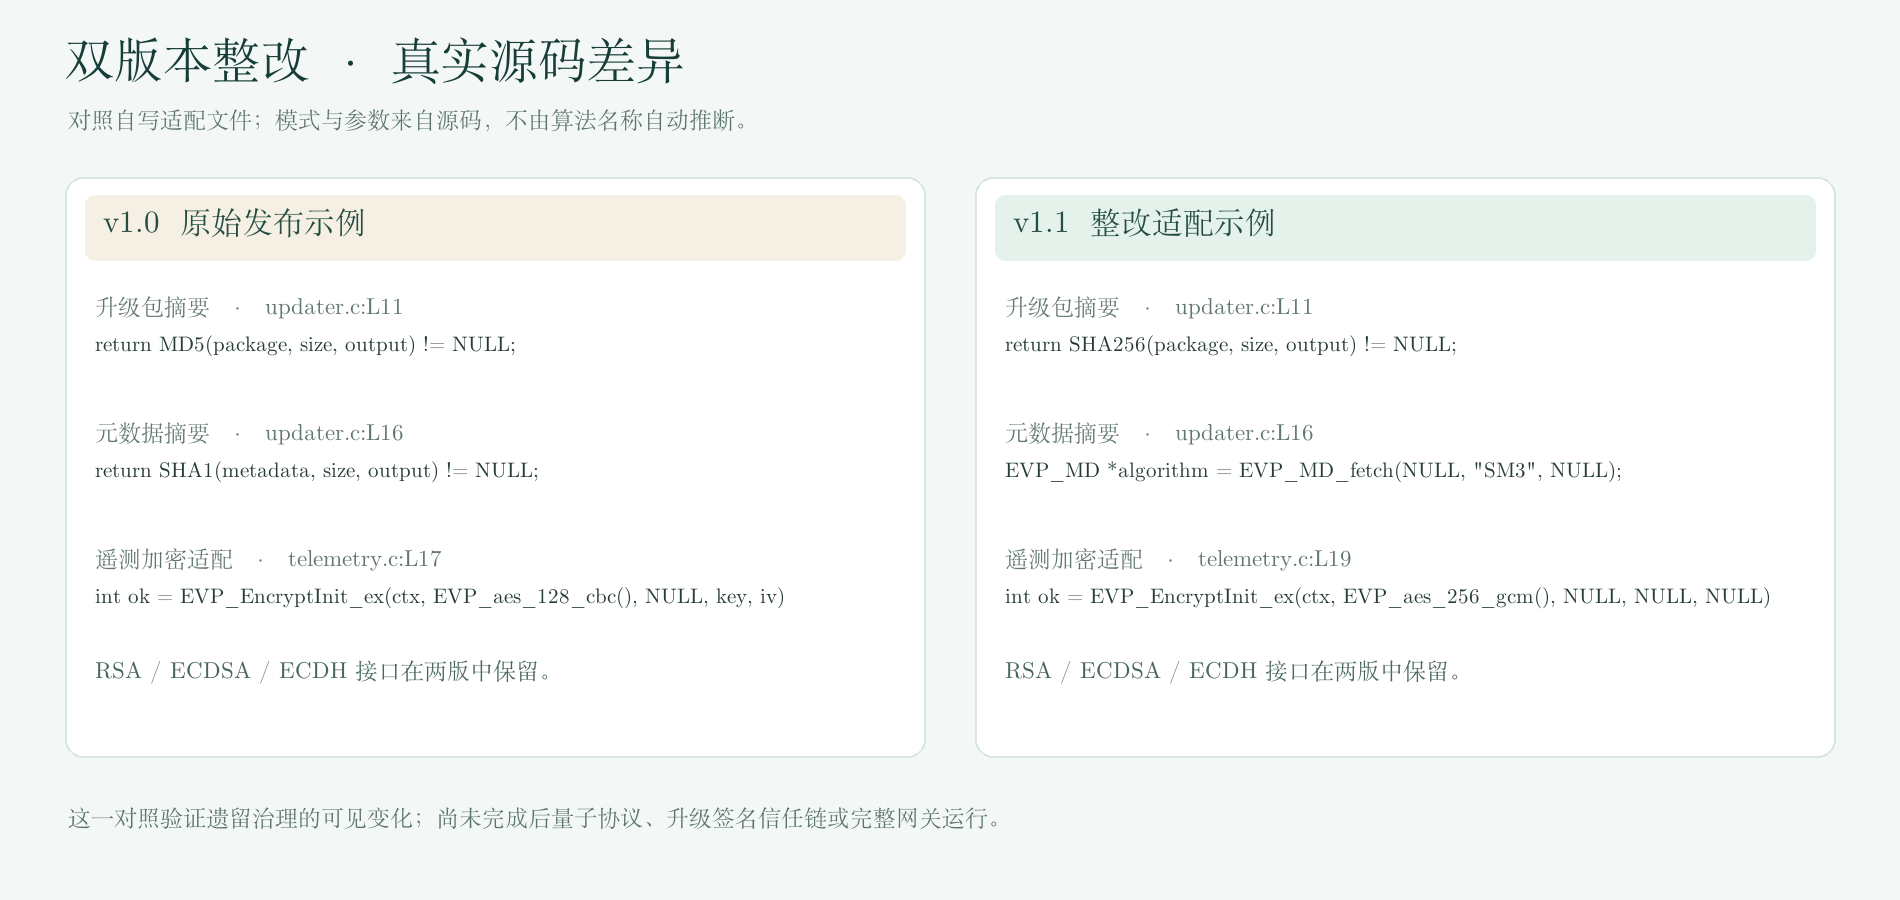
\includegraphics[width=\linewidth]{02-release-diff.png}
\caption{原始发布与整改适配的源码片段对照。两版公钥接口仍保留，摘要更换不等于完成后量子迁移。}
\label{fig:release-diff}
\end{figure}
% 配图注释（P02）：放左右两列代码样张，分别显示 MD5/SHA-1 与 SHA-256/SM3、
% AES-CBC 与 AES-GCM 的实际接口行；保留行号和文件名，并注明这是自写适配代码。

\subsection{交互与现场验收}
网页无外部 CDN，已有扫描数据作为本地脚本加载，适配 Windows 直接文件打开。
Linux 标准库服务只接受场景中的固定版本和架构，一次运行一个任务，
逐文件调用 QCS 并保存原始 JSON；失败不覆盖已有有效报告。
验收覆盖五页导航、四种视口、证据筛选与高亮、人工状态、导入导出、导览、回放与 PDF。
真实现场任务与离线回放分开标记，人工“已纳入计划”不修改扫描结论。

\section{五类电力终端的固件软件验证方案}
\label{sec:terminal-plan}
为检验从固件交付到密码证据的实际路径，另建五类终端软件场景：
智能电能表、用电信息采集集中器、配电自动化终端 FTU、继电保护装置 IED 和电力边缘网关。
业务程序分别执行电量累加、多表汇聚、事件序号检查、过流记录和主题路由，
不是把同一程序改五个名称。
每类具有独立源码、固定输入、预期业务输出和清单，在扫描前锁定。
密码源码来自已归属的教学实现与 OpenSSL，不把复用源码计为独立算法家族。

每类以 Zig 0.13.0 编译 x86-64 和 ARM64 的 Linux ELF 业务程序及共享库，
去掉静态符号，放入最小文件系统，再用 mksquashfs 生成 gzip 压缩的 SquashFS 镜像。
镜像与交付说明组成 ZIP，形成 10 份不同内容的交付包。
源码独立保留在构建目录，固件内只放程序、库、配置、固定业务数据及许可说明。
镜像没有内核、引导程序和完整系统运行库，不作为可启动设备固件。

验证先读取交付清单并核对 ZIP 与镜像 SHA-256，识别 SquashFS 后使用 unsquashfs 实际解包，
逐文件核对路径和内容哈希；再将镜像交给现有 QCS 固件入口，
由它再次解包并递归分析 ELF 与文本，保留固件哈希、组件路径、文件哈希及证据。
内容哈希校验不等于厂商签名认证，本实验没有提供真实厂商证书。
不要求从二进制恢复源码：固件通常只含机器码、库和配置，直接进行二进制静态识别即可。

每镜像包含两个已声明 ELF。五算法范围 AES、SM4、SHA-256、SHA-1、MD5 的实现标签
由构建源码和链接清单确定；文本及许可文件只计入提取清单，不作为实现阴性标签。
使用每镜像 180 秒预算、3 个并行任务，Miasm 关闭，
扫描前后核对识别器、runtime 和清单摘要，没有据新结果重新选择输入。
另运行五类提取后的 x86-64 程序，检查业务断言和所用密码的已知答案；
ARM64 仅交叉编译与静态扫描，未声明其运行验证。
这一软件级流程实验独立于 241 份混合演示清单，指标不合并。

\section{复现操作与记录保存}
单对象入口如下，输出统一放入新的目录，避免覆盖历史记录。
\begin{lstlisting}[basicstyle=\ttfamily\footnotesize,breaklines=true,breakatwhitespace=false,caption={环境检查与单对象复现入口}]
cd /var/home/gzn/ourtask
./qcs doctor --output ustc_tool_middle/build/reports/paper-check/doctor.json
./qcs scan examples/gridlens/releases/v1/updater.c \
  --output ustc_tool_middle/build/reports/paper-check/updater.json
./qcs scan examples/gridlens/components/sdk/x86_64/libmeter_adapter.so \
  --no-miasm --output ustc_tool_middle/build/reports/paper-check/sm4.json
cd examples/gridlens
python3 server.py --port 8765
\end{lstlisting}
这些命令是复现说明，不表示本次修订又执行了一轮完整评测。
主集合需使用保存逐行 $K_i$ 的原实验运行器，
不能把选择清单直接交给不认识其字段的通用评测入口。
附录给出运行器、清单、原始报告和图表脚本的对应关系。

\chapter{实验结果与分析}本章分别分析源码与二进制程序识别、源码参考库补充、固件镜像识别及前端应用验证的实验结果。算法识别以文件--算法组合为统计单位，分别报告正确检出（TP）、误报（FP）和漏报（FN）；同一文件中支持相同算法的多条证据合并计数。固件镜像实验考察五类终端的组件提取与算法实现识别，前端实验则以电力边缘网关检验结果展示、证据定位和报告导出的一致性。

\section{十三种算法识别结果}
\label{sec:algorithm-suite-results}

\subsection{总体识别结果与逐算法分析}

本组实验评价工具对已参与开发的已知实现的识别表现。本组共检测 1071 份文件，以人工审核的“文件--算法”组合为统计单位，共有 747 项应检出的算法实现。同一文件包含多种算法时分别计数，同一算法的多条证据不重复计数。工具正确检出其中 726 项，漏报 21 项，未产生评分范围内的误报。总体召回率为 97.19\%，精确率为 100.00\%，漏报率为 2.81\%。按第三章确定的已审核标签范围，另有 11206 个真阴性标签，准确率为 99.82\%。由于阴性标签数量较多，以下主要结合召回率和精确率分析识别效果。

表~\ref{tab:algorithm-suite-algorithms} 给出十三种算法的识别结果。AES、ECDSA、ECDH、MD5 和 SM4 未出现漏报，其余算法的漏报率为 1.56\%--7.89\%，各算法合并载体后的漏报率均低于 10\%。SHA-256 的漏报率最高，6 个漏报占全部漏报的 28.57\%；SHA-256、SM3 和 SM2 合计占 13 个，构成该集合中覆盖不足的主要部分。

\begin{table}[!htbp]\centering\small
\caption{十三种算法在已知实现集合上的识别结果}
\label{tab:algorithm-suite-algorithms}
\begin{tabularx}{\linewidth}{@{}Xrlrr@{}}\toprule
算法 & 应检出数 & TP/FP/FN & 召回率 & 漏报率\\\midrule
AES & 66 & 66/0/0 & 100.00\% & 0.00\%\\
DES & 63 & 61/0/2 & 96.83\% & 3.17\%\\
RC4 & 55 & 53/0/2 & 96.36\% & 3.64\%\\
ChaCha20 & 64 & 63/0/1 & 98.44\% & 1.56\%\\
RSA & 36 & 35/0/1 & 97.22\% & 2.78\%\\
ECDSA & 32 & 32/0/0 & 100.00\% & 0.00\%\\
ECDH & 47 & 47/0/0 & 100.00\% & 0.00\%\\
MD5 & 53 & 53/0/0 & 100.00\% & 0.00\%\\
SHA-1 & 56 & 54/0/2 & 96.43\% & 3.57\%\\
SHA-256 & 76 & 70/0/6 & 92.11\% & 7.89\%\\
SM2 & 66 & 63/0/3 & 95.45\% & 4.55\%\\
SM3 & 70 & 66/0/4 & 94.29\% & 5.71\%\\
SM4 & 63 & 63/0/0 & 100.00\% & 0.00\%\\\bottomrule
\end{tabularx}
\end{table}

图~\ref{fig:algorithm-suite-algorithms} 同时给出各算法的正标签数量和漏报率。各分组包含 32--76 个正标签，百分比差异应结合分母理解。上述结果表明，工具在已收录实现及相应构建条件下具有较高覆盖，现有误差主要表现为正标签未检出。

% 配图依据：full-suite-rescan/scan/summary.json；由 algorithm-result-figure/plot.py 重绘并核对逐文件计数。
% 图中 10% 虚线为预设漏报率参考线；保留开发范围说明。
\begin{figure}[!htbp]\centering
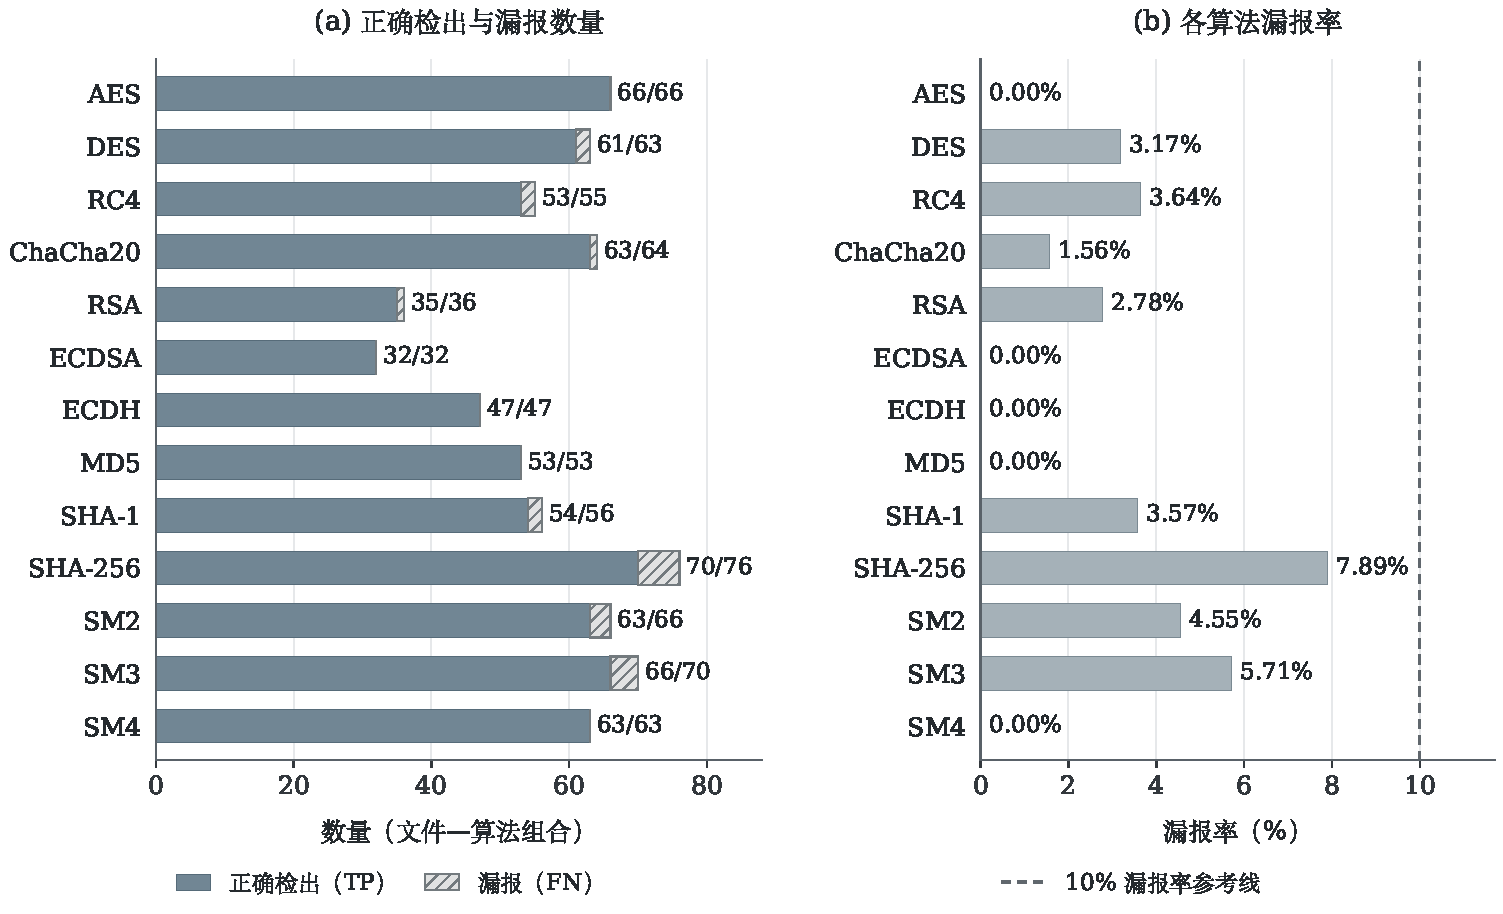
\includegraphics[width=\linewidth]{16-thirteen-algorithms.pdf}
\caption{十三种算法的正确检出、漏报数量及漏报率。左图标注为正确检出数/应检出数，斜线填充表示漏报；右图虚线表示 10\% 漏报率参考线。}
\label{fig:algorithm-suite-algorithms}
\end{figure}

\subsection{源码与二进制程序的识别结果}

表~\ref{tab:algorithm-suite-kinds} 列出源码与两种架构二进制程序的识别结果。154 份源码的召回率为 99.05\%，527 份 x86-64 二进制程序与 390 份 ARM64 二进制程序分别为 97.51\% 和 96.09\%。源码组漏报 1 项，二进制程序组共漏报 20 项。源码分析利用词法、定义及直接依赖信息，二进制程序分析则依据编译后可恢复的字节特征与运算关系。由于三组材料的实现来源和算法构成不同，不能仅据上述差异判断载体或架构对识别效果的影响。本组 1071 份文件不含固件镜像，固件采用独立的镜像集合评价提取与识别结果。

\begin{table}[H]\centering\small
\caption{源码与不同架构二进制程序的识别结果}
\label{tab:algorithm-suite-kinds}
\begin{tabularx}{\linewidth}{@{}Xrrlrr@{}}\toprule
检测对象 & 文件 & 应检出数 & TP/FP/FN & 召回率 & 漏报率\\\midrule
源码 & 154 & 105 & 104/0/1 & 99.05\% & 0.95\%\\
x86-64 二进制程序 & 527 & 361 & 352/0/9 & 97.51\% & 2.49\%\\
ARM64 二进制程序 & 390 & 281 & 270/0/11 & 96.09\% & 3.91\%\\\bottomrule
\end{tabularx}
\end{table}

% 配图依据：full-suite-rescan/scan/summary.json；由 plot_carriers.py 重算39个单元格并核对算法、载体两方向合计。
% 保留 ChaCha20 源码子组 1/8，不将标注边界通过重命名或删样本消除。
\begin{figure}[H]\centering
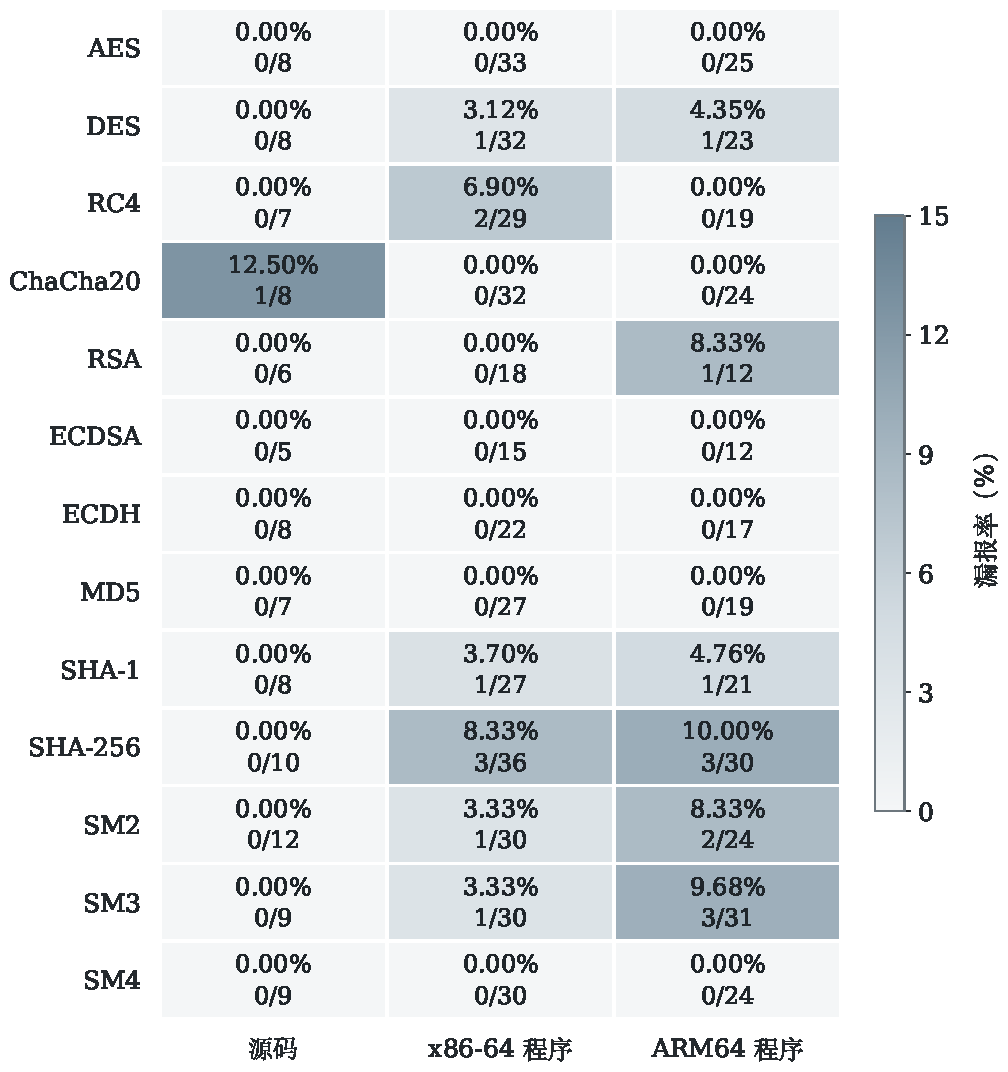
\includegraphics[width=.9\linewidth,height=.72\textheight,keepaspectratio]{17-thirteen-carriers.pdf}
\caption{十三种算法在源码、x86-64 和 ARM64 分组中的漏报分布。单元格上行为漏报率，下行为漏报数/应检出数。}
\label{fig:algorithm-suite-carriers}
\end{figure}

图~\ref{fig:algorithm-suite-carriers} 进一步展示算法与载体交叉分组的漏报情况。源码组中十二种算法均无漏报，ChaCha20 保留 1/8 的原正标签未检出。对该文件的复核发现，其循环实际执行八轮变换，属于 ChaCha8，与原 ChaCha20 标注不一致。为保持固定清单的评分口径，该项仍按原标签计入漏报，并单独说明变体差异。因此，算法总体漏报率低于 10\% 并不意味着所有载体子组都达到同一水平。

全部 1071 份文件均完成分析，未出现部分完成或失败。在 16 进程并发条件下，整批扫描耗时 498.03 秒。该耗时为单次运行记录，仅用于说明本组实验的处理成本。

\section{源码参考库消融实验结果}
\label{sec:expanded-source-results}

\subsection{参考补充对总体识别结果的影响}

表~\ref{tab:expanded-source-ablation} 给出 363 份源码、318 个实现正标签上的配对结果。两组固定检测器代码、输入及可见上下文，仅将源码参考库由 149 条扩充至 226 条。补充前正确检出 225 个正标签，漏报 93 个；补充后正确检出 306 个，漏报降至 12 个。召回率由 70.75\% 提高到 96.23\%，精确率由 99.56\% 变为 99.67\%。

\begin{table}[H]\centering\small
\caption{参考库补充前后的源码识别结果}
\label{tab:expanded-source-ablation}
\begin{tabularx}{\linewidth}{@{}Xrlrrr@{}}\toprule
参考库 & 记录数 & TP/FP/FN & 召回率 & 精确率 & 漏报率\\\midrule
原参考库 & 149 & 225/1/93 & 70.75\% & 99.56\% & 29.25\%\\
扩充参考库 & 226 & 306/1/12 & 96.23\% & 99.67\% & 3.77\%\\\bottomrule
\end{tabularx}
\end{table}

逐文件比较表明，补充参考记录增加了 81 个正确标签，未丢失原有正确检出，误报数量保持为 1，召回率提高 25.47 个百分点。新增 77 条记录中存在多算法模块，因此记录增量与标签增量并非一一对应。该配对结果反映固定代码条件下已知内容覆盖的变化，两组均保留其他识别通道。

两组均有 362 份源码正常完成、1 份部分完成，未出现失败。部分完成文件中的 ECDH 已被参考记录识别，但两个函数的结构分析达到节点预算上限，故其处理状态仍保留为部分完成。补充前后批次耗时分别为 70.72 秒和 72.14 秒；测量期间存在并发任务，仅据此记录处理规模，不将二者之差解释为参考库扩充的运行代价。

\subsection{来源分组结果与剩余误差}

表~\ref{tab:expanded-source-cohorts} 将参考补充及标签变化按材料来源分组。新增 77 条参考全部取自该源码集合，其中 59 条来自 110 份历史验证来源源码，占该子组文件数的 53.64\%。原参考库已有 120 条记录与待测源码内容重叠，扩充后增至 197 条。因此，该实验评价已观察材料上的版本覆盖，“历史验证来源”仅表示材料原始出处。

\begin{table}[H]\centering\small
\caption{不同来源源码的参考补充与识别结果}
\label{tab:expanded-source-cohorts}
\begin{tabularx}{\linewidth}{@{}Xrrrll@{}}\toprule
来源 & 文件 & 应检出数 & 新增参考 & 补充前 & 补充后\\\midrule
原固定源码 & 154 & 103 & 0 & 103/0/0 & 103/0/0\\
其他历史开发源码 & 71 & 72 & 1 & 70/0/2 & 71/0/1\\
历史验证来源源码 & 110 & 115 & 59 & 41/0/74 & 104/0/11\\
新审核模块 & 28 & 28 & 17 & 11/1/17 & 28/1/0\\
合计 & 363 & 318 & 77 & 225/1/93 & 306/1/12\\\bottomrule
\end{tabularx}
\par\smallskip\raggedright\footnotesize 注：补充前、补充后两列均按 TP/FP/FN 表示。
\end{table}

历史验证来源子组增加 63 个正确标签，召回率由 35.65\% 提高到 90.43\%，误报仍为零，是总体增益的主要来源。由于其中 59 份源码已参与参考库构建，该结果表明相应版本纳入参考后的覆盖改善，不再具有独立测试的含义。新审核模块增加 17 个正确标签，其他历史开发源码增加 1 个，原固定源码的预测保持不变。

本组对原固定源码采用经核查的 103 个正标签：一份 ChaCha8 和一份仅含四分之一轮的源码均保留为输入，但不赋予完整 ChaCha20 标签。该组的 103/0/0 与上一节的 104/0/1 因评分范围不同而形成，实际预测一致，不属于新增检出。

表~\ref{tab:expanded-source-algorithms} 列出扩充参考库后的逐算法结果。各算法包含 20--55 个正标签，漏报率均不超过 10\%。DES、RC4、ECDSA、ECDH 和 MD5 无漏报；SHA-1 的漏报率最高，为 9.09\%。ECDH 同时出现 1 项误报，说明正标签覆盖与算法身份判定仍需分别考察。

\begin{table}[H]\centering\small
\caption{扩充参考库后的逐算法源码识别结果}
\label{tab:expanded-source-algorithms}
\begin{tabularx}{\linewidth}{@{}Xrlrr@{}}\toprule
算法 & 应检出数 & TP/FP/FN & 召回率 & 漏报率\\\midrule
AES & 55 & 53/0/2 & 96.36\% & 3.64\%\\
DES & 20 & 20/0/0 & 100.00\% & 0.00\%\\
RC4 & 20 & 20/0/0 & 100.00\% & 0.00\%\\
ChaCha20 & 20 & 19/0/1 & 95.00\% & 5.00\%\\
RSA & 26 & 24/0/2 & 92.31\% & 7.69\%\\
ECDSA & 21 & 21/0/0 & 100.00\% & 0.00\%\\
ECDH & 21 & 21/1/0 & 100.00\% & 0.00\%\\
MD5 & 21 & 21/0/0 & 100.00\% & 0.00\%\\
SHA-1 & 22 & 20/0/2 & 90.91\% & 9.09\%\\
SHA-256 & 31 & 29/0/2 & 93.55\% & 6.45\%\\
SM2 & 21 & 20/0/1 & 95.24\% & 4.76\%\\
SM3 & 20 & 19/0/1 & 95.00\% & 5.00\%\\
SM4 & 20 & 19/0/1 & 95.00\% & 5.00\%\\\bottomrule
\end{tabularx}
\end{table}

12 个漏报中有 11 个位于历史验证来源子组，另一个位于其他历史开发源码。漏报文件涉及实现主体委托、可见上下文不足和硬件专用表示等情况。唯一误报位于 LibreSSL 的 SM2 加解密模块，共享椭圆曲线点运算额外触发 ECDH 标签，反映出公共数学结构与具体协议用途之间的区分仍不充分。

\section{固件镜像识别结果}
\label{sec:firmware-results}

\subsection{镜像提取与终端覆盖}

本组以五类终端的 10 份自制 SquashFS 镜像为检测对象，每类分别提供 x86-64 和 ARM64 版本。扫描器直接接收原始镜像，提取内部文件后执行静态分析，镜像内部不包含源码。全部镜像均完成提取与扫描，共恢复 650 个文件，其中二进制文件 540 个。恢复文件的路径和内容摘要与独立交付清单逐项一致，未发现组件遗漏或内容变化。

每份镜像含 65 个文件，其中 54 个为二进制文件。除原业务程序及其密码库外，另有十三种算法的 13 个共享库和 39 个静态链接程序。三个程序变体分别处理原始输入、带长度字段的记录及带终端任务标识的记录，所需算法代码均实际链接于文件内部。十份镜像共有 530 个文件包含密码实现，其他文件仅保留运行所需配置、输入、说明和许可。共享库保留导出接口，离线程序保留普通符号表，故本组包含不同符号条件，不能统一解释为去符号识别成绩。

五类 x86-64 镜像中的 65 个新增共享库、195 个新增程序均通过功能检查，5 个原业务程序也通过预期输出核对。九种对称或摘要算法的已知答案检查通过，RSA、ECDSA 和 SM2 完成正常签名验签与篡改拒绝检查，ECDH 双方所得共享秘密一致。新增程序可独立处理本地输入，但未自动接入原业务服务，不将组件存在等同于业务已启用全部算法。ARM64 仅完成构建、提取与静态扫描。

\begin{table}[H]\centering\small
\caption{五类终端固件的提取与实现识别结果}
\label{tab:terminal-coverage-results}
\begin{tabularx}{\linewidth}{@{}Xrrrl@{}}\toprule
终端软件类型 & 镜像 & 提取文件 & 二进制文件 & TP/FP/FN\\\midrule
智能电能表 & 2 & 130 & 108 & 131/0/9\\
用电信息采集集中器 & 2 & 130 & 108 & 131/0/9\\
配电自动化终端（FTU） & 2 & 130 & 108 & 131/0/9\\
继电保护装置（IED） & 2 & 130 & 108 & 131/1/9\\
电力边缘网关 & 2 & 130 & 108 & 133/0/9\\
合计 & 10 & 650 & 540 & 657/1/45\\\bottomrule
\end{tabularx}
\end{table}

\subsection{算法识别与误差分析}

算法评价以组件的“文件--算法”组合为单位，对清单声明的全部 540 个二进制文件，在十三种目标算法范围内评分。RSA、ECDSA 和 ECDH 组件中的 SHA-256，以及 SM2 组件中的 SM3，均按实际链接内容计入真值。同一算法在多个文件中出现分别计数，同一文件的重复证据合并。文本、配置及许可文件不参与实现评分，本组结果也不与前述 1071 份文件合并计算。

共计 702 项应检出的算法实现，正确检出 657 项，误报 1 项，漏报 45 项。总体召回率为 93.59\%，精确率为 99.85\%，漏报率为 6.41\%。表~\ref{tab:firmware-algorithm-results} 给出逐算法结果，十三种算法均在本组获得正确检出，但不同算法及架构的覆盖并不相同。

\begin{table}[H]\centering\small
\caption{固件镜像内部组件的算法识别结果}
\label{tab:firmware-algorithm-results}
\begin{tabularx}{\linewidth}{@{}Xrlrr@{}}\toprule
算法 & 应检出数 & TP/FP/FN & 召回率 & 精确率\\\midrule
AES & 44 & 44/0/0 & 100.00\% & 100.00\%\\
DES & 40 & 40/0/0 & 100.00\% & 100.00\%\\
SM4 & 44 & 24/0/20 & 54.55\% & 100.00\%\\
RC4 & 40 & 15/0/25 & 37.50\% & 100.00\%\\
ChaCha20 & 40 & 40/0/0 & 100.00\% & 100.00\%\\
MD5 & 42 & 42/0/0 & 100.00\% & 100.00\%\\
SHA-1 & 42 & 42/1/0 & 100.00\% & 97.67\%\\
SHA-256 & 170 & 170/0/0 & 100.00\% & 100.00\%\\
SM3 & 80 & 80/0/0 & 100.00\% & 100.00\%\\
RSA & 40 & 40/0/0 & 100.00\% & 100.00\%\\
ECDSA & 40 & 40/0/0 & 100.00\% & 100.00\%\\
ECDH & 40 & 40/0/0 & 100.00\% & 100.00\%\\
SM2 & 40 & 40/0/0 & 100.00\% & 100.00\%\\
合计 & 702 & 657/1/45 & 93.59\% & 99.85\%\\\bottomrule
\end{tabularx}
\end{table}

按架构汇总，x86-64 组件的 TP/FP/FN 为 346/1/5，ARM64 为 311/0/40。漏报集中于新增 RC4 和 ARM64 SM4 组件：五份 x86-64 RC4 共享库未确认实现，每份 ARM64 镜像中新增的 RC4 共享库及三个程序、SM4 共享库及三个程序均未确认。相关代码已经通过原生功能检查或构建清单审核，缺少识别标签反映当前检测覆盖不足，不能据此否定文件中存在相应实现。唯一误报仍位于 x86-64 继电保护装置的原密码库，实际包含 MD5 和 SHA-256，却额外报告 SHA-1。

算法证据可通过镜像摘要、内部路径及组件摘要回到交付文件。上述结果验证了较多密码组件共存时的提取、识别与定位流程，但多个终端、程序变体及架构复用上游实现，新增文件数量不代表独立实现来源的增加。镜像也不包含完整设备启动环境，因此不能据此推断真实厂商固件或未收录实现的识别水平。

\section{前端应用实验结果}
\label{sec:frontend-results}

本节选取上述电力边缘网关的 x86-64 镜像，验证工作台从任务创建到报告导出的应用流程。该样例复用固件实验中的输入，页面任务单独执行，其识别结果不作为新增独立样本重复计数。

\subsection{网关检测结果与证据定位}

网关镜像大小为 4132864 字节，包含 54 个二进制文件及必要配置、输入与许可材料。工作台独立创建任务后恢复 65 个文件，所有组件均正常完成。服务端端到端耗时为 136.54 秒，包含交付核验、解包、扫描与结果写出，不含浏览器传输和人工查看时间。该数值为本次应用验证的单轮记录。

结果形成 70 条已识别资产记录，涉及全部十三种算法，其中 16 条标为“量子迁移关注”，15 条标为“遗留算法关注”。资产按组件、算法及证据类别归并，多条命中不重复增加记录。一份组件可含多个算法，因此资产记录数与二进制文件数分别统计。图~\ref{fig:gateway-workbench-results} 以维护任务名称及量子迁移关注为筛选条件，展示 RSA、ECDSA、ECDH 和 SM2 的四条记录，均可进入对应组件的证据详情。

% 实际网关任务截图；筛选仅控制页面显示，不修改完整扫描或评分结果。
\begin{figure}[H]\centering
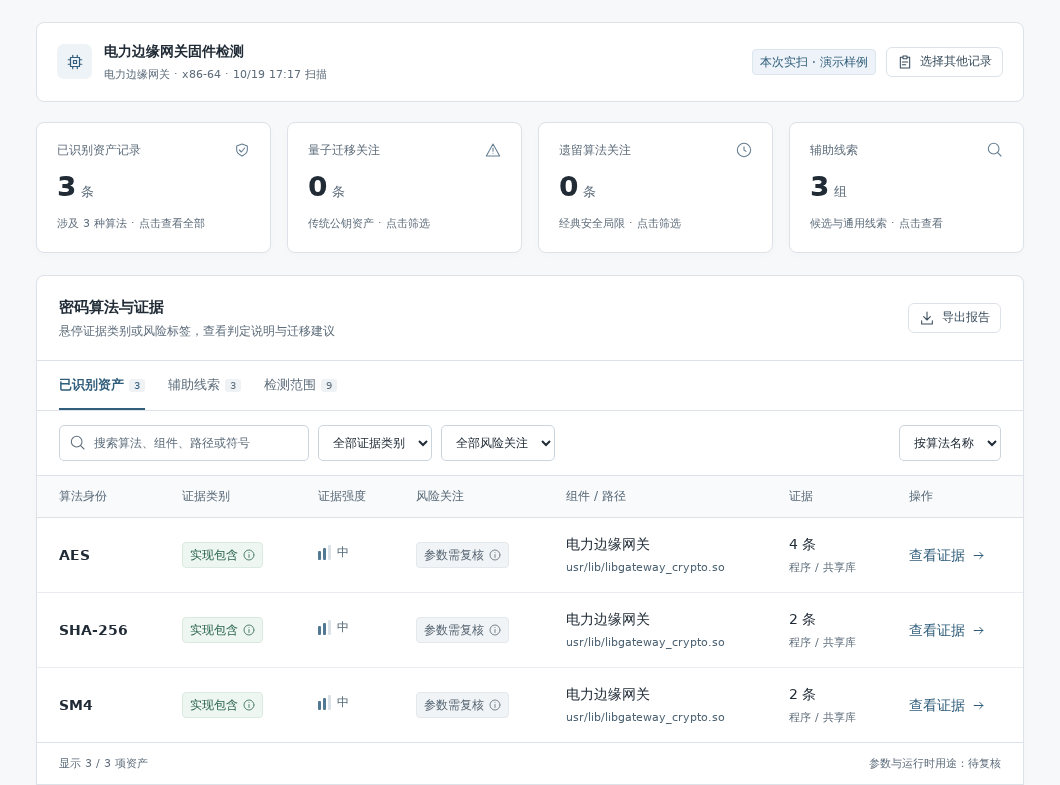
\includegraphics[width=\linewidth]{20-gateway-workbench-results.png}
\caption{网关的资产汇总及量子迁移关注筛选结果，列表展示部分公钥算法组件。}
\label{fig:gateway-workbench-results}
\end{figure}

结果另有 49 组辅助线索，单独保留候选名称与原始依据，不计入已识别资产。“量子迁移关注”用于提示传统公钥机制的替换评估，“遗留算法关注”用于提示 DES、RC4、MD5 和 SHA-1 的经典安全局限，其他资产仍需核对参数及用途。新增程序中的固定密钥只用于实验，不作为部署配置建议。静态结果没有证明全部算法均被原网关业务实际使用。

组件树包含外层镜像及 65 个提取文件，共 66 个条目。图~\ref{fig:gateway-workbench-components} 展示其中的镜像和密码组件，支持由算法回到文件位置。镜像摘要、内部路径和组件摘要在交付清单、独立提取结果及扫描报告中一致。该层级来自包含与提取关系，不表示组件调用或业务依赖。

\begin{figure}[H]\centering
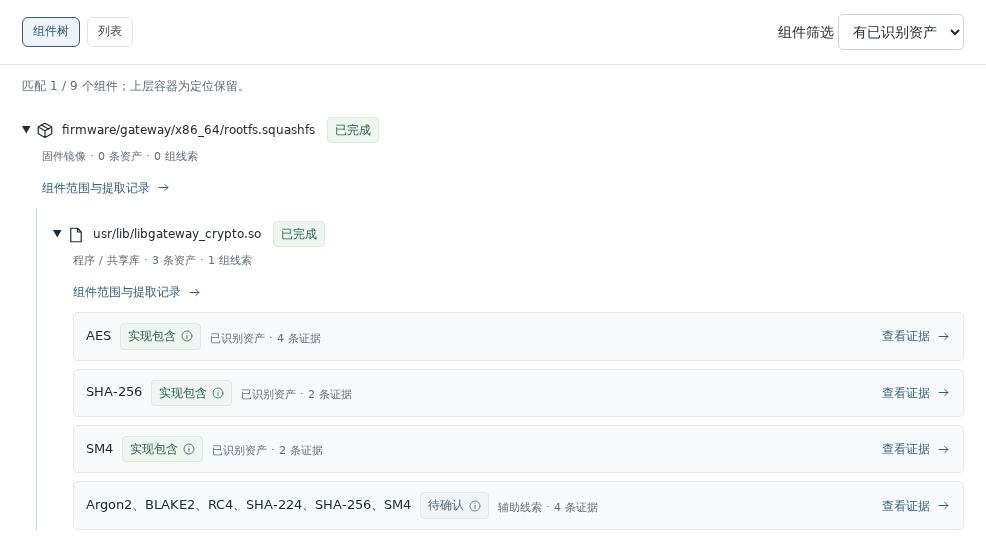
\includegraphics[width=\linewidth]{21-gateway-workbench-components.png}
\caption{网关镜像与内部密码组件的定位关系，视图展示组件树的一部分。}
\label{fig:gateway-workbench-components}
\end{figure}

以原密码库中的 AES 为例，证据详情同时列出数据表和参考函数匹配依据，记录参考函数 \texttt{aes\_encrypt}、文件偏移 \texttt{0x34e0}、匹配长度及引用数据约束。图~\ref{fig:gateway-workbench-evidence} 展示该条参考匹配。新增签名和密钥协商组件则可查看相应函数定义证据及文件位置，按其实际证据类别复核，不将符号定义识别解释为去符号算法恢复。

% 参考函数记录对应静态文件内容，不代表运行时调用或完整算法等价证明。
\begin{figure}[H]\centering
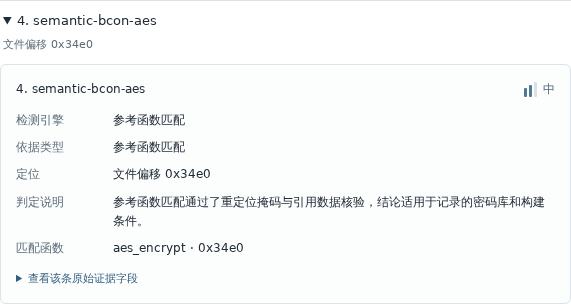
\includegraphics[width=.88\linewidth]{22-gateway-workbench-evidence.png}
\caption{AES 参考函数匹配的证据详情，包含函数名称、文件偏移和原始字段入口。}
\label{fig:gateway-workbench-evidence}
\end{figure}

\subsection{报告一致性与界面验证结果}

汇总 JSON、原始证据 JSON、CSV 表格和 Markdown 文本报告均保留 70 条已识别资产及 49 组辅助线索，任务标识与原始扫描一致。原始证据报告同时包含镜像与组件记录，可在页面之外核对输入身份及证据位置。搜索或风险筛选仅影响当前列表，导出文件仍保留完整任务结果。图~\ref{fig:gateway-workbench-report} 为同一任务的中文报告预览。

\begin{figure}[H]\centering
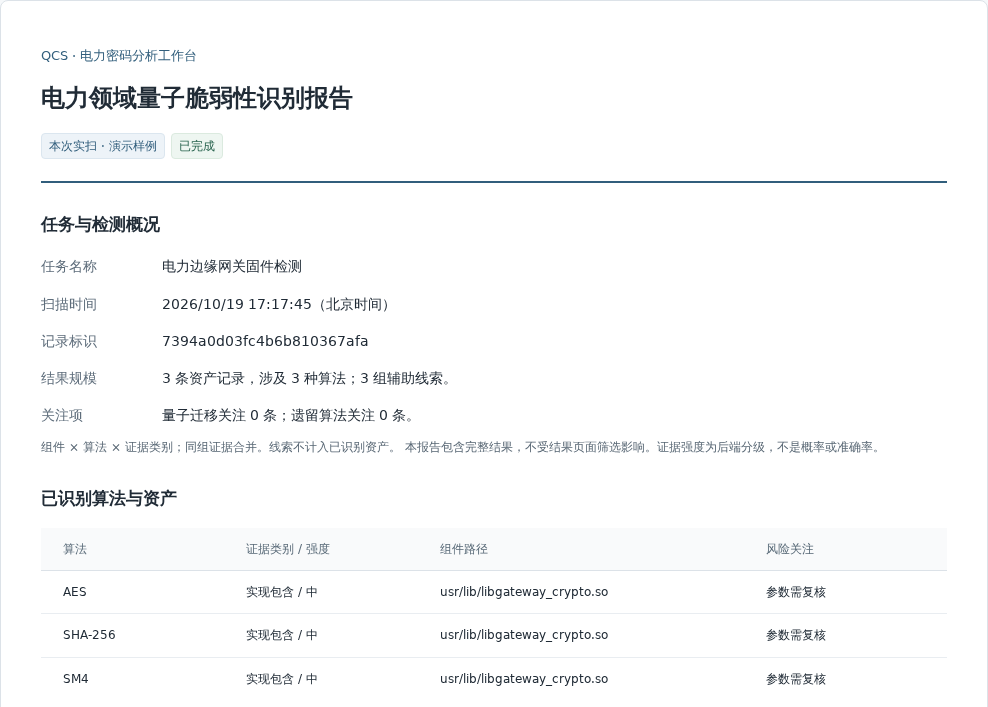
\includegraphics[width=\linewidth]{23-gateway-workbench-report.png}
\caption{网关任务的中文报告预览，汇总数值与页面及下载文件一致。}
\label{fig:gateway-workbench-report}
\end{figure}

中文报告经浏览器打印生成 32 页 A4 文档，包含资产清单、证据摘要、辅助线索与检测边界。Chromium 145 中的任务创建、结果检索、风险筛选、证据展开、组件定位及四种格式下载均正常完成，刷新后仍可读取任务结果。无匹配搜索显示空结果提示，在 1280 和 1440 像素宽度下均未出现整体横向溢出，交互过程中未发现未捕获的脚本异常。另从上传入口提交同版本镜像，核对接收摘要、组件数和算法种类，以确认新增镜像能够用于用户上传演示。

\section{结果讨论与适用范围}

已知实现集合的 97.19\% 召回率与源码参考补充后的 96.23\% 召回率分别对应不同材料和评分范围，不能合并为总体性能。前者的样本参与过规则与参考库修订，后者新增参考全部取自被测集合，均主要反映已知版本覆盖。作为对照背景，早期检测版本在 2855 份历史输入上的 TP/FP/FN 为 684/6/771，召回率为 47.01\%，显示不同实现与构建条件下仍存在明显缺口。由于材料、版本和评分范围不一致，该历史成绩仅用于说明外部有效性的限制，不与主体实验计算提升幅度。

受限语义后端在 18 组指令片段检查和 208 组数值对照中通过局部核查，但三批共 3339 份历史输入在接入前后的文件级算法预测没有变化，直接新增标签为零。因而，位宽及输入依赖约束具有局部结构检查依据，其对整体召回率的贡献尚未获得该对照支持。参考匹配、运算分析及语义后端的作用需要通过各自的消融结果评价，不能由综合成绩反推某一通道的独立增益。

错例同时反映出算法身份与分析完成度的区别。共享数学操作可能触发错误的协议标签，缺少实现主体或必要上下文则可能导致漏报；参考标签被识别后，受预算限制的结构分析仍可能部分完成。算法名称、证据位置、参数和处理状态应分别解释，才能避免以单个标签替代对完整实现及其用途的判断。

五类终端和网关均采用自制文件系统镜像，密码实现来源明确，部分与参考库共享来源，结果支持受控软件范围内的提取、识别和复核流程。真实厂商交付物、实体设备运行及后量子协议替换未在该应用实验中验证。界面风险提示用于引导参数与用途核查，尚不能作为网关整体抗量子安全结论。GraphRAG 和本地大模型仍处于方案设计阶段，本章不对其关联分析效果或运行开销作实测结论。

\section{本章小结}

已知实现覆盖实验在 1071 份输入、747 个正标签上取得 726/0/21 的 TP/FP/FN，召回率为 97.19\%。源码参考库消融在固定代码和材料条件下，将召回率由 70.75\% 提高到 96.23\%，增加 81 个正确标签，误报数量不变。分组与错例分析表明，已审核参考记录能够改善相应版本的覆盖，共享结构、上下文缺失及标注边界仍影响具体判断。

固件镜像实验完成五类终端共 10 份镜像的提取，恢复 650 个文件，其中 540 个二进制文件的 TP/FP/FN 为 657/1/45，召回率为 93.59\%，精确率为 99.85\%。网关前端应用实验形成 70 条资产记录，涉及十三种算法，并保持组件来源、证据位置及导出报告的一致性。上述结果支持受控软件材料的密码资产核查，未知实现覆盖与真实业务部署仍需进一步评价。

\chapter{总结与展望}\section{工作总结}
本文完成了基于已实现 QCS 工程的原理、方案、结果与应用整理。
检测引擎通过源码、符号、字节、已知函数和运算语义通道，
将源码、程序及受支持固件组织为可追溯证据；
国密模块扩充 SM2、SM3、SM4，可选 Miasm 提供有限 CFG、保守合并及带输入身份的摘要。
报告区分接口引用、实现包含与运行时使用，
保留未知配置、共享结构、预算耗尽与失败状态。

本轮将算法主实验扩展至理论章节的全部十三种核心算法，
从开发总体全取源码与 x86-64/ARM64 程序，共 1071 份不同内容输入实际新扫，
TP/FP/FN 为 700/0/47，总体实现召回率 93.71\%、漏报率 6.29\%。
逐算法的漏报目标为不超过 10\%，表格保留绝对数、达标状态和分载体差异。
该结果是已知家族回归，原五算法筛选混合演示、
完整开发、历史覆盖和 Miasm 收益对照继续保留，支持进一步复核。
作品优势仍是证据可审查、多载体接入与资源可控，
未来需要用新的独立实现验证更广范围的覆盖。

GridLens 把识别结果落到虚拟电力边缘网关的发布前体检：
四组件、两版本、两架构和六文件范围形成可演示闭环，
遗留摘要变化有真实源码及扫描证据，公钥迁移保持人工待办。
离线网页与本地服务使演示不依赖实体硬件；这一可用性成果与泛化指标分别评价。
另补齐五类电力终端的软件级场景：不同业务程序与独立清单构成 10 份双架构自制固件，
实际解包核验 80 个文件并扫描 20 个 ELF；22 个正标签全部检出，保留一项误报。
五类 x86-64 业务检查通过，ARM64 只完成静态验证；
这些证据支持固件软件流程，不等同于真实厂商或实体终端覆盖。

\section{后续改进路线}
\subsection{优先提升未知实现覆盖}
首先针对大数与曲线算法建立带 ABI、参数身份、输出缓冲区、成功路径和调用副作用的摘要。
由模乘、Montgomery 约减、模逆、模幂和点运算关系逐步组合成算法见证，
避免仅凭乘法或点乘命名协议。
对 SHA-256、SM3、SM4 继续扩大开发实现多样性，
验证轮常量使用、动态查表、位切片、硬件指令和优化下的数据依赖。
新规则必须先在开发范围完成正反例与预算检验。

\subsection{完善语义与资源边界}
继续处理 Thumb IT、MIPS 延迟槽、调用摘要及别名内存输出，
改进候选选择和启动成本，并检查预算不足时的稳定弃权。
原语或部分表达式不能被包装成整个函数恢复，
也不把生成伪代码后再做名称扫描作为覆盖提升的充分证据。
既有 ARM 探针异常和预算相关回归需要单独修复，再运行相应验证。

\subsection{提高评测的外部有效性}
重新冻结后保留未见作者与构建链的独立留出集合，
按家族汇总并报告各算法、架构、载体和不完整状态。
完整开发、历史观察与演示筛选继续分离，
不在看到留出结果后挑选最有利变体再称其为独立性能。
如需比较其他工具或模型，应固定同一真值、输出范围、预算和计数单位，
不能用各自论文的数字拼接排行榜。

\subsection{从迁移辅助走向工程验证}
在应用层补充配置证据、证书链、依赖版本与标准 CBOM 导出，
再验证真正的网关进程、升级签名、防回滚、消息认证和密钥生命周期。
后量子或混合协议应经过测试向量、互操作、资源开销及接收端兼容实验，
完成这些证据后才能把候选路线改为已验证迁移结果。
Windows 原生与 WSL 的安装演示、真实设备或受控模拟环境也应单独验收。

\section{结语}
发布前密码资产体检的首要价值，是把不可见的密码依赖变成可定位、可解释、
可复查的对象，并为迁移决策保留明确证据。
本作品已经实现这一软件原型及应用展示；未知实现识别与端到端迁移验证仍是下一阶段的核心工作。

\backmatter\renewcommand{\bibname}{参考文献}
\bibliographystyle{plain}\bibliography{bib/references}
\end{document}
